\documentclass[11pt]{report}
\usepackage[utf8]{inputenc}

\usepackage{floatrow}
\usepackage{graphicx}
\usepackage{caption}
\usepackage[parfill]{parskip}
\usepackage[backend=bibtex]{biblatex}
\usepackage{pgfplots}
\usepackage{xcolor}
\usepackage{fixltx2e}


\usepackage{listings}
\usepackage{color}

\usepackage[autostyle]{csquotes}

%\usepackage[none]{hyphenat} %Choose one
\tolerance=1
\emergencystretch=\maxdimen
\hyphenpenalty=10000
\hbadness=10000


%START JSON DEF
\colorlet{punct}{red!60!black}
\definecolor{background}{HTML}{EEEEEE}
\definecolor{delim}{RGB}{20,105,176}
\colorlet{numb}{magenta!60!black}


\definecolor{bblue}{HTML}{4F81BD}
\definecolor{rred}{HTML}{C0504D}
\definecolor{ggreen}{HTML}{9BBB59}

\lstdefinelanguage{json}{
    basicstyle=\normalfont\ttfamily,
    numbers=left,
    numberstyle=\scriptsize,
    stepnumber=1,
    numbersep=8pt,
    showstringspaces=false,
    breaklines=true,
    frame=lines,
    backgroundcolor=\color{background},
    literate=
     *{0}{{{\color{numb}0}}}{1}
      {1}{{{\color{numb}1}}}{1}
      {2}{{{\color{numb}2}}}{1}
      {3}{{{\color{numb}3}}}{1}
      {4}{{{\color{numb}4}}}{1}
      {5}{{{\color{numb}5}}}{1}
      {6}{{{\color{numb}6}}}{1}
      {7}{{{\color{numb}7}}}{1}
      {8}{{{\color{numb}8}}}{1}
      {9}{{{\color{numb}9}}}{1}
      {:}{{{\color{punct}{:}}}}{1}
      {,}{{{\color{punct}{,}}}}{1}
      {\{}{{{\color{delim}{\{}}}}{1}
      {\}}{{{\color{delim}{\}}}}}{1}
      {[}{{{\color{delim}{[}}}}{1}
      {]}{{{\color{delim}{]}}}}{1},
}
%END JSON DEF

%START BATCH DEF
\lstdefinelanguage{batch}{
    basicstyle=\normalfont\ttfamily,
    numbers=left,
    numberstyle=\scriptsize,
    stepnumber=1,
    numbersep=8pt,
    showstringspaces=false,
    breaklines=true,
    frame=lines,
    backgroundcolor=\color{background},
}
%END BATCH DEF


\def\signed #1{{\leavevmode\unskip\nobreak\hfil\penalty50\hskip2em
  \hbox{}\nobreak\hfil(#1)%
  \parfillskip=0pt \finalhyphendemerits=0 \endgraf}}

\newsavebox\mybox
\newenvironment{aquote}[1]
  {\savebox\mybox{#1}\begin{quote}}
  {\signed{\usebox\mybox}\end{quote}}

\newenvironment{nscenter}
 {\parskip=0pt\par\nopagebreak\centering}
 {\par\noindent\ignorespacesafterend}

\definecolor{dkgreen}{rgb}{0,0.6,0}
\definecolor{gray}{rgb}{0.5,0.5,0.5}
\definecolor{mauve}{rgb}{0.58,0,0.82}
\definecolor{highlight}{RGB}{255, 255, 0}

\lstset{frame=tb,
  language=Java,
  aboveskip=3mm,
  belowskip=3mm,
  showstringspaces=false,
  columns=flexible,
  basicstyle={\small\ttfamily},
  numbers=left,
  numberstyle=\tiny\color{gray},
  keywordstyle=\color{blue},
  commentstyle=\color{dkgreen},
  stringstyle=\color{mauve},
  breaklines=true,
  breakatwhitespace=true,
  tabsize=4,
  xleftmargin=2em,
  framexleftmargin=1.5em,
  postbreak=\raisebox{0ex}[0ex][0ex]{\ensuremath{\color{red}\hookrightarrow\space}}
}

\lstset{breaklines=true}

\newcommand*{\thead}[1]{\multicolumn{1}{| c |}{\bfseries #1}}

\addbibresource{references/references.bib}


\title{Master}
\author{Henrik M. Sivertsgård}

\begin{document}

  \begin{titlepage}
    \begin{center}
      \line(1,0){350}
      \\[1cm]
      \textsc{\LARGE Mobile data security and cloud storage}
      \\[1cm]
      \line(1,0){350}
    \end{center}
    Henrik Sivertsgård, HIB: H139734 : UIB: 212779 , henriksive@gmail.com
    \\[0.2cm]
    Supervisors: Marcus Bezem, Federico Mancini
    \\[0.2cm]
    \today
  \end{titlepage}
% !TEX root = ../Article.tex
\begin{abstract}

\end{abstract}

  \newpage
  \tableofcontents

  \listoffigures

  \listoftables

  \lstlistoflistings




  % !TEX root = ../Article.tex
\chapter{Introduction}
\section{Problem statement and motivation}
In todays society the standard commercial smartphone is considered secure by the average user. This statement is partially true as the regular user rarely encounters sensitive data apart from personal passwords. As the development on smartphones have skyrocketed new parties have expressed interest in smartphone capabilities. In relation to this there is now a need for the smartphone to handle sensitive data, e.g, health data, military intelligence and governmental information.

Handling senstive data in context of smartphones involves storing the data, processing the data and potentially sharing the data. In these areas there exists obstacles that needs to be dealt with in order to handle the sensitive data securely. Two of the biggest obstacles are being able to encrypt and decrypt data effectively and key management/storage.

 In a perfect world the smart phone would be able to overcome these obstacles by itself. Many mobile devices lack the capability to store keys securely and run operations in a secure environment and thus cannot execute all steps needed. A smart card cans provide a solution to these problems, but we have to investigate if the smart cards introduces new attack vectors and constraints.

\section{Goals}
\label{sec:goals}
The overall goal of this thesis is to explore and evaluate the possibilities of how smart cards and mobile devices can co-operate to achieve a higher level of information security. To better understand what limitations there are, we will need to create a framework for easy communication between a mobile device and smart card. This includes developing test applications for both the mobile device and the smart card. A framework, mobile application and smart card application allows us to test performance and security, with as close to real life use cases as possible.

In order to achieve this goal we will attempt to answer the following research questions:
\begin{itemize}
  \item ``What are the limitiations of smart cards in the context of hardware?''
  \item ``What are the limitiations of smart cards in the context of software?''
  \item ``What are the types of use cases we are able to solve and strengthen the security of using smart cards?''
\end{itemize}

%To achieve the overall goal we will need to look into a set of sub-goals. The sub-goals are as follows:
%\begin{enumerate}
%    \item Determine limitations on the smart card.
%    \item Identify use cases we are able to solve using smart cards.
%    \item Outline standards for solving use cases using smart cards.
%    \item Test the use cases with real-life data.
%\end{enumerate}

\section{Related work}
The Secure Element Evaluation Kit (SEEK) for the Android platform is an open source project, maintained by Giesecke \& Devrient GmbH \cite{Giesecke}, which have a vision to make it easier to use secure elements in Android applications. The framework provides access to a variety of secure elements such as SIM cards, micro SD cards and embedded secure elements. Their final goal is to have their library as an integrated part of the Android operating system such that all new mobile devices comes with hardware-backed security support \cite{SEEK}. However, their focus are on the Android platform, while this thesis will focus more on the smart card itself and what a smart card brings to the table security wise.

\section{Chapter introduction}
\paragraph{Chapter 1 - Introduction}
Presents a problem statement, motivation and research question for this master thesis.

\paragraph{Chapter 2 - Background}
Introduces all concepts needed for understanding how smart cards and relevant technology function. Gives a basic understanding for which threats exists for the platform.

\paragraph{Chapter 3 - Smart card framework}
Discusses the basis for the smart card communication framework, what goals we have for the framework and describes how we are going to work when developing the framework.

\paragraph{Chapter 4 - Challenges}
Identifies and examines challenges that have emerged when trying to use smart cards in co-operation with mobile devices. Presents and evaluates a solution for the problems.

\paragraph{Chapter 5 - Framework Implementation}
Gives an overview of how the framework is implemented and structured using code examples and diagrams.

\paragraph{Chapter 6 - Test cases}
Shows the testing environment for the smart cards and provides detailed testing results for smart card limitations and use cases.

\paragraph{Chapter 7 - Discussion and Conclusion}
Discusses the research questions that we have established and what experiences we encountered during this master thesis.

  % !TEX root = ../Article.tex
\chapter{Background}
In this chapter we will provide background information necessary to understand how smart cards function and can increase security on mobile devices. The topics covered in this section are smart cards, mobile device operating systems, cryptography and threats in context of mobile devices.

\section{Smart Card}
\label{sec:smartcard}
A smart card refers to a credit card sized card with an integrated circuit, usually in the form of a plastic card with an integrated micro processor. In essence a smart card is a miniature computer with limited computing power.

\subsection{Smart card architecture}
The micro processor is able to perform tasks that involve processing input, give ouput and storing small amounts of data. Smart cards vary in sizes defined by the standards ISO/IEC 7810 \cite{iso7810} and ISO/IEC 7816 \cite{iso7816}. The processing power of smart cards are between 25-32 MHz and sport anywhere from 8Kbit to 128Kbit memory (EEPROM) \cite{cardProcessing}.

The micro processor can be powered and communicate in two ways. Contact smart cards have integrated contact pads. When the smart card is inserted into a card reader the contact pads of the card reader provides power to the micro processor via the contact pads of the smart card. The contact pads also functions as a medium for transferring data. Contactless smart cards uses radio-frequency induction to power the micro processor and to transmit data between an antenna and the card. Most modern smart cards supports both technologies (hybrid cards). Figure \ref{fig:nfccard} is a blank hybrid card.

An everyday example of a smart card is the modern credit and debit card. Most of these cards are contact cards that require the user to insert the card into a card reader, but newer cards are of the hybrid type, and have the ability to communicate over radio frequencies. Credit and debit cards utilizes the input/output capabilities of the smart card, but they also store information on the card authenticating the users bank information.

\begin{figure}[h!]
  \caption{Hybrid Smart card.}
  \label{fig:nfccard}
  \centering
    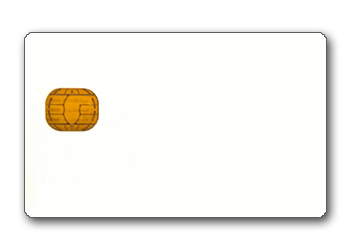
\includegraphics[width=0.75\textwidth]{images/nfccard2.png}
\end{figure}

\subsection{Communication standard for smart cards}
\label{sec:communicationstandard}
Application Protocol Data Unit (APDU) is a standard that describes how a smart card application should communicate with other applications (off-card) and is defined by ISO7816-4 \cite{iso7816-4}. There are two types of APDU messages: Command APDU and Response APDU.

Command APDU is split into header and body. Refer to table \ref{tbl:cmdAPDU} for instruction explanation and summary. The header is mandatory for all transactions and consists of 4 bytes that is split into CLA, INS, P1 and P2. The body of a command APDU is split into 3 parts; LC, Payload and LE. LC is 1 byte, payload is maximum 255 bytes and LE is 1 byte.

Newer smart cards supports Extended APDU which allows the payload to be up to a maximum of 65535 bytes. If the payload data is greater than 255 bytes LC must be 3 bytes where the first byte is 0x00 to denote that the APDU is extended and the remaining 2 bytes denotes the length. If extended APDU is used then LE consists of 2 bytes to account for longer responses.
\begin{table}[h!]
\caption{Command APDU layout.}
\label{tbl:cmdAPDU}
\centering

    \begin{tabular}{ | l | c | l |}
        \hline
        \thead{Name}
        & \thead{Number of bytes}
        & \thead{Description} \\ \hline

        CLA  & 1 & Command type class, type of command \\ \hline
        INS & 1 & Instruction code, command to run \\ \hline
        P1 & 1 & Free parameter \\ \hline
        P2 & 1 & Free parameter \\ \hline
        LC & 0, 1 or 3 & Length of payload \\ \hline
        Payload & 0 - 65535 & Payload data \\ \hline
        LE & 0, 1 or 2 & Expected response length \\ \hline

    \end{tabular}

\end{table}


Response APDU is split into body and response trailer. The body consist of the response data and is at maximum 255 bytes or 65535 bytes depending on if extended APDU is used. All response APDUs must contain a response trailer of two bytes which denotes the processing status (error, success, wrong format, etc.) of the command APDU. Refer to table \ref{tbl:rspAPDU} for definitions and summary.
\begin{table}[h!]
\caption{Response APDU layout.}
\label{tbl:rspAPDU}
\centering

    \begin{tabular}{ | l | c | l |}
        \hline
        \thead{Name}
        & \thead{Number of bytes}
        & \thead{Description} \\ \hline

        Response & 0-65535 & Response data \\ \hline
        SW1+SW2 & 2 & Command processing status \\ \hline

    \end{tabular}

\end{table}


To better understand when to use the command APDUs and when to use response APDUs can use the following example: A locked door has a card reader connected to it. A person walks up to the door and presents his contactless smart card to the reader. The card reader sends a command APDU to the card asking for the ID. The smart card processes the command APDU and sends a response APDU back to the card reader containing the ID of the person. This example is visualized in figure \ref{fig:doornfc}.

\begin{figure}[h!]
  \caption{Door lock using smart card to unlock.}
  \label{fig:doornfc}
  \centering
    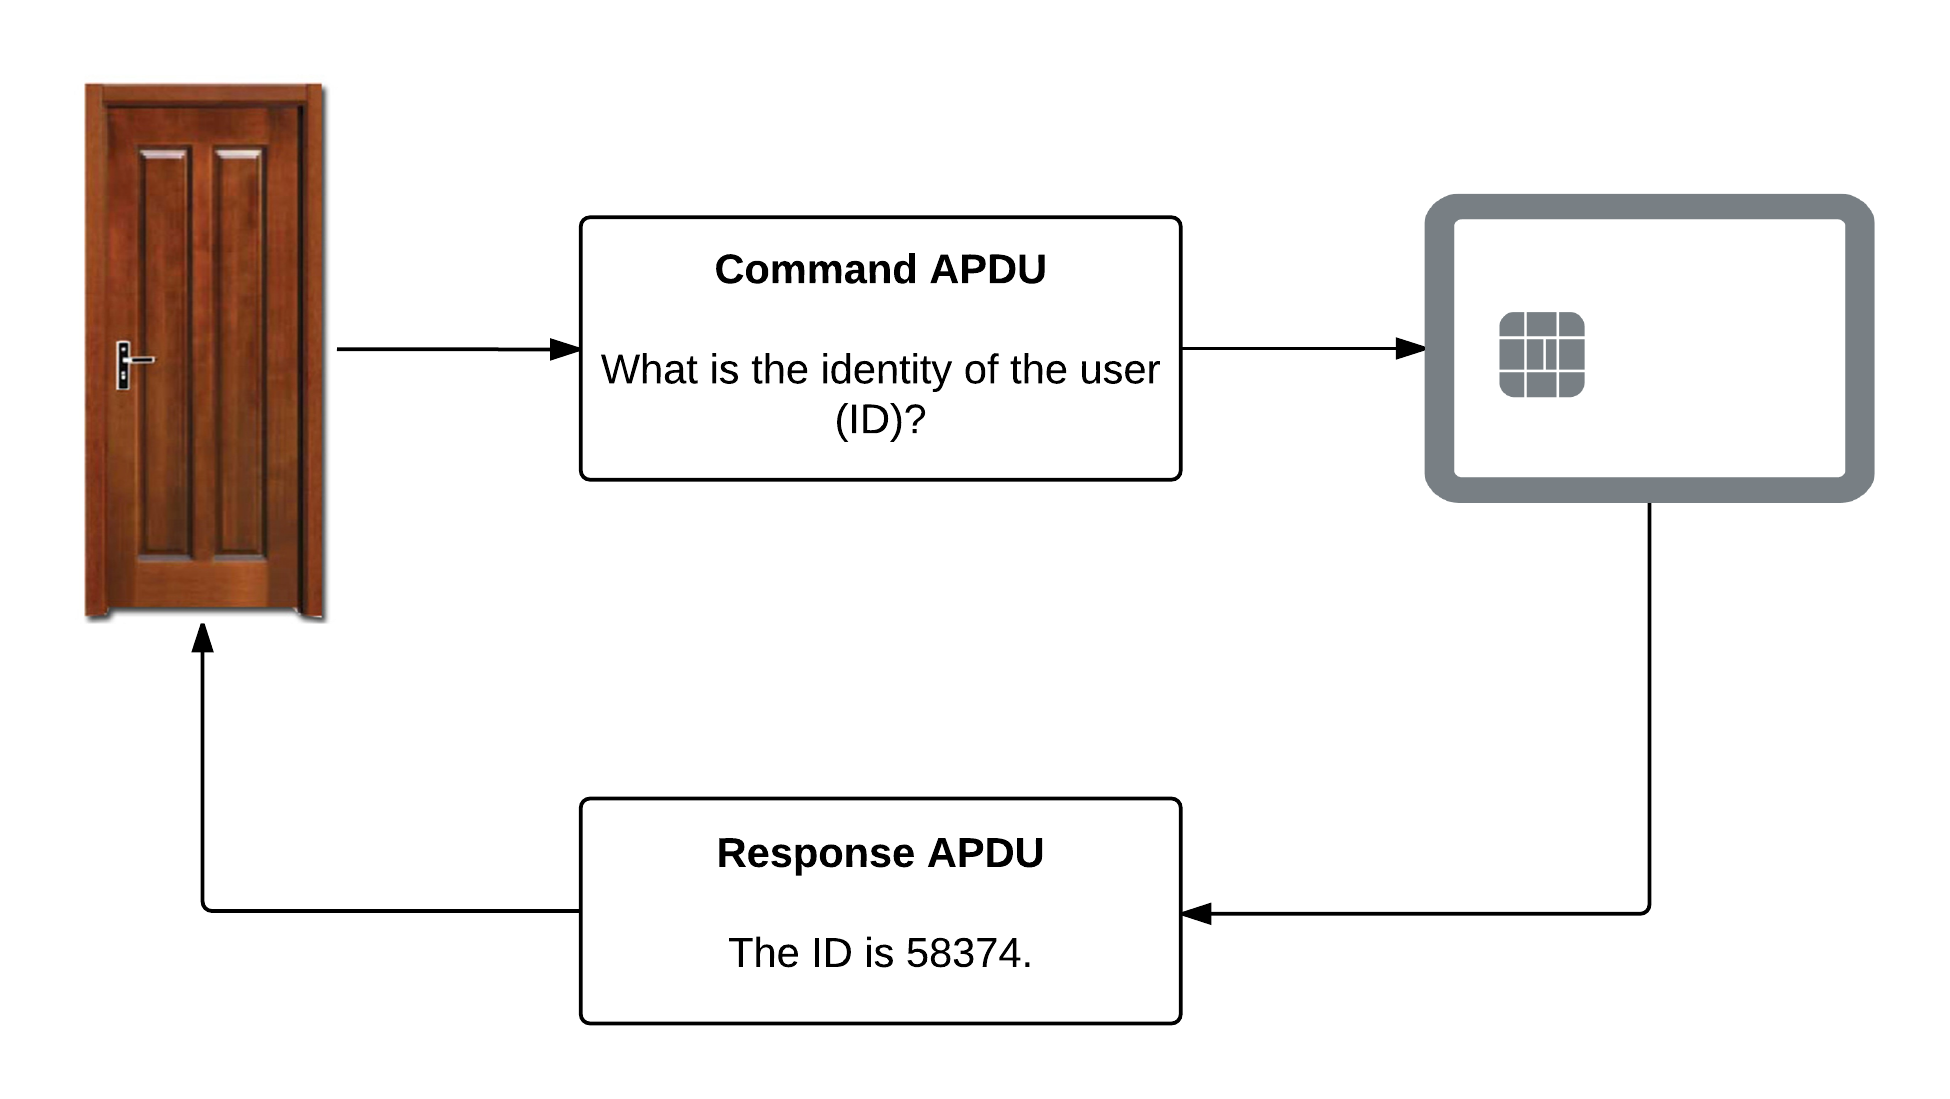
\includegraphics[width=0.95\textwidth]{images/doornfc.png}
\end{figure}

On most smart cards there is an application manager which listen for a special type of Command APDU: a Select APDU. The Select APDU contains information on what type of smart card application a sender is trying to communicate with and the job of the application manager is to activate the correct application. Before communicating with a smart card the sender should send out a Select APDU, if this step is skipped you run the risk of sending information to the wrong smart card application.

\subsection{Java Card programming language}
\label{sec:javacard}
In section \ref{sec:smartcard} we described that smart cards are able to store data as well as process input and output. All smart cards have their own operating system that allows developers to write applications that run on the smart cards. Smart cards are not limited to one applications per card, but are able to have multiple applications installed. Traditionally it was not feasible to create programs that ran on different smart card manufacturer cards as the micro processors were manufacturer specific \cite{javacardapplet}. This created an environment where smart card issuers and their developers were locked to a specific manufacturer.

The company Schlumberger \cite{schlumberger}, later joined by Sun Microsystems \cite{sunMicroSystems}, outlined Java Card 1.0. Java Card were to alleviate the problem of manufacturer specific code and to let developers write generic applications. Newer Java Card version includes a development kit that provides a test environment and a converter tool that prepares the Java Card applet/program for installation onto a smart card. The newest Java Card version is currently 3.0.5 \cite{javacard305}.

The Java Card language behaves very similar to standard Java, but there are some substantial differences. Many Java classes and features are not present, e.g., int, double, long, java.lang.SecurityManager, threading and object cloning \cite{javacardlimits}. The structure of the applets differ from standard Java applets. All Java Card applets must implement:
\begin{itemize}
    \item \texttt{void install (byte [] barray, short bOffset, byte bLength)}
    \item \texttt{void process(APDU apdu)}.
\end{itemize}
\texttt{Install} is invoked when the applet is downloaded onto the smart card and should register and initialize the applet \cite{javacardinstall}. \texttt{Process} is the entry point for all requests to the application and where the applet specific logic is done \cite{javacardprocess}.

Garbage collection in the Java Card language differs from standard Java. In standard Java garbage collection is performed by the Java Virtual Machine (JVM) and runs independently of the application. In Java Card objects are stored in the persistent memory (EEPROM) and writing to this memory is very time-consuming. As a result it was decided that there is no automatic garbage collection in Java Card and that garbage collection must be invoked by the application itself. Deciding when to perform garbage collection is very difficult as on one side you don't want to do it often, and on the other side if you run out of memory you are out of luck.

When incorporating the features of a smart card with a mobile device it would be beneficial to not rely on an external contact card or contactless card. One of the key features of the Java Card language is that the software is able to run on technological different smart cards. As such it is possible to deploy the Java Card applet to special micro SD memory cards. This essentially enables the smart card to be integrated with the mobile device, but at the same time be an external runtime environment. Figure \ref{fig:msdcard} is a micro SD memory card produced by Gemalto.

\begin{figure}[h!]
  \caption{Micro SD card from Gemalto.}
  \label{fig:msdcard}
  \centering
    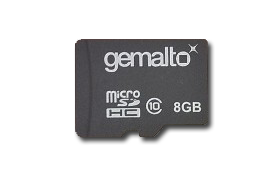
\includegraphics[width=0.75\textwidth]{images/msd.png}
\end{figure}


\subsection{Other smart card programming languages}
There exists several other languages for smart card programming. The two most notable are Java Card (section \ref{sec:javacard}) and MULTOS \cite{multos}. The latter uses the programming language C as the language for writing applications.

\section{Android operating system}
Mobile operating system refers to the operating system running on a mobile device (smartphones, GPS devices, tablets, etc.). In this thesis we will focus mainly on smartphones and tablets since their capabilities are within our scope and the fact that they often share the same operating system. For practical reasons and because of time constraints we have restricted us to one mobile operating system.

Android is an open source licensed mobile operating system and is based on one of the LTS (long-term support) branches of the Linux kernel. Google Inc. \cite{google} is the current developer of the mobile operating system and their primary focus has been smartphones and tablets. In later years Google has put resources into incorporating Android with TVs, wrist watches and cars. In 2015 Q2 82,8 \% of smartphones worldwide was shipped with a version of the Android mobile operating system \cite{androidMarketShare}.

The Android mobile operating system supports applications that are written in Java, GO and C/C++. The applications run in their own sandbox with their own allocated memory space, but applications can also access shared resources given permission to do so by the user.

\section{Cryptography}
%What is cryptography?
Cryptography is a method for protecting confidential data using complex mathematics and computer science. Most cryptographic functions/algorithms relies heavily on the fact that the mathematics are so complex that they are ``uncrackable'' without knowledge of the encryption/decryption key.

\subsection{Public-key cryptography}
\label{sec:publicKeyCrypto}
Public-key cryptography refers to a set of methods for asymmetric cryptography. It is based around the concept that one entity (user, server, etc.) generates a key pair consisting of one public key and one private key. Data encrypted using the public key can only be decrypted by the private key and due to the complexity of the keys it is improbable that the private key can be generated from the public key. The public key, as the name suggests, is publicly available for other entities. This combination allows entities to communicate securely given that they have each others public key and their private key is stored securely. Figure \ref{fig:encrypt_basic} shows how a sender can send a message that only the receiver can read. Although it is important to note that this operation is more resource intensive and time consuming compared to symmetric key encryption/decryption.

\begin{figure}[h!]
  \captionsetup{justification=centering,margin=1.5cm}
  \caption{Asymmetric key encryption/decryption using public-private key pair.}
  \label{fig:encrypt_basic}
  \centering
    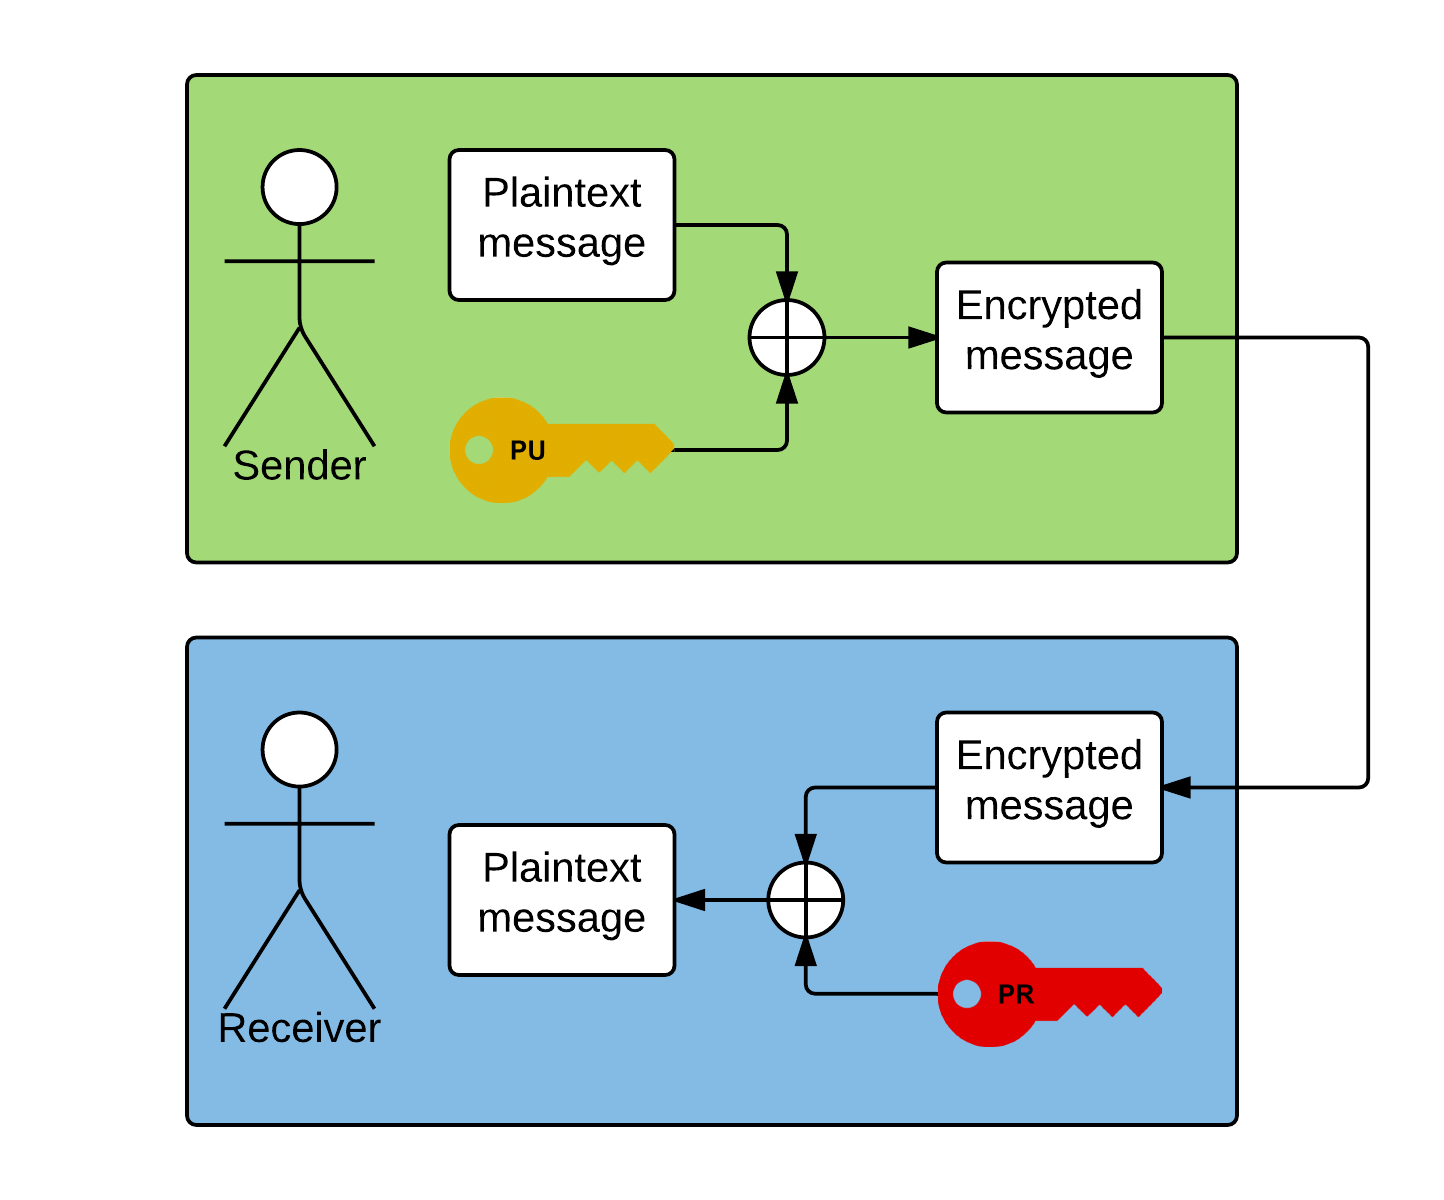
\includegraphics[width=1\textwidth]{images/encrypt_basic.png}
\end{figure}

Message authentication can also be done by public-key cryptography. First the message is hashed using a secure hash function, for instance SHA-2 \cite{shaRFC}, which creates a digest. The digest is then encrypted with the private key and the ``digital signature'' is then sent with the original message. The receiver can then verify the integrity of the message by computing the hash of the message using the same secure hash function and decrypt the ``digital signature'' using the senders public key. If they are a match the receiver can with certainty conclude that the message has not been tampered with and originates from the sender.

\begin{figure}[h!]
  \captionsetup{justification=centering,margin=1.5cm}
  \caption{Digital signing using public-private key pair.}
  \label{fig:signing_basic}
  \centering
    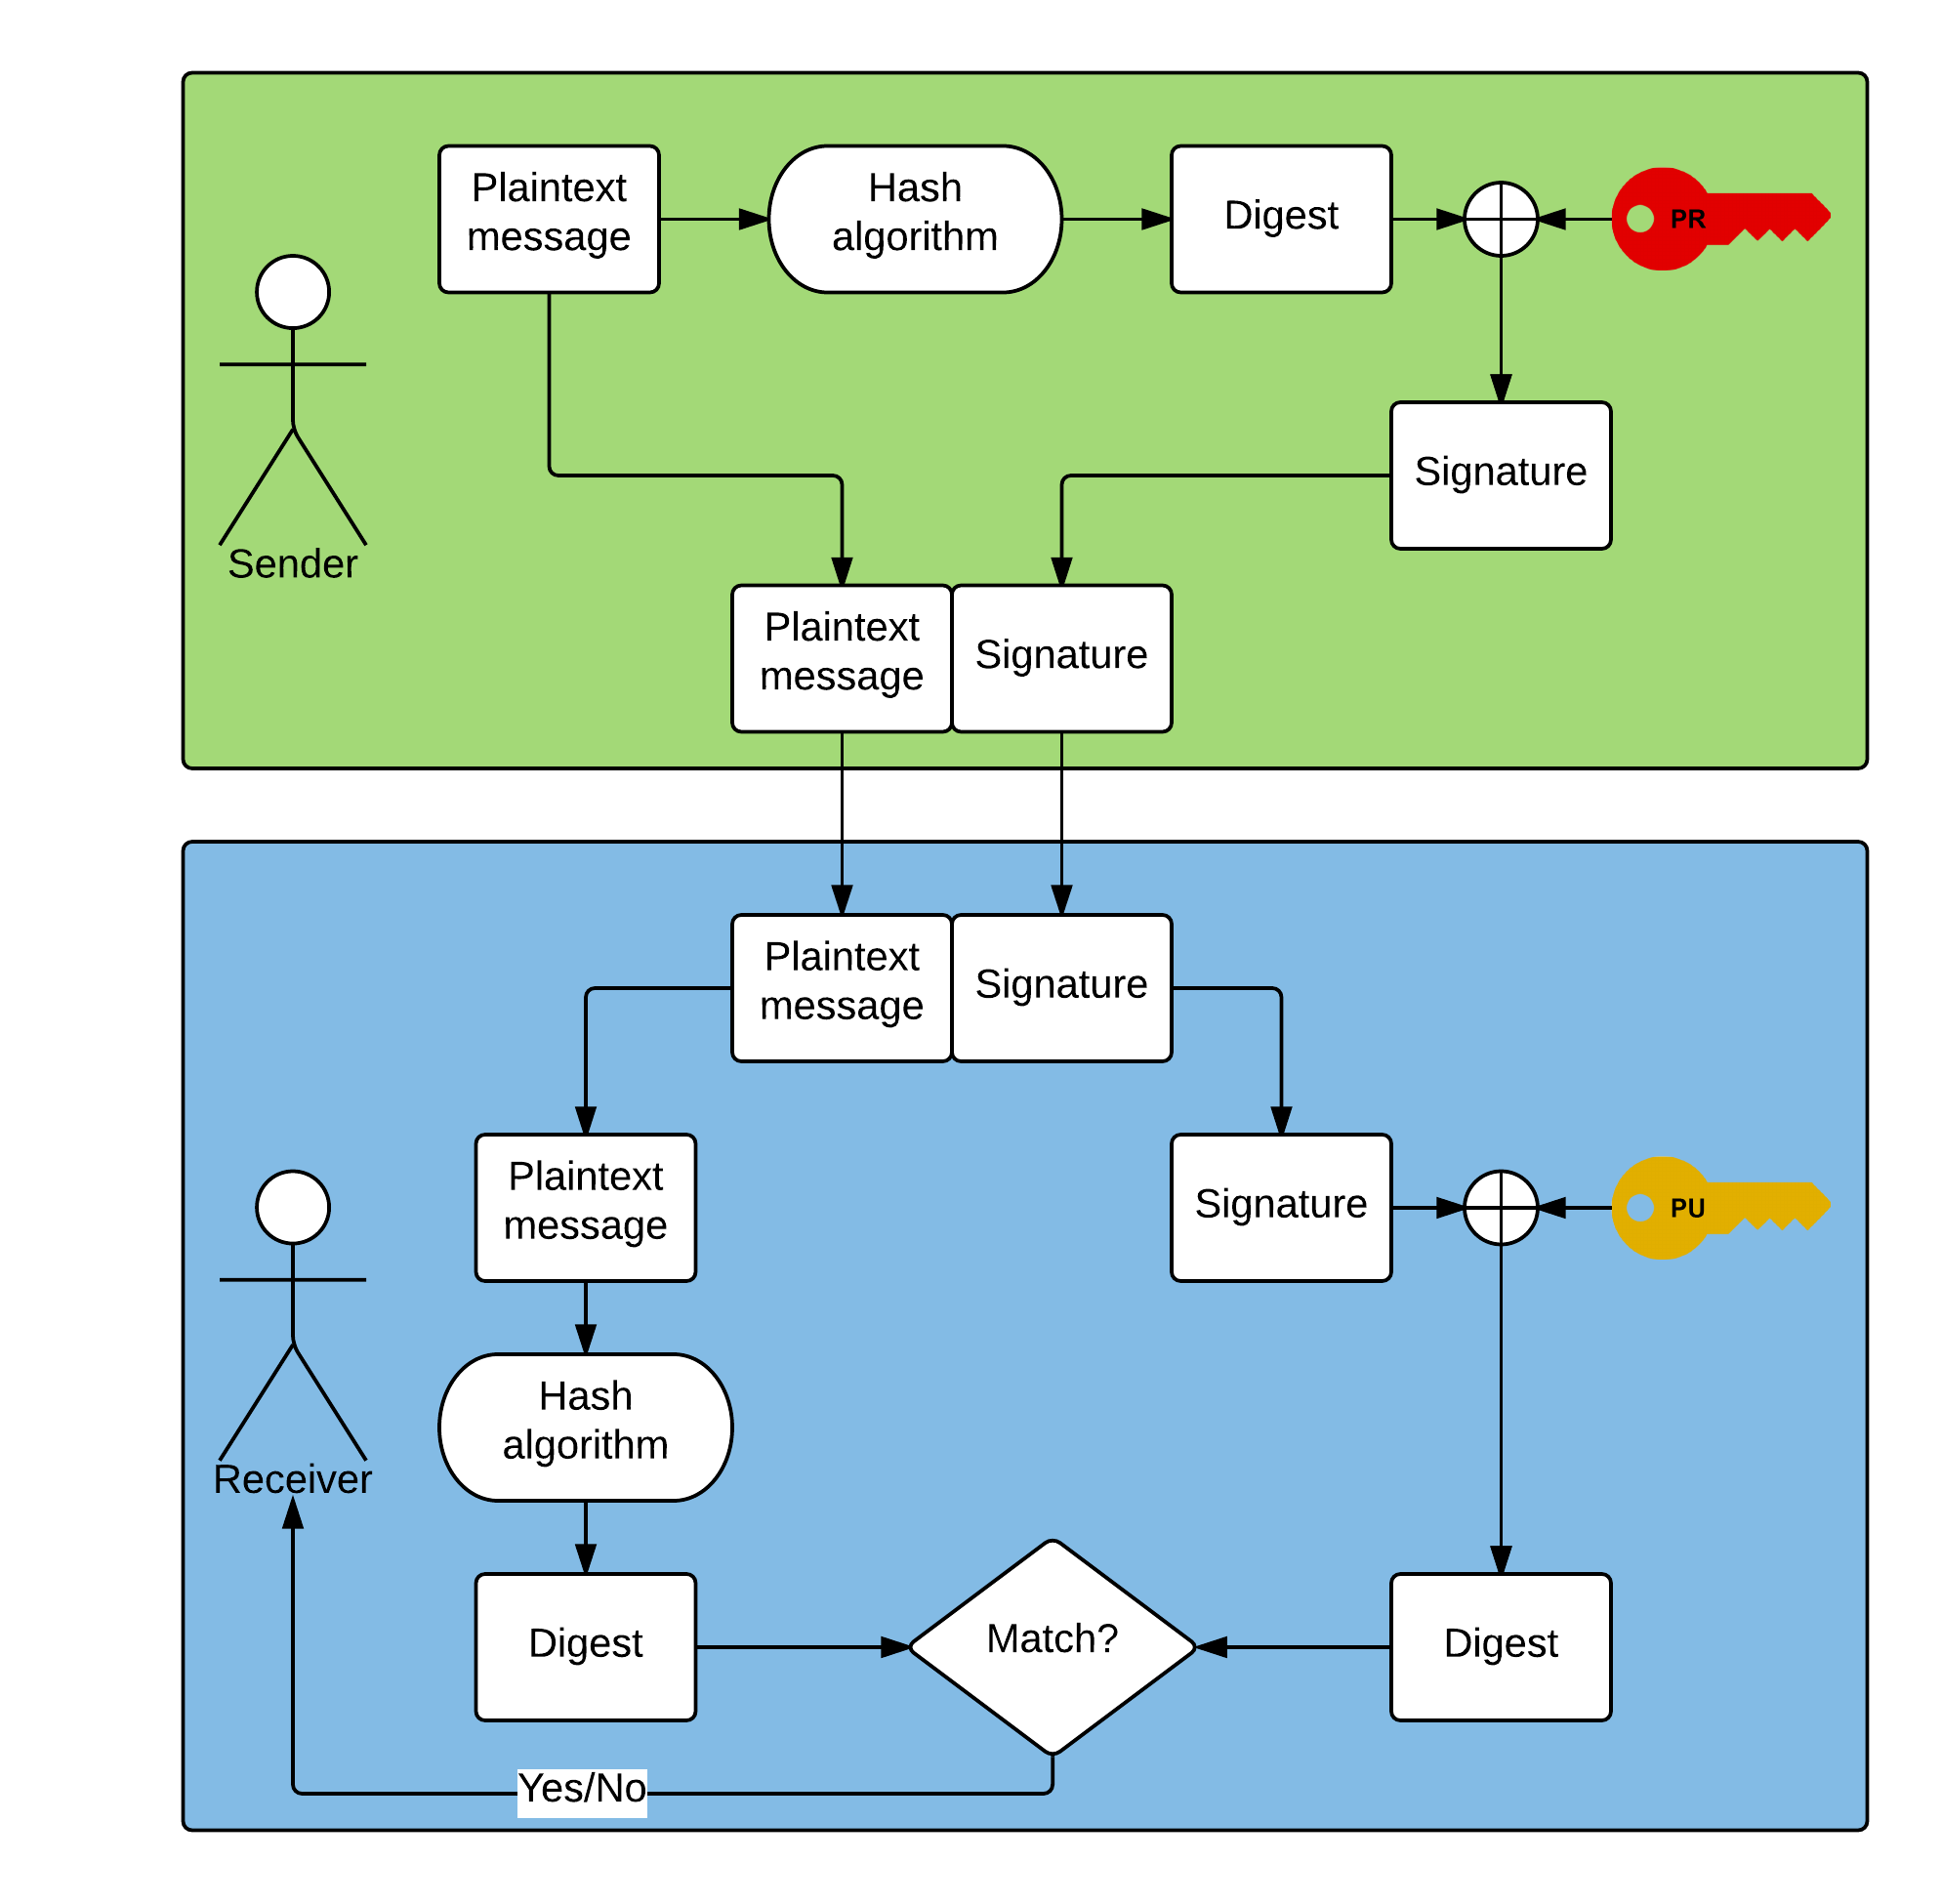
\includegraphics[width=1\textwidth]{images/signing_basic.png}
\end{figure}

\subsection{Symmetric-key cryptography}
Symmetric-key cryptography uses the same cryptographic key for both encryption and decryption. There are two main areas of application for symmetric-key cryptography; secure storage of data and secure communication. Secure storage of data is the most straight forward of the two. An entity (user, server, etc.) generates a key, encrypts the data using the key, stores the key for future use and decrypts the data using the key whenever the entity require the data. As long as the key is stored securely and the encryption algorithm is secure the data can be stored in an unsecured environment. Secure communication using symmetric-key is similar, but instead of the same entity decrypting the data, the encrypted data is transmitted to a new entity which decrypts it using the same key. This requires the key or key generation to be known by both parties, also known as a ``shared secret''. There are two methods for symmetric-key encryption/decryption. Stream ciphering takes one byte at the time and encrypts/decrypts it whereas block ciphering takes bigger chunks of data and encrypts/decrypts the data. Both methods have their own weaknesses and strengths \cite[~Ch. 2.1.1]{cryptoMath}.

Stream ciphering is fast and relatively simplistic to implement. This along with the fact that it can encrypt byte by byte makes it very suitable for use when plaintext data comes in  unknown length and over time (streams). Areas of application includes voice chat, video feed and http communication. Disadvantages of stream ciphering is that if the algorithm is cracked then it is susceptible to insertions and modifications as well as the fact that a single plaintext symbol is represented as a single ciphertext symbol (limited alteration).

Block cipher is a more complex and requires more overhead. First of data must be divided into equal size blocks. The blocks cannot be too small as then they are prone to dictionary attacks and not too big as it will make the encryption/decryption process too resource intensive. In block cipher the block size must be fixed through the encryption process. This will often result in redundant data. For example, 200-bit plaintext with a 64-bit block size will result in three blocks of 64-bit and a fourth block with only 8 bit of ``real'' data and 56 bit of redundant bits. Since block ciphering uses the previous block to cipher the current block it is possible to detect tampering and faults, but this also results that data may be lost if a block becomes corrupt.


\section{Mobile technology vulnerabilities}
Mobile technology vulnerabilities and attack vectors are numerous and before looking into how smart cards can help mitigate an alleviate threats we will need to identify and characterize them.
\subsection{Infected Device}
The most obvious threat to mobile devices is when the mobile device itself is infected with virus or malware. The type of virus or malware can vary, some are harmless and serve more as an annoyance or trying to trick the user into visiting bogus websites, but some are more malicious and will access private files and information. From a security stand-point it is a disaster if a virus or malware is able to read and modify data which is otherwise confidential.

Often the user will not know that their mobile device is infected and some viruses or malware are very hard to detect by anti-virus. The ``2015 Cheetah Mobile Security Report'' \cite{cheetahSec} reports that the number of viruses on Android devices exceeds over 9,5 million and that the problem is growing. When designing and developing applications one should take into consideration that the mobile device may be infected or compromised.


\subsection{Lost or Stolen Device}
An attacker may gain physical access to the users mobile device through theft or simply that the user misplaced the mobile device. With physical access to the device an attacker would be able to retrieve data from the device. A common defense against this is encrypting the data on the device, but this requires the keys to be stored somewhere securely. If the keys are not stored securely the result is that the data on the device may fall into the wrong hands.

\subsection{Insecure Communication Channel}
\label{sec:unsecureCommunication}
Communication is a vital part of modern systems; data is sent between devices and between devices and servers. Sensitive data requires a secure communication channel which cannot be tapped into by a third party. Secure communication on public networks involves agreeing upon encryption keys which the data should be encrypted with before being sent. Encrypting the communication channel will protect against man-in-the-middle attacks, but this requires both parties to authenticate themselves as encrypting the data won't help if you are sending the data directly to the attacker. More on this in section \ref{sec:authenticationChallenges}.

\subsection{Authentication Challenges}
\label{sec:authenticationChallenges}
%Are people who they say the are?
As mentioned in section \ref{sec:unsecureCommunication} a secure communication channel is useless if you are sending the data directly to the attacker. A vital part of communication security is being able to authenticate the parties in a communication transaction. If the attacker is able to impersonate another party by installing fake certificates on the mobile device or by tricking the user into communicating with the attacker the consequences can be of significance.

\subsection{Insecure Applications}
An often overlooked attack vector is badly implemented applications on the mobile device. This may include memory leaks, weak cryptography, open for code injections or openly exposing private data to third parties. In rare cases an application with flaws may expose other applications for attacks, but there exists countermeasures to this, for instance that all applications run in their own sandbox.

  % !TEX root = ../Article.tex
\chapter{Smart card objective}
As mentioned in section \ref{sec:goals} we want to create a framework for easy communication between a mobile device and a smart card. We want to achieve this not only for testing, but to be able to hand over a ready to use framework for any parties interested so that further development and testing may continue.

The framework should lay the very foundation needed for using the mobile device and smart card in a secure fashion. The basic things we want to cover are:
\begin{itemize}
    \item Secure communication
    \item Key management
    \item Basic encryption
\end{itemize}
If we manage to create a framework covering these three points we believe that we have a great starting point for further testing and development.

\section{Design goals}
\label{sec:designAndroidGoals}
The design goals for the framework are:

\begin{itemize}
    \item Easy to use.
    \item Require little to no understanding of JavaCard or smart cards.
    \item Extendable.
\end{itemize}

Even though most users of our framework will have a basic understanding of smart cards we believe that abstracting some central concepts will make the framework easier to use. One of the concepts we make abstract is APDU. As a user/developer of the framework you can choose not to work with APDUs and use pre-created methods.

As we cannot possibly predict all types of uses for the framework we will also include a method for sending custom commands to the smart cards. This ensures that developers don't feel limited in how they can use the framework as well as catering to advanced users. More on the implemented methods in section \ref{sec:androidApp}.

\section{Smart card application}
The first part of the framework is the application on the smart card.

\subsection{Java Card version}
The cards we have supports java card 2.2.2 and this is the version we will target. A natural question is "Why don't we target java card 3 and above?". Smart cards used for banking or handling other highly confidential data needs to be evaluated under the Common Criteria \cite[Ch.~26.3.2]{securityEngineering} standards. Potentionally we may handle confidential data and as a result we want smart cards with a Evaluation Assurance Level (EAL) 4 or above. Achieving EAL4 or above is an expensive and long process and the relatively few products have this certification. The micro SD card we have access to are certified with EAL5+, but only supports java card 2.2.2 \cite{gemaltoidgo8030}.

%TODO EAL list
\begin{table}[h!]
\caption{Evaluation Assurance Level}
\label{tbl:EAL}
\centering

    \begin{tabular}{ | c | l |}
        \hline
        \thead{Level}
        & \thead{Description} \\ \hline

        1 & Functionally Tested \\ \hline
        2 & Structurally Tested \\ \hline
        3 & Methodically Tested and Checked \\ \hline
        4 & Methodically Designed, Tested and Reviewed \\ \hline
        5 & Semiformally Designed and Tested \\ \hline
        6 & Semiformally Verified Design and Tested \\ \hline
        7 & Formally Verified Design and Tested \\ \hline

    \end{tabular}
\end{table}

%TODO beskriv table

A natural question we need to ask ourselves is: "Do we want Java card 3?"



\subsection{Development environment}
In order to develop applications for the smart cards we will be using Eclipse 3.2 with java development kit version 1.6.45. In order to develop smart card applications more easily we will use the Eclipse-JCDE plugin \cite{eclipseJCDE} which provides a virtual runtime environment along with build tools. Even though Eclipse 3.2 is severely outdated it provides the tools necessary to do the job.

\begin{figure}[h!]
  \caption{Screenshot of Eclipse showing JavaCard tools.}
  \label{fig:eclipse}
  \centering
    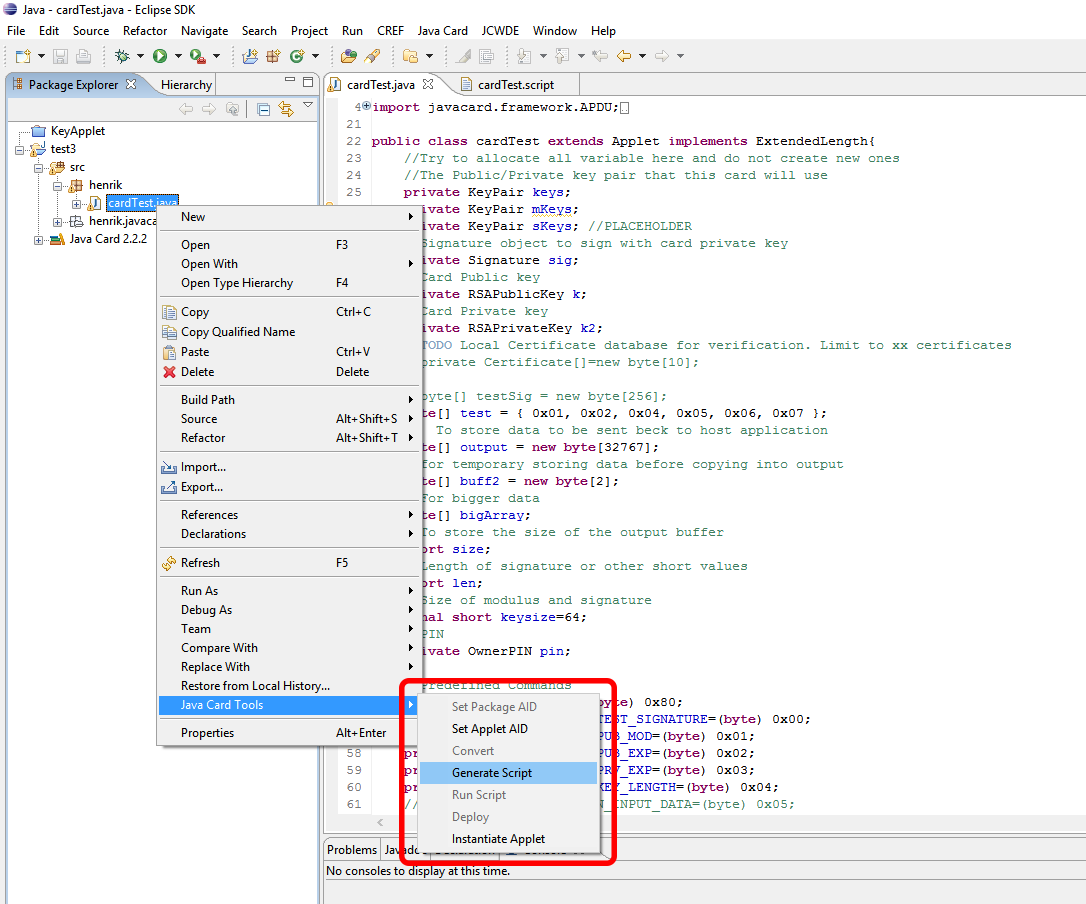
\includegraphics[width=0.95\textwidth]{images/eclipse.png}
\end{figure}

In figure \ref{fig:eclipse} we can see the tools for generating the deployable smart card application package. The screenshot also shows how the editor looks like any other Eclipse version. Even though this version of Eclipse includes tools for sending and receiving APDUs to the application (testing), we have decided not to use these tools as they proved themselves to be unstable and not representative of real world use. This is mostly due to the fact that the application is deployed to an emulator and does not have \textit{any} hardware limitations of a physical smart card.

\subsection{Deployment}
We will be using GlobalPlatformPro (GP) \cite{globalplatform} to deploy and manage applets on the physical smart cards. GP is a command line tool and is compatible with our hybrid Gemalto card with reader as well as the micro SD card. There are three essential steps when deploying an application to a smart card:

\begin{itemize}
    \item Delete the smart card application along with the stored data.
    \item Delete the smart card package.
    \item Install the new smart card.
\end{itemize}

To do this we will utilize a simple batch script which consisting of three lines of code (listing \ref{lst:batchInstall}). To gain access to the cards we need to provide a key set by the manufacturer. This requirement is added as an added security measure to verify that developers are supposed to have write access to the smart cards. Lastly we supply the AID we wish to use for our application. It is important to note that the AID must be unique and the installation will not succeed if the AID is in use.

\begin{lstlisting}[language=batch,caption=Install and deploy script for GlobalPlatformPro., label=lst:batchInstall,escapechar=!]
    gp.exe -visa2 -key !\%!KEY!\%! -delete !\%!AID!\%!
    gp.exe -visa2 -key !\%!KEY!\%! -delete !\%!PACKAGEID!\%!
    gp.exe -visa2 -key !\%!KEY!\%! -install !\%!PATH!\%! -d
\end{lstlisting}

\subsection{Basic testing environment}
To test the smart card application that is deployed on the physical cards (without going through an Android application) we will be using pyApduTool \cite{pyapdutool}. pyApduTool is a tool for sending APDUs to a smart card through a card reader or memory card reader and lets us observe how the card behave when receiving and transmitting data.

\begin{figure}[h!]
  \caption{Select APDU sent to smart card via PyApduTool}
  \label{fig:pyapdutool}
  \centering
    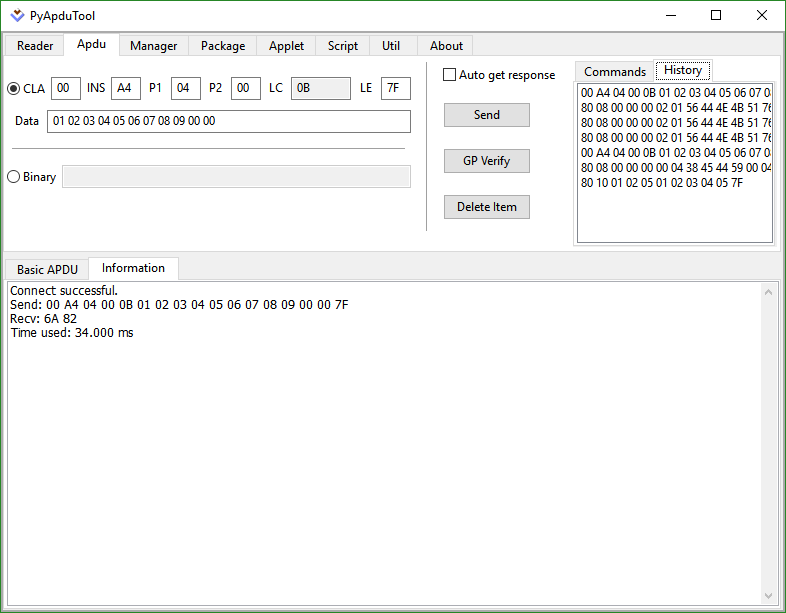
\includegraphics[width=0.95\textwidth]{images/pyapdutool.png}
\end{figure}

PyApduTool does not support extended APDU and this limits us to a high degree when testing our smart card application. Testing through PyApduTool does not test mobile device behaviour such as out of memory, too much traffic or NFC limitations. After the initial basic testing PyApduTool became obsolete and we had to test via an Android application.

\subsection{Application}
\paragraph{Goal}\mbox{}\\
The goal of the smart card application was to create an autonomous and easy to extend platform for future tests. This resulted in an application split into three parts.

\paragraph{Initialization}\mbox{}\\
As described in section \ref{sec:javacard} all javacard applications must implement the method \texttt{Install}. \texttt{Install} invokes the constructor of the smart card and this is where all variables that need initialization are initialized. For instance if the smart card application needs to generate keys or random numbers this is where it is done as the constructor will be invoked only once. All buffers that needs to be used should also be initialized here to avoid allocating memory everytime the application is used.

\paragraph{Data processing}\mbox{}\\
In the mandatory \texttt{Process} method (refer to section \ref{sec:javacard}) all data processing takes place. First a built in method in the javacard API, \texttt{selectingApplet()}, is invoked. This method checks if the incoming APDU is a SELECT APDU and acts accordingly. If the incoming APDU is not a SELECT APDU the incoming APDU is copied to a new buffer for easier data manipulation. Next we use a switch statement switching over the second byte, INS, to determine which instruction we want to perform. After processing the data and performing the work we want to do (sign data, encrypt, etc.) we copy our response to the outgoing buffer.

\paragraph{Finalization}\mbox{}\\
At the end of the \texttt{Process} invokation we invoke the \texttt{Send} method which takes the data in the outgoing buffer, package it for sending and send it as a response APDU.

\paragraph{The result}\mbox{}\\
What we end up with is a test plattform where we are only concerned with declaring variables, initializing variables and writing code for the specific test case. Listing \ref{lst:pseudoCard} shows pseudocode for the java card application with the extendable areas highlighted.


\begin{lstlisting}[caption=Pseudo code for javacard test application., label=lst:pseudoCard,escapechar=!]
public class cardApplication extends Applet implements ExtendedLength{

    !\colorbox{highlight}{//Variable declarations}!

    private cardApplication() {
    	!\colorbox{highlight}{//Variable initialization}!
    }

    public void process(APDU apdu) {
    	//Process incoming APDU
        if (selectingApplet()) {
			return;
		}
        buff = apdu.getBuffer();

    	switch(buff[ISO7816.OFFSET_INS]){
            case 0x00:
            case 0x01:
            !\colorbox{highlight}{...}!
            case 0xff:
            default:

    	}
    	Send(apdu);
    }

    private void send(APDU apdu) {
    	//Package outgoing buffer
    	//Send response APDU
    }
}
\end{lstlisting}

As seen in \ref{lst:pseudoCard} we allow for 256 cases/uses of the smart card, but if we include the use of P1 and P2 from section \ref{sec:communicationstandard} there are in theory 256\textsuperscript{3} = 16777216 possible cases. This does not include the pre-implemented methods which are explained in section \ref{sec:androidApp}. Their counterparts in the smart card application have the following byte values:

\begin{itemize}
    \item byte SEND\_U\_PUB\_MOD = (byte) 0x01;
    \item byte SEND\_U\_PUB\_EXP = (byte) 0x02;
    \item byte SIGN = (byte) 0x03;
    \item byte BINDING = (byte) 0x05;
    \item byte RSACRYPTO = (byte) 0x06;
    \item byte AESCRYPTO = (byte) 0x09;
\end{itemize}

We will not go into detail on how the individual cases are built up. Refer to Appendix A for JavaCard code.

\section{Android application}
\subsection{IDE}
Android Studio \cite{androidIDE} is the official IDE for Android application development. Android Studio is based on IntelliJ IDEA \cite{intelliJIDEA} and provides many automated tools for building, packaging and publishing Android applications.
\subsection{3rd party libraries}
As mentioned in section \ref{sec:equipment} Gemalto provides a java library, IDGo800, for using their smart cards.

\begin{aquote}{Gemalto.com \cite{GemaltoIDGo800}}
"IDGo 800 for Mobiles is a cryptographic middleware that supports the Gemalto IDPrime cards and Secure Elements on Mobile platforms: Contact and contactless smart cards, MicroSD cards, UICC-SIM cards, embedded Secure Elements (eSE) and Trusted Execution Environment (TEE)."
\end{aquote}

The part of IDGo800 SDK we are interested in is very small and enables us to send custom APDUs to micro SD smart cards.

We will be using the "android.nfc" package in order to communicate with NFC smart cards. This package is included in the standard Android SDK which in turns means that all Android devices with a NFC reader and minimum API level 9 \cite{androidNFCminSDK} can use our library.

\subsection{Application}
\label{sec:androidApp}

In section \ref{sec:designAndroidGoals} we described the goals of the framework. The first goal we will describe the implementation of is "extendable" or in other words, being able to send custom APDUs. Explaining how this is implemented will give a better understanding of how the framework is built up and makes it easier to understand the pre-implemented methods.

We used the same approach on the Android application as on the smart card application; an autonomous and easy to extend plattform for tests. This resulted in a new library, "smartcardlibrary",  which sole purpose is to transmit APDUs as easily as possible along with some basic functionality.

\paragraph{Custom APDUs}\mbox{}\\
To send custom APDUs to a smart card,\texttt{CommunicationController} must be instantiated and the application must know the application identifier of the smart card application. Further the current activity must implement\\ \texttt{NfCSmartcardControllerInterface} or \texttt{MSDSmartcardControllerInterface} (depending on smart card type) in order to be notified when the transaction is complete. Before continuing one will need to call the methods \texttt{setupNFCController} or \texttt{setupmSDController} depending on the smart card. Listing \ref{lst:NFCLibraryExample} shows an example implementation on how an activity may utilize the library for sending custom commands to a NFC smart card.

\begin{lstlisting}[caption=Java code example showing how to send and receive commands to a NFC smart card., label=lst:NFCLibraryExample,escapechar=å]

public class PayloadActivity extends AppCompatActivity
    implements NFCSmartcardControllerInterface {
    CommunicationController cc = new CommunicationController();
    ...

    private void initNFCCommunication(){


        String AID = "0102030405060708090007";
        String hexMessage = "95404F3FB1";
        String INS = "06";
        String p1 = "00";
        String p2 = "00";
        cc.setupNFCController(this, this);
        cc.initNFCCommunication(AID, INS, p1, p2, hexMessage);
    }

    å@Overrideå
    public void nfcCallback(final String completionStatus){
        if(!completionStatus.equals("OK")){
            return;
        }
        StorageHandler stHandler =
            new StorageHandler(getApplicationContext());
        String response =
            stHandler.readFromFileAppDir(
                FilePaths.tempStorageFileName
            );
    }
}

\end{lstlisting}

In order for the library to perform an asyncronous transaction the library will temporary save the responses from the cards to a file only accessible by the running application. To retrive the data the current activity should use the included \texttt{StorageHandler} class as used in listing \ref{lst:NFCLibraryExample}. The library also provides the class, \texttt{Converter}, for converting between Strings, hex and byte arrays.

\paragraph{Pre-implemented methods}\mbox{}\\
Recall the areas we want to cover from the beginning of the chapter. The functionality we have implemented so far are:

\begin{itemize}
    \item Bind smart card to mobile device.
    \item Encrypt/decrypt data using RSA key on card.
    \item Encrypt/decrypt data using AES key on card.
    \item Get public key of the smart card.
    \item Sign data using the public key of the smart card.
\end{itemize}

To use these functionalities one would only need to create an Android \texttt{Activity}, invoke either \texttt{setupNFCController(...)} or \texttt{setupmSDController(...)} (depending on smart card), and utilize the desired methods.
The methods available are:

\begin{itemize}
    \item public void disableNFC(...)
    \item public void bindingStepOne(...)
    \item public void bindingStepTwo(...)
    \item public void bindingStepThree(...)
    \item public void signData(...)
    \item public void cryptoRSA(...)
    \item public void cryptoAES(...)
    \item public void getCardPubMod(...)
    \item public void getCardPubExp(...)
\end{itemize}
The binding process is designed in three steps. First step is to ask the smart card if it requires a PIN-code and how many attempts are left. Second step requires a PIN-code and if this is correct the smart card application will move on to step three. The last step is sending the public key of the mobile device and getting the verification package from section \ref{sec:proposedSolution}. More discussion on this matter in section \ref{sec:bindingcardandphone}.

The rest of the methods should be self-explanatory and one should refer to the javadoc in Appendix A for parameter requirements and pre-conditions.

Figure \ref{fig:package} shows how the library is structured and the entry point for applications is through the packages:

\begin{itemize}
    \item com.master.henrik.controller
    \item com.master.henrik.statics
    \item com.master.henrik.shared
\end{itemize}

%TODO UPDATE

\begin{figure}[h!]
  \caption{Library package diagram.}
  \label{fig:package}
  \centering
    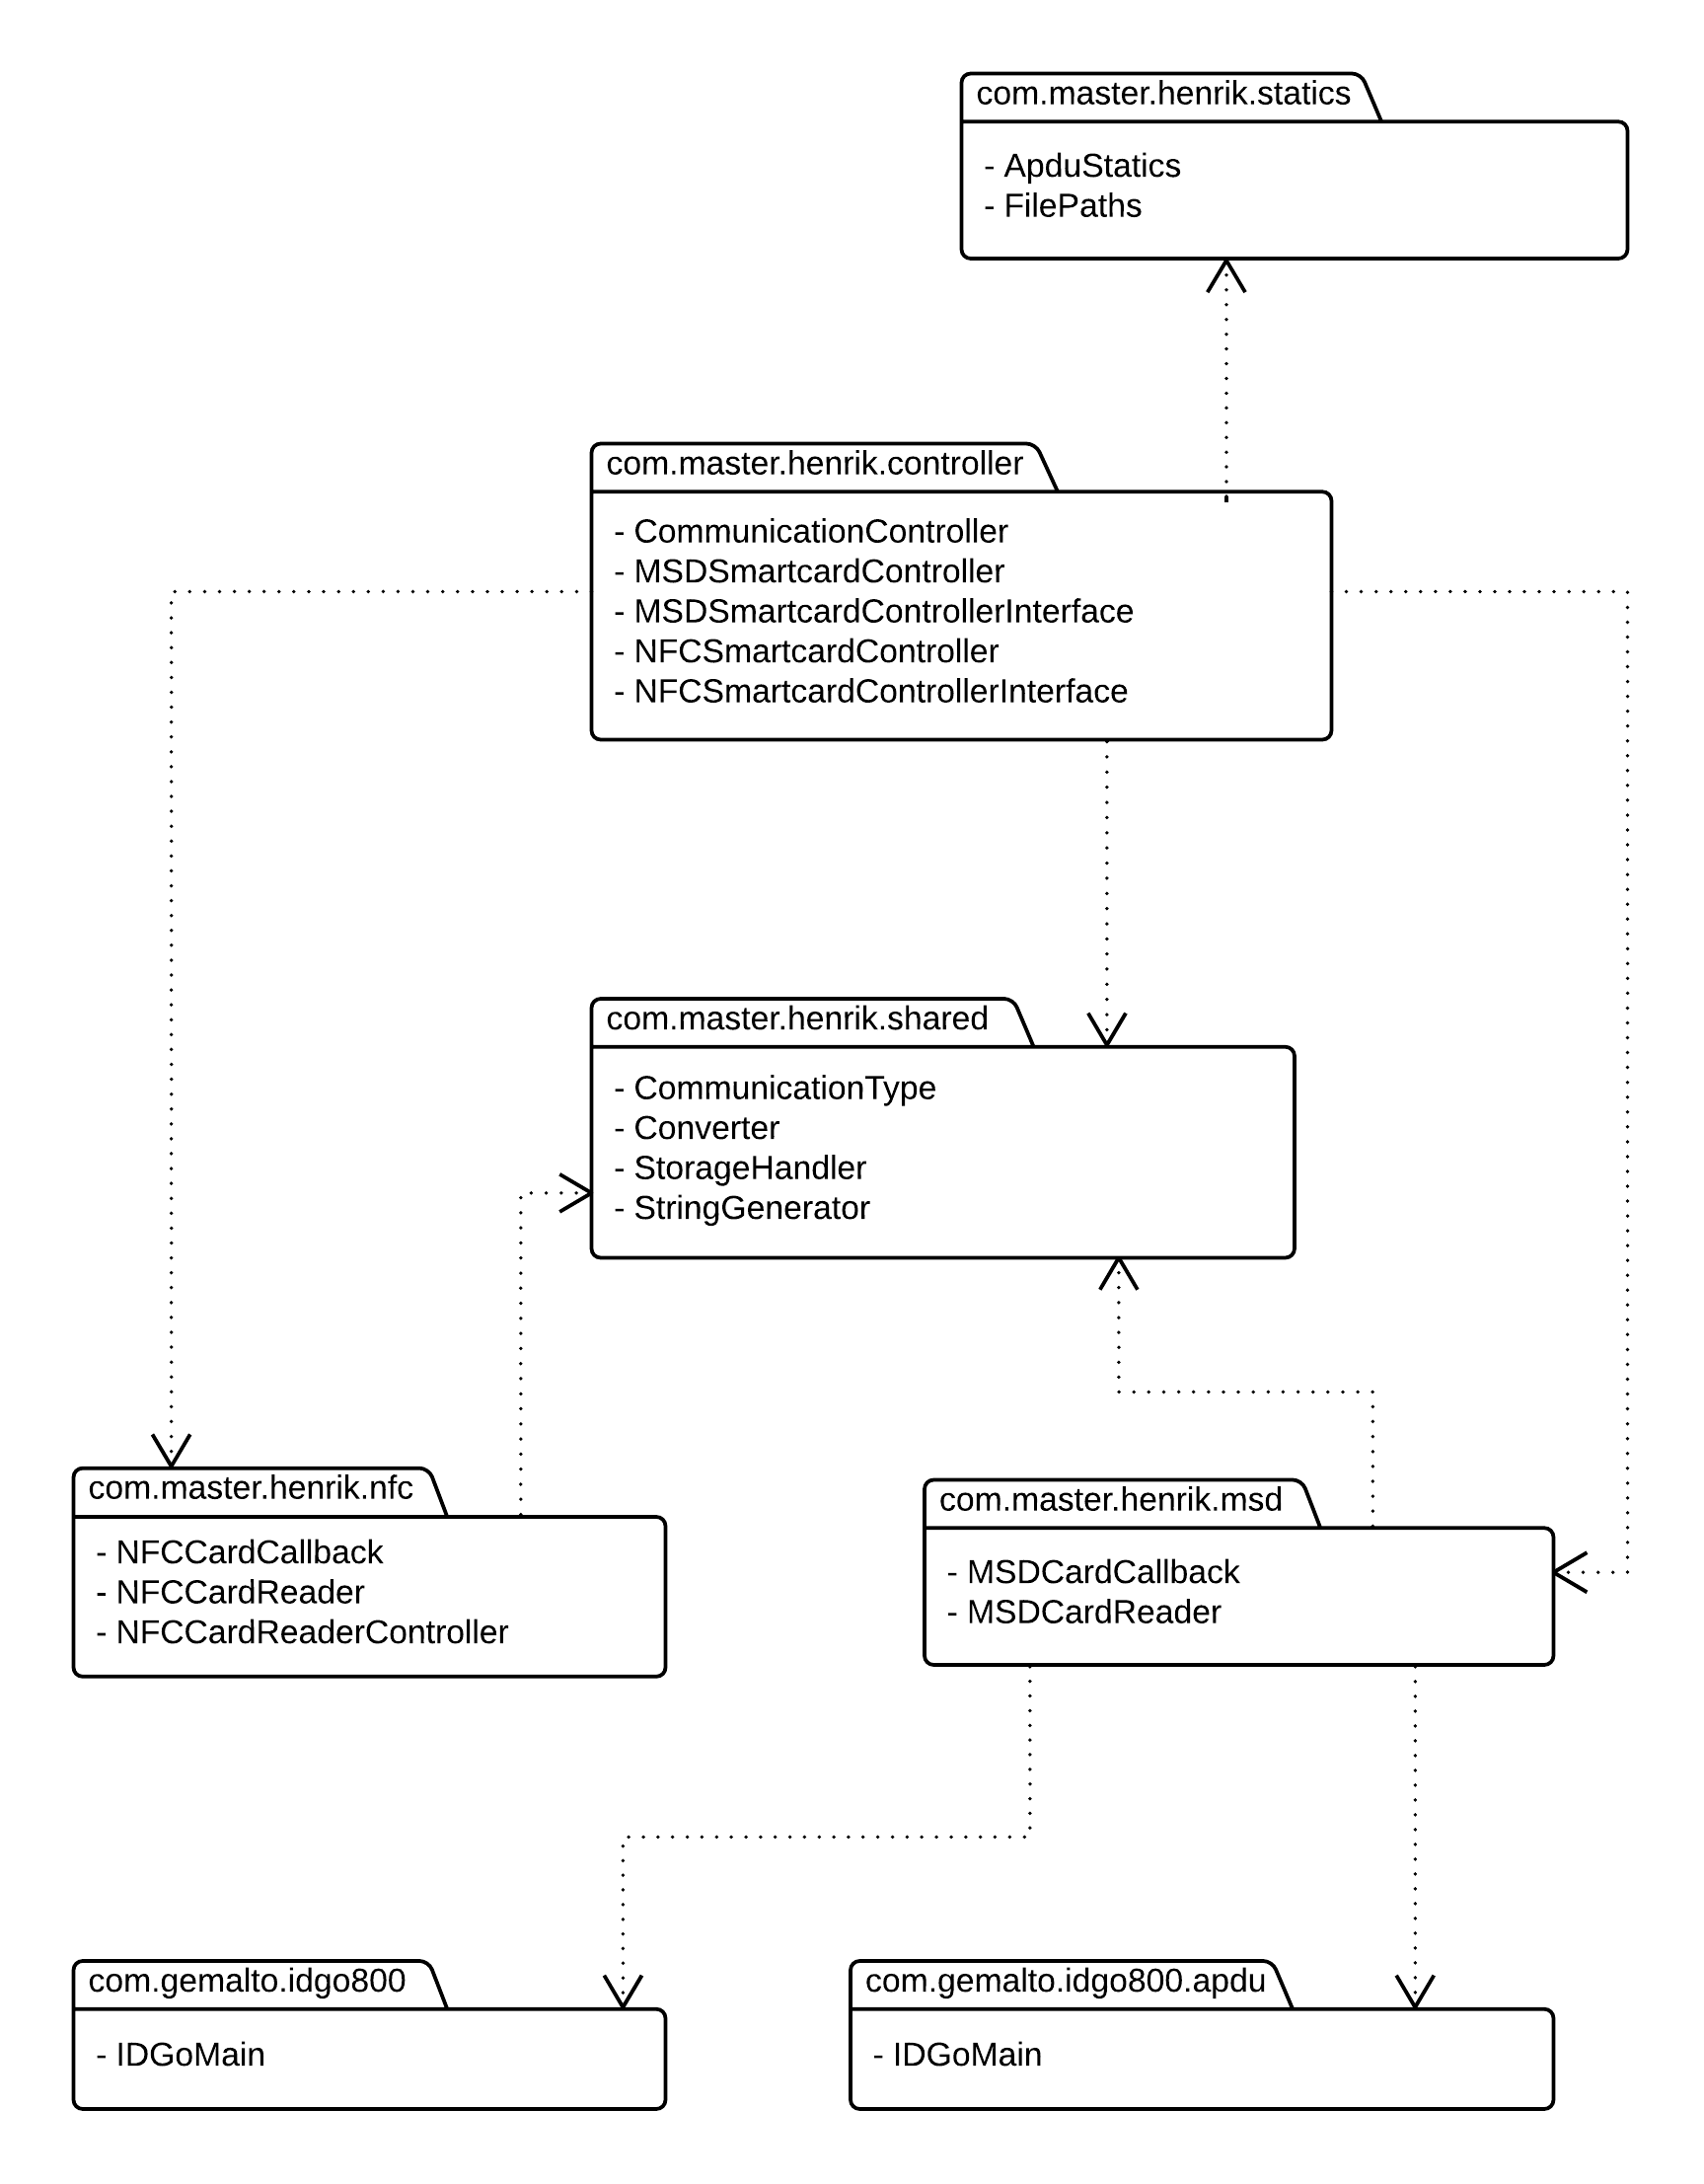
\includegraphics[width=0.95\textwidth]{images/package2.png}
\end{figure}

  %% !TEX root = ../Article.tex
\chapter{Mobile threats}
Mobile threats and attack vectors are numerous and before looking into if smart cards can help mitigate or alleviate we will need to identify and characterize them.
\section{Infected device}
The most obvious threat to mobile devices is when the mobile device itself is infected with virus or malware. The type of virus or malware can vary, some are harmless and serve more as an annoyance or trying to trick the user into visiting bogus websites, but some are more malicious and will access private files and information. From a security stand-point it is a disaster if a virus or malware is able to read and modify data which is otherwise confidential.

Often the user will not know that their mobile device is infected and some viruses or malware are very hard to detect by anti-virus. The ``2015 Cheetah Mobile Security Report'' \cite{cheetahSec} reports that the number of viruses on Android devices exceeds over 9,5 million and that the problem is growing. Taking into concideration that the mobile device we are operating on may be infected is of the utmost importance when designing and developing applications.

\section{Lost or stolen device}
An attacker may gain physical access to the users mobile device through theft or simply that the user misplaced the mobile device. With physical access to the device an attacker would be able to retrive data from the device. A common defence against this is encrypting the data on the device, but this requires the keys to be stored somewhere securely. If the keys are not stored securely the result is that the data on the device will fall into the wrong hands.

\section{Unsecure communication channel}
\label{sec:unsecureCommunication}
Communication is a vital part of modern systems; data is sent between devices and between devices and servers. Sensitive data requires a secure communication channel which cannot be tapped into by a third party. Secure communication on public networks involves agreeing upon encryption keys which the data should be encrypted with before being sent. Encrypting the communication channel will protect against man-in-the-middle attacks, but this requires both parties to authenticate themselves as encrypting the data won't help if you are sending the data directly to the attacker. More on this in section \ref{sec:authenticationChallenges}.

\section{Authentication challenges}
\label{sec:authenticationChallenges}
%Are people who they say the are?
As mentioned in section \ref{sec:unsecureCommunication} a secure communication channel is useless if you are sending the data directly to the attacker. A vital part of security is being able to authenticate the parties in a transaction. If the attacker is able to impersonate another party by installing fake certificates on the mobile device or by tricking the user into communicating with the attacker the consequences can be of significance.

\section{Unsecure applications}
An often overlooked attack vector is badly implemented applications on the mobile device. This may include memory leaks, weak cryptography, open for code injections and plainly exposing private data to third parties. In rare cases an application with flaws may expose other applications for attacks, but there exists countermeasures to this, for instance that all applications run in their own sandbox.
 moved to background
  % !TEX root = ../Article.tex
\chapter{Challenges and use cases}
\label{ch:challenges}
In this chapter we will analyze some of the challenges one will face when trying to use smart cards to enhance the security of Android mobile devices. In chapter 2 we covered the attack vectors and vulnerabilities that exists on the mobile device platform and we believe that smart cards can help mitigate them. We have established that smart cards are able to run critical operations in a secure and closed execution environment along with the fact that they are tamper resistant. As a result they are perfectly suited to generate and store cryptographic keys, perform cryptographic operations such as verifying signature or encrypt sensitive data, or enforce strong access control through PIN codes.

On the other hand, smart cards have limited computational power and memory, they are passive elements meaning that they cannot initiate an operation and rely on external commands, as well as the fact that they are not ``aware of the outside world'' except for pre-installed information or the information they receive.

Based on these characteristics we have identified two main areas of use where smart cards can be used to mitigate threats on the mobile device platform:
\begin{enumerate}
  \item Generate and store cryptographic keys to mitigate the threat of a stolen or lost device. Mobile devices that stores cryptographic keys without using smart cards or secure elements are prone to key theft via operating system exploits or weak user passwords.
  \item Use the smart card as a separate trusted operating system that can securely handle the communication with off-card and off-device services and enforce simple security policies. As it is a separate execution environment, this can be achieved even if the mobile device operating system is compromised.
\end{enumerate}

However, in order to ensure that these proposed areas of use function as intended, we will need to overcome some obstacles. First off we will need to establish a trust relationship between the mobile device and smart card in order to verify that they are meant to cooperate and lock/bind them to each other. In section \ref{sec:bindingcardandphone} we elaborate and investigate this challenge. Secondly we will need to define how smart cards and mobile devices handle the encryption keys needed for a secure solution. With this challenge the best we can do is to have a ``best effort approach'', meaning that we have to trust that the solutions provided by the mobile platform are properly implemented. Section \ref{sec:mobileDeviceKeys} investigates this problem. Lastly, we describe how policy enforcement might function using smart cards in section \ref{sec:policies}.

In the next chapter we will perform tests related to the proposed solutions. Even though we were not able to fully implement and test all aspects, we still chose to outline how they can be solved.

%In this chapter we will examine what challenges there are with regards to mobile devices and smart cards co-operating. The challenges must be viewed from a use case perspective where the benefits do not come from solving the challenges, but rather what we are able to achieve afterwards. For each challenge we will provide problem description, motivation, key concepts, possible solution and describe possible attack vectors.
\section{Binding card and mobile device}
\label{sec:bindingcardandphone}
\subsection{Problem description}
%One of the key challenges when utilizing smart cards with mobile devices is establishing an initial trust relationship. How can the mobile device know that it communicates with a certified smart card (company/department issued) and how can the smart card know that it is interracting with a trusted user on a mobile device? To initialize this trust relationship we need to perform a handshake where we verify that all concerning parties can authenticate and authorize each other.
One of the key challenges when utilizing smart cards with mobile devices is establishing an initial trust relationship. How can the mobile device know that it communicates with a certified smart card (company/department issued) and how can the smart card know that it is interacting with a trusted user on a mobile device? The biggest problem of the binding process is that the smart card must trust the mobile device, as we have no way of knowing if we are binding to a compromised mobile device.  If the mobile device is not initially compromised and we are able to use the smart card as a bootstrap for trust, then the direct result is that we can use smart cards as a policy enforcement point (PEP) and secure key storage/generation. To initialize this trust relationship we need to perform a handshake where we verify that all concerning parties can authenticate and authorize each other.

Binding the mobile device and smart card mainly protects against offline attacks where the attacker tries to access resources on the mobile device or smart card independently of each other. For instance if the attacker tries to use the smart card and it's stored keys with another device.

\subsection{Goals}
By binding the smart card and phone together we wish to ensure that a smart card can only be paired with one mobile device and that we are in full control during the process. If we achieve this, then:
\begin{itemize}
  \item The keys stored on the smart card cannot be retrieved or be used on a different mobile device.
  \item Our application on the mobile device cannot be used without the smart card that was paired with our mobile device.
  \item If the binding is successful we may be able to detect if the mobile device becomes compromised on a later point and react to it (delete keys on card, block communication, etc.).
\end{itemize}

This will mitigate vulnerabilities such as:
\begin{itemize}
  \item Lost or stolen device.
  \item Unsecure communication channels.
  \item Authentication challenges.
\end{itemize}

\subsection{Key concepts}
To authenticate the two parties, smart card and mobile device, we will need a third party which they both trust. We introduce a new party, the authority, which acts as a trusted third party. The authority issues the smart cards and employ the users. A direct consequence is that they both trust the authority, otherwise we have no starting point. Since they both trust the authority they can ask the authority to verify the other party as shown in figure \ref{fig:standardAuth}.

\begin{figure}[h!]
  \captionsetup{justification=centering,margin=1.5cm}
  \caption{Using a third party (Authority) to establish a trust relationship between two parties (Application and smart card) lacking trust.}
  \label{fig:standardAuth}
  \centering
    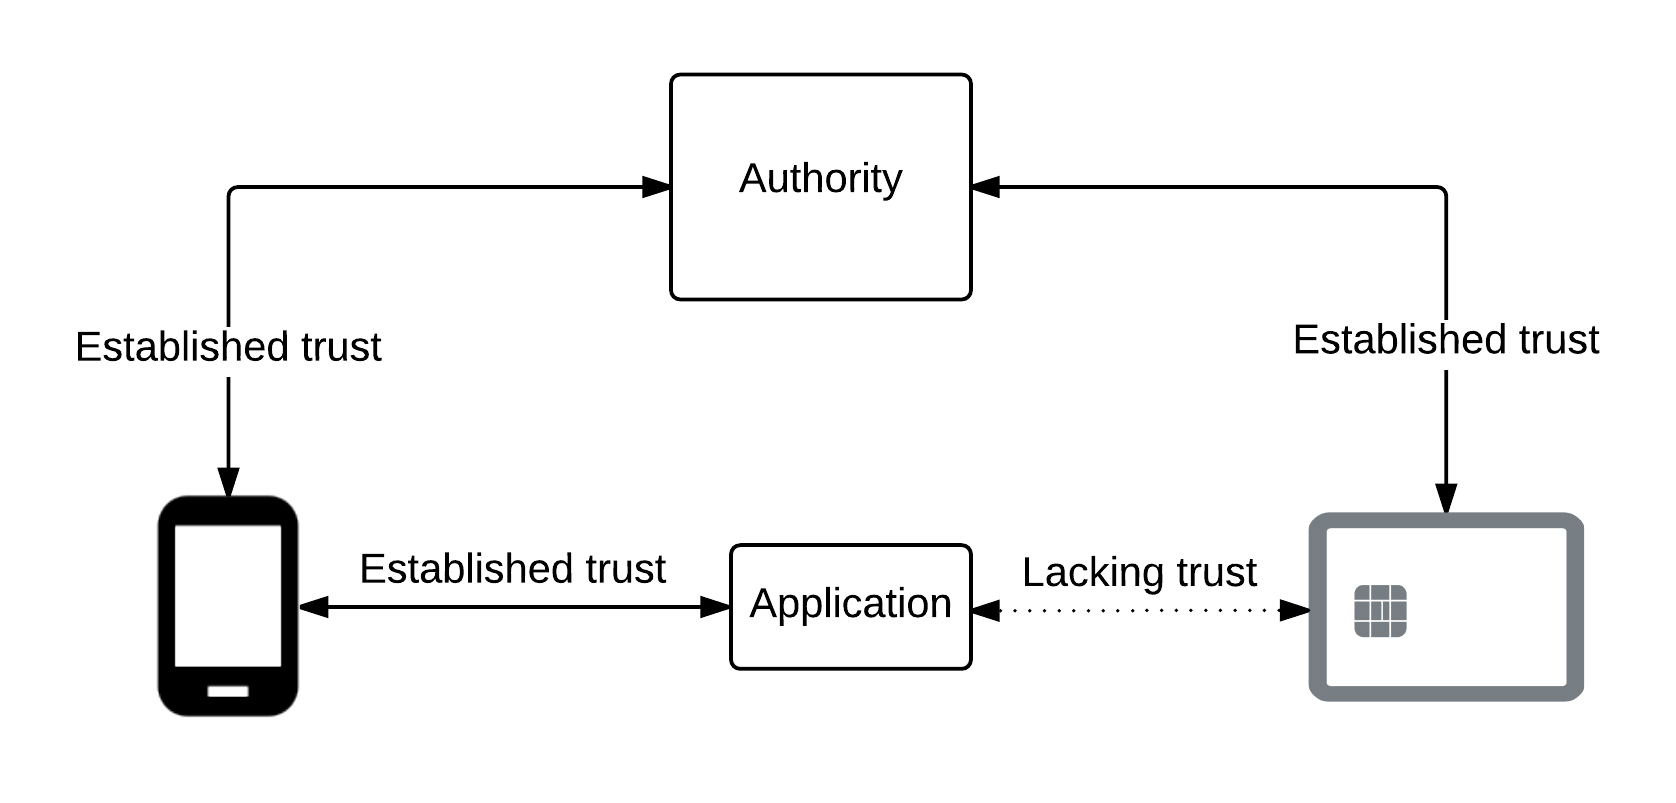
\includegraphics[width=0.95\textwidth]{images/standardAuth2.png}
\end{figure}

One thing that differentiates our challenge from traditional authentication challenges is that the smart card is not able to communicate directly with a trusted third party. All communication from our smart card to off card applications or third parties must go through a mobile device. A technical illustration of this relationship can be seen in figure \ref{fig:smu} where the authority is represented as a server. This drawback introduces a new problem which we have to consider. How do we know if the mobile device relays information between the server and smart card correctly in the authentication process?

\begin{figure}[h!]
  \captionsetup{justification=centering,margin=1.5cm}
  \caption{Server, mobile device and smart card communication flow.}
  \label{fig:smu}
  \centering
    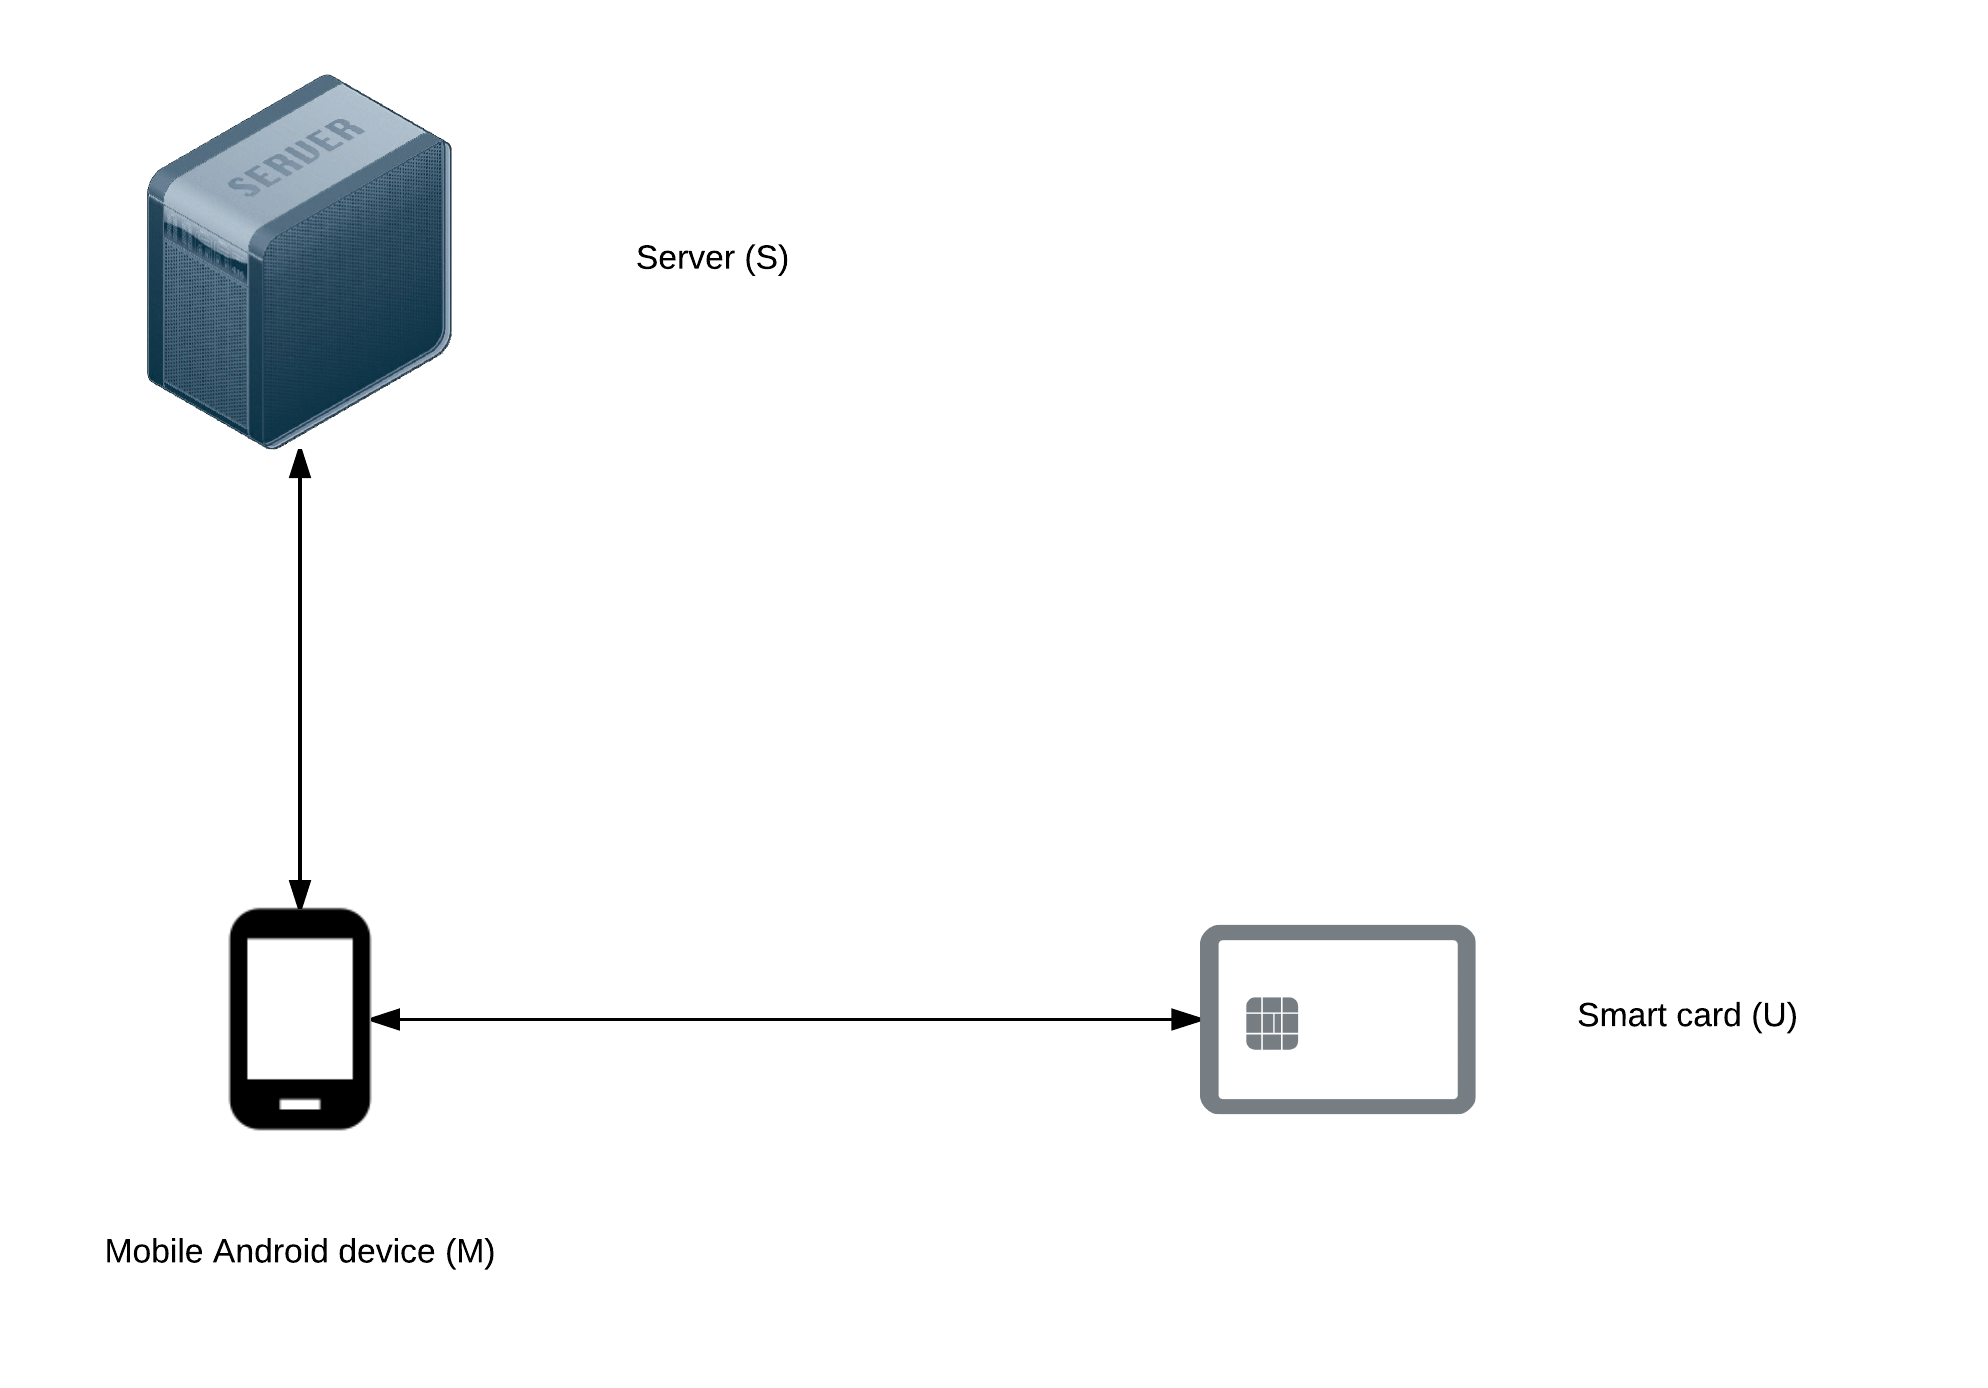
\includegraphics[width=0.95\textwidth]{images/SMU.png}
\end{figure}

To address that all information flowing from the smart card has to go through a possibly compromised mobile device, we can utilize the fact that the authority we are trying to communicate with is also the smart card issuer. What this means is that we can pre-install the authority certificate and public key on the smart card as well as retrieve the public key of the smart card before handing the smart card to the user/employee. In other words, the authority and the smart card have already exchanged all necessary information to securely authenticate each other before deployment.

The mobile device will also need to authenticate with the authority so that the smart card can trust the mobile device. In this process we will need to make some assumptions. The first problem is that we need to  ensure that the mobile device communicates with the right server (authority). By hardcoding the server URL in the mobile device application and making sure that the user installs the right application on his device we can mitigate this threat. To make sure that the user installs the right application we need a secure distribution platform. By using Google Play as distribution platform, we can minimize the risk that the user will download a rogue application with the same name \cite{googlePlaySecureDist}. To further mitigate the risk of installing the wrong application the user can disable the ability to side-load applications and avoid using a rooted device.

%The other attack vector on the mobile device and user is man-in-the-middle attacks.
Another possible attack we should defend against, is man-in-the-middle attacks between the application and the server. If we assume that the user was able to download the correct application we will need to secure the communication channel. To secure the channel we will need to use Transport Layer Security (TLS) \cite{rfc793} which also provides us with protection from replay attacks \cite[~Ch. 9.2.2]{TLS101}. The only downside by using TLS in our case is that we will need the server certificate to verify the server. Traditionally we will need to either pre-install certificates on the mobile device (makes ``bring your own device'' more difficult) or register with a certificate authority (depend on third party). In our case the server certificate is already on the smart card and we can install it on the mobile device. If the mobile device is compromised the certificate may not be used at all or replaced by a malicious certificate. This can be done as the smart card has no control over the mobile device. However, as we describe later, we encrypt some particular data with the public key of the authority on the smart card, and we are thus not prone to man-in-the-middle attacks since the attack cannot decrypt it.

Further we will need the user to authenticate with the authority. We have two options in order to achieve this. First option is that users use a username and password combination directly with the authority, but considering the binding is normally a one time case a more simplified process may be to hand out a one time code along with the smart card. One could also look into distributing one time codes through e-mail or a text message (SMS).

The second option is that the user inputs a PIN to the smart card and if the pin code is correct the smart card can verify that the user is the user he claims to be. This option requires very little overhead and saves a lot of resources in that regard. The problem with this approach is that if the mobile device is already compromised the PIN code may be stolen before the user is able to bind the mobile device with the smart card. If the PIN is a PIN the user regularly uses an attacker may also be able to get the information from the user via other means (social engineering, key loggers, etc.). A one time PIN (OTP) may be a better option than a PIN although this does add more overhead to the process.

The final requirement for the binding process, is that we have a cryptographic mechanism that in practice binds the mobile device and smart card together. We define the binding process to be done when both parties have the public key of each other and have verified that the keys they have are in fact the keys of the two parties. When this is completed, the mobile device and smart card can mutually authenticate each other before initiating any transaction involving sensitive data.

We have described how the parties can authenticate each other, but we will need to describe this as a unified process (refer to section \ref{sec:proposedSolution}) and identify attack vectors and weaknesses (refer to section \ref{sec:attackVectors}).

\subsection{Proposed solution}
\label{sec:proposedSolution}

\paragraph{Pre-conditions}\mbox{}\\
The authority issues the smart cards and administrates the server. During the setup of the smart card the public key and certificate of the server must be installed on the smart card. The public key of the smart card must also be extracted and stored on the server. This creates a base for all future processes.

\paragraph{Verification package}\mbox{}\\
A verification package is a package containing all the information a third party server needs to authenticate the smart card and mobile device. First the mobile device public key and the generated AES key is signed by the smart card. Then we encrypt the package with the public key of the third party server. Figure \ref{fig:h0} visualizes this structure.

\newpage

\begin{figure}[h!]
  \caption{Verification package structure.}
  \label{fig:h0}
  \centering
    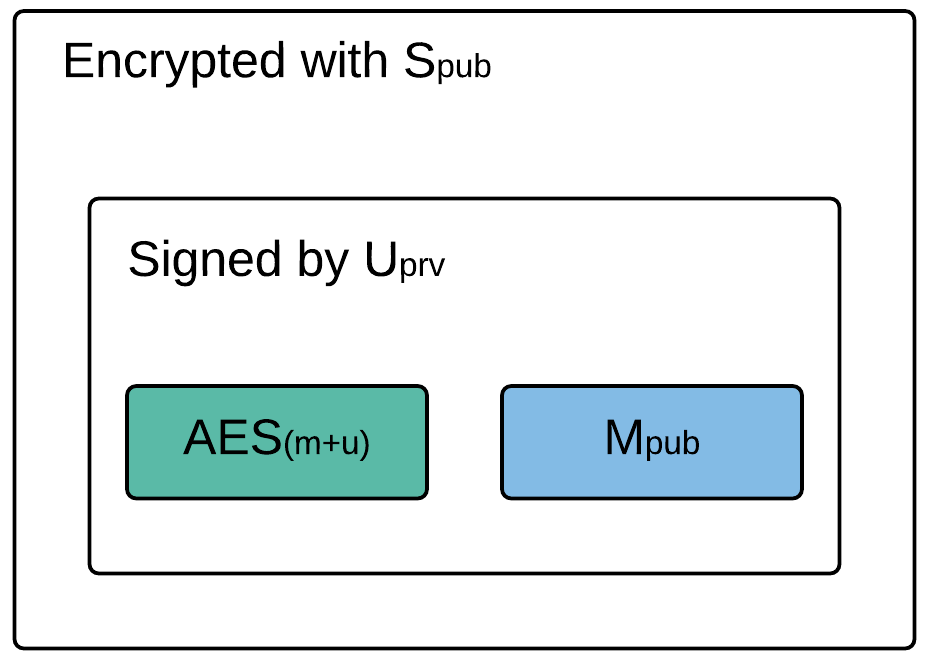
\includegraphics[width=0.95\textwidth]{images/H0.png}
\end{figure}

We propose the following protocol for binding mobile devices and smart cards:

\paragraph{Abbreviations}\mbox{}\\
U - Users smart card \\
M - Mobile device \\
S - Server, representation of authority \\
H\textsubscript{0} - Verification package \\
\{Entity\}\textsubscript{pub} - Public key of an entity (U, M, S)\\
\{Entity\}\textsubscript{prv} - Private key of an entity (U, M, S)\\
\{AES\}\textsubscript{Entity+Entity} - AES key of two entities (U, M, S)\\


\begin{enumerate}
  \item Install the (correct) Android application the on mobile device (M) and insert smart card (U).
  \item M generates RSA key-pair and stores it securely on the device.
  \item M sends M\textsubscript{pub} to U and requests verification package (H\textsubscript{0}) from (U).
  \item U asks for a PIN/OTP.
  \item M provides PIN/OTP.
  \item U generates H\textsubscript{0} (refer to figure \ref{fig:h0}) and sends it to M.
  \item M connects (URL is either hardcoded into application or from certificate) to the server (S) via TLS and sends (H\textsubscript{0}) to S.
  \item S decrypts (H\textsubscript{0}) using S\textsubscript{prv} and verifies the signature of U.
  \item If everything is ok then S saves AES\textsubscript{(M+U)} for safekeeping, signs M\textsubscript{pub} and sends the signed  M\textsubscript{pub} to M.
  \item M forwards the signed M\textsubscript{pub} to U.
  \item U verifies that M\textsubscript{pub} was signed by S and if successful U sends U\textsubscript{pub} to M.
\end{enumerate}

\clearpage
\begin{figure}[h!]
  \captionsetup{justification=centering,margin=1.5cm}
  \caption{Sequence diagram for binding mobile device with smart card.}
  \label{fig:sqd}
  \centering
    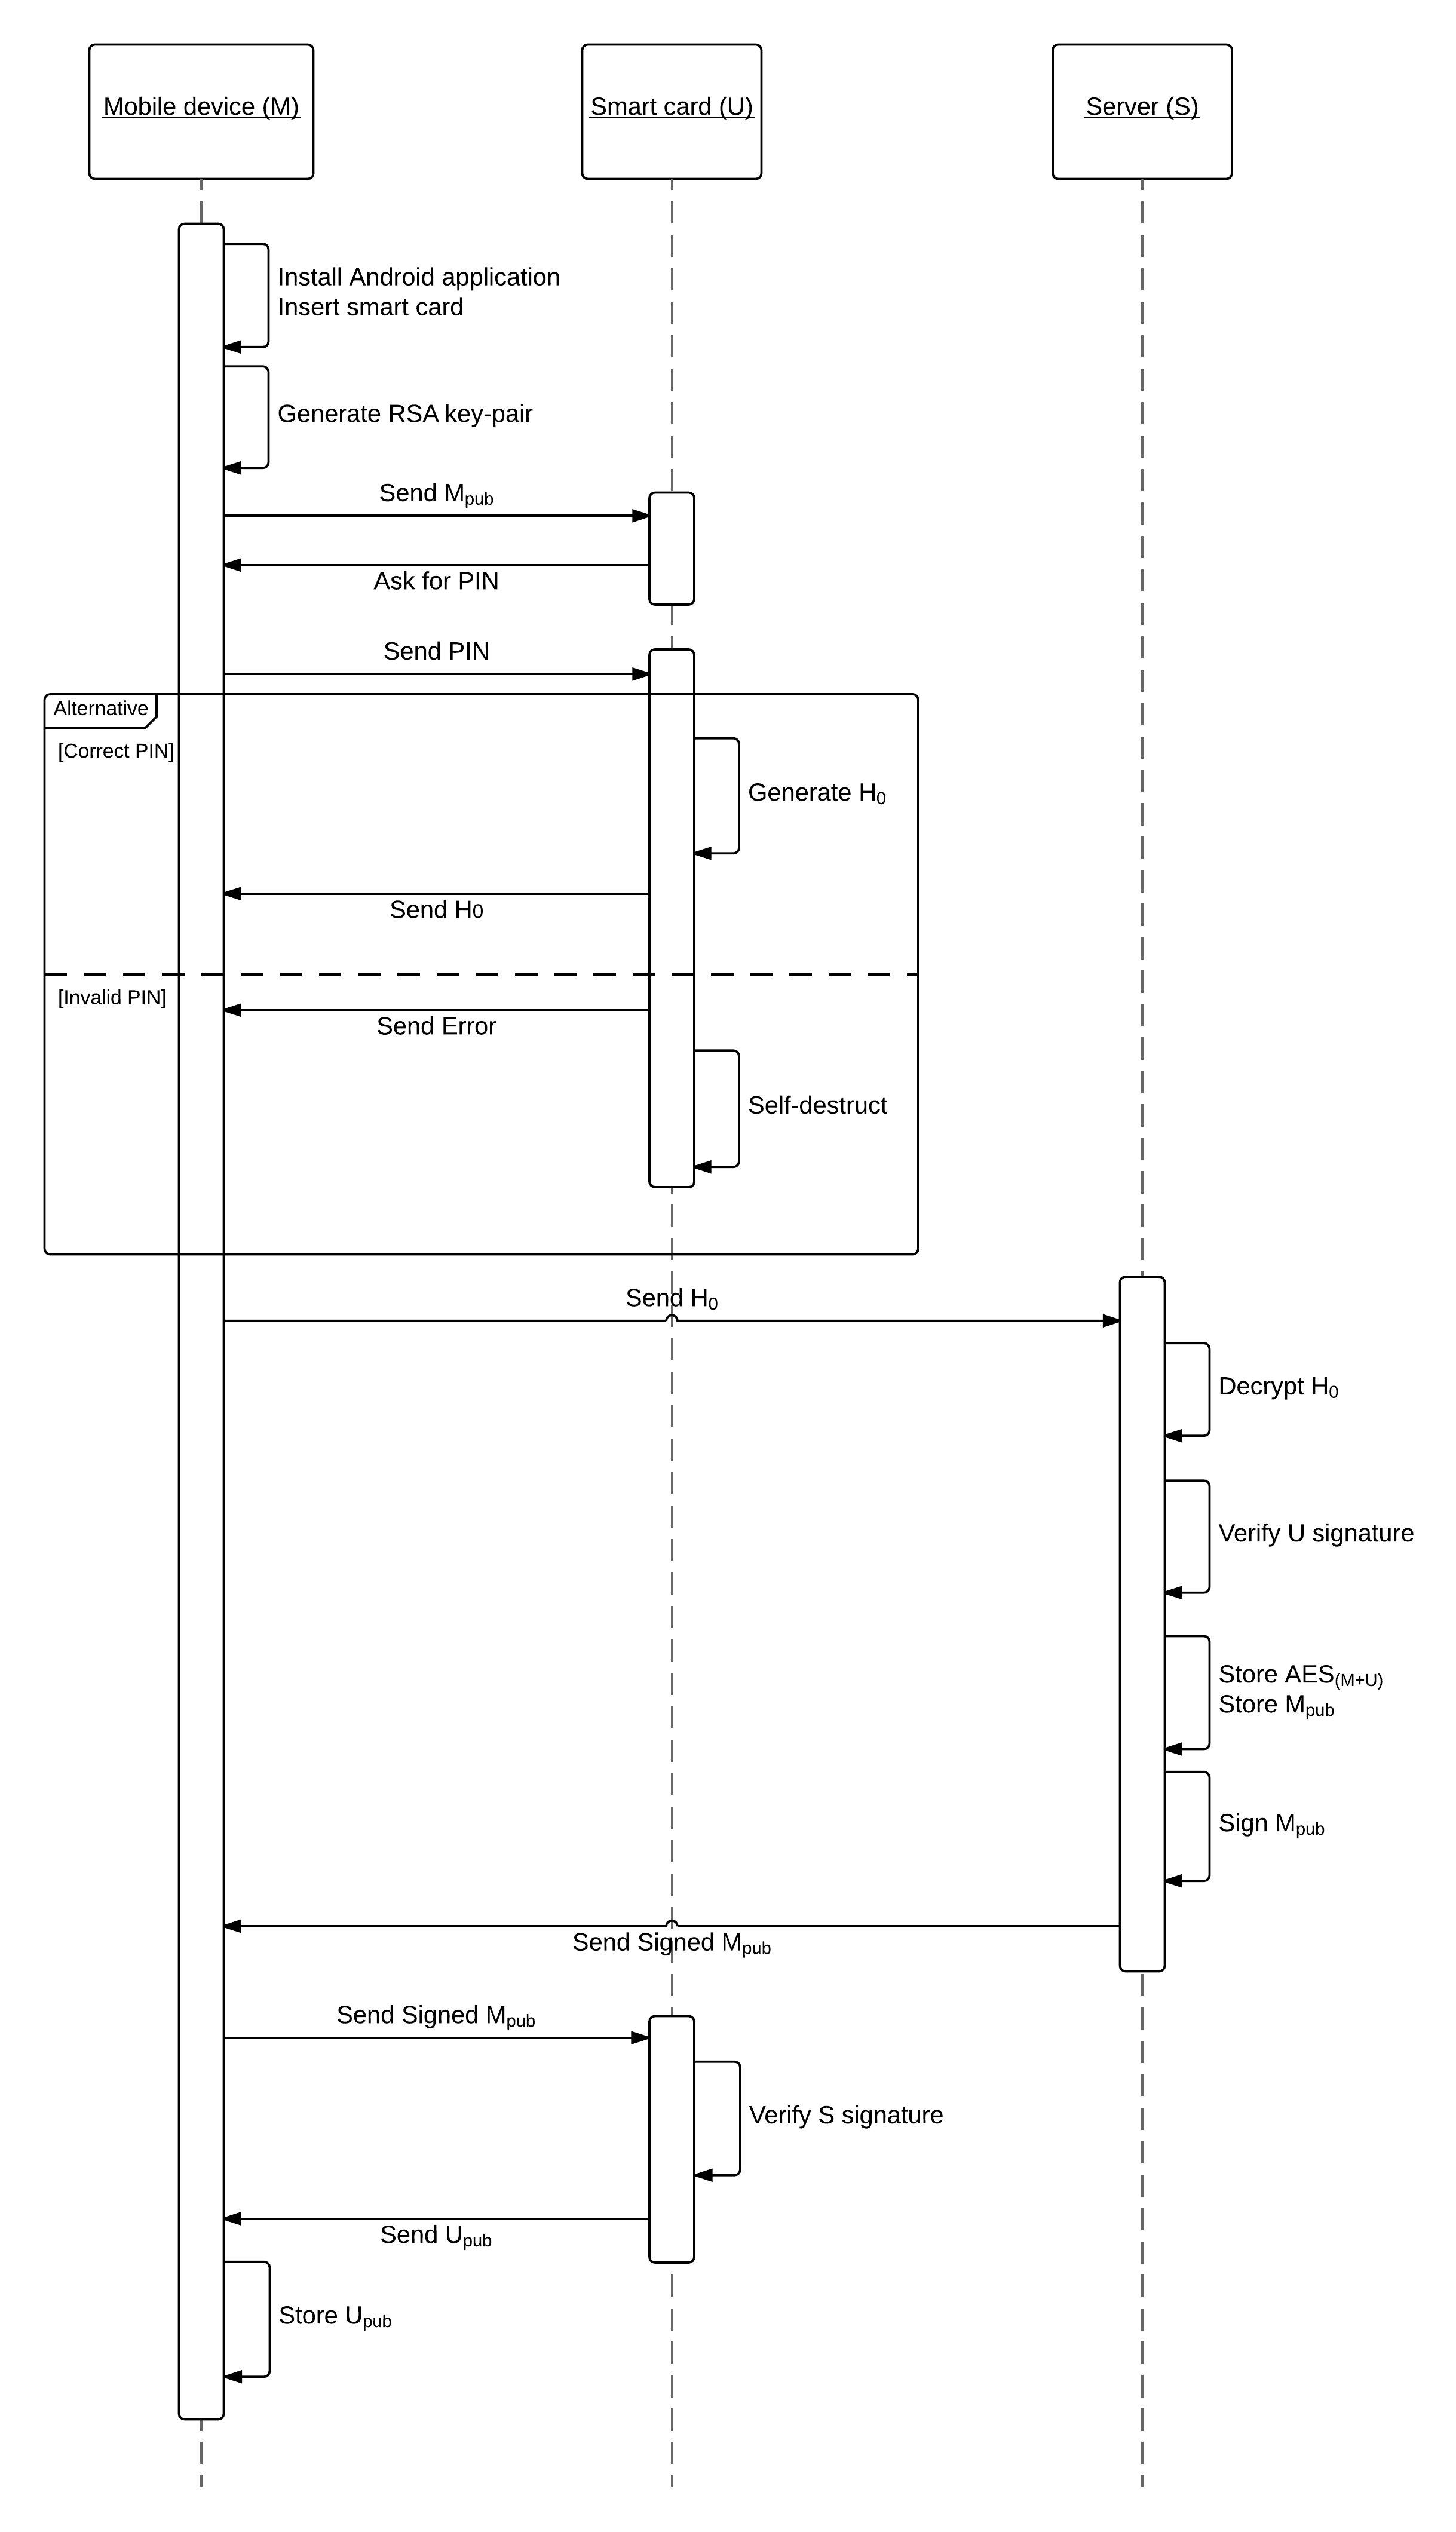
\includegraphics[height=0.93\textheight]{images/SQD_handshake.png}
\end{figure}
\clearpage
The end result of the transactions is that the smart card and mobile device have shared their public keys through the trusted third party and can thus communicate securely. The server will also have a record of the transactions and the parties. If we chose to do so we can also save a backup of the first symmetric key on the server.

Potentially we could add more steps to the process to further heighten the security. In step 7 we could add that a user may need to answer a challenge such as provide a one time password (OTP). This would add more overhead and require more resources administrating.

A direct consequence of a successful binding is that the smart card is now locked to the mobile device. Inserting the smart card into a different device will simply not work due to the fact that the smart card has the public key of the original device and they have already agreed upon a symmetric key. To further enhance this trait, we require the mobile device to identify itself if sensitive services are requested. This can be done by sending a challenge from the smart card to the mobile device which requires the private key of the original bound device to solve (e.g. challenge is encrypted with M\textsubscript{pub}). In addition since the smart card is able to securely communicate with the authority the smart card can lock itself up and require a signed package from the authority. This package could contain information regarding deletion of keys, force a new binding, etc. We discuss this possibility further in section \ref{sec:policies}.

\subsection{Protocol analysis}
In this section we will justify and evaluate the parts of the solution that have security implications. Steps that are present for the solution to function, but with no security implications, will be skipped.

\paragraph{1. Install the (correct) Android application the on mobile device (M) andinsert smart card (U).}\mbox{}\\
Installing the correct application is a vital part of the protocol. If the wrong Android application is installed the binding process will not complete and the user is not able to use the services we provide. As mentioned earlier we can use Google Play as our distribution platform which will minimize the risks involved.

\paragraph{2. M generates RSA key-pair and stores it securely on the device}\mbox{}\\
For the smart card to bind itself to a mobile device we need a unique identifier or key that no other device is able to replicate or spoof. An RSA key-pair provides this functionality as the mobile can use the private key to sign data and the smart card can encrypt data with the mobile device public key. Unless another mobile device is able to extract the private key we are in the clear security wise. More on this and other solutions in section \ref{sec:mobileDeviceKeys}.

\paragraph{4. U asks for PIN/OTP}\mbox{}\\
We chose to add a PIN code step to the binding process to add another layer of security. The PIN code ensures that a person is verified by the employer to perform the binding process. Using PIN codes is not a guaranteed measure against someone unauthorized trying to carry out the binding process. The important steps to make sure the PIN code process is secure are:
\begin{itemize}
  \item The binding process should be carried out as soon as possible after obtaining the PIN code to avoid someone leaking or losing the PIN code.
  \item Add a limited number of tries for inputting the PIN code on the smart code to mitigate brute-force attacks.
  \item In connection to the previous point; the PIN code length should correspond to the number of tries.
\end{itemize}

\paragraph{5. M provides PIN/OTP}\mbox{}\\
At some point the user will need to supply the mobile device the PIN or OTP in order for the mobile device to send it to the smart card. Theoretically an attacker can have compromised the device and intercept the PIN/OTP to use it with another device. This scenario is unlikely as the attacker will also need to get the physical smart card before the binding process is completed. Potentially an attacker can perform a denial of service attack in this step and never let the binding process complete. In section \ref{sec:attackVectors} we discuss the possibility to use Google SafetyNet to detect malware on the device.

\paragraph{6. U generates the verification package.}\mbox{}\\
The smart card is a secure environment and should be in charge of generating the verification package. We include the AES key for safekeeping on the server incase the user lose the smart card. We sign the package using the private key of the smart card and the server can verify that it is a legit smart card since the server has the public key. This step is necessary as anyone would be able to send a verification package to the server as the server public key is public. Lastly the smart card encrypts the verification package using the server's public key. The end product, the verification package, is secure in the sense that only the server can read the data and the server can authenticate the sender using the signature.

\paragraph{7. M connects to the server (S) and sends the verification package to S.}\mbox{}\\
The verification package is encrypted with the server's public key. The direct result is that even if the package is lost or leaked no third party would be able to read the content. We will use TLS for the connection regardless as it may be necessary to add additional functionality such as username-password login to verify the user. To establish a TLS connection one would access to the server certificate either via a third party certificate provider or via a pre-installed certificate. TLS will also serve as a counter to replay-attacks and man-in-the-middle attacks.

\paragraph{9. The server signs the public key of M.}\mbox{}\\
If the signature of the smart card is in order we can proceed with generating the response package. The server signs the public key of the mobile device. This is done because of the need to confirm that the verification package was indeed sent to the server. By letting the server sign it we ensure that the public key that is sent back to the smart card is in fact the public key that was in the verification package.

\paragraph{11. U verifies that M\textsubscript{pub} was signed by S and if successful U sends U\textsubscript{pub} to M.}\mbox{}\\
Even though public keys usually are publicly known we choose to keep the public key of the smart card semi-public or on a ``need to know basis''. Using this technique F not inherently make the solution secure, but it does add another hurdle a potential attack will need to overcome. In theory, the more steps an attacker will need to do; the higher the chance for detecting him. By rotating the keys the effectiveness of this measure increases substantially.


\subsection{Cryptography evaluation}
This solution relies heavily on correct use of protocols such as TLS (communication), cryptography such as RSA and AES, and correct key generation. Section \ref{sec:publicKeyCrypto} and section \ref{sec:symmetricCrypto} describes RSA and AES and why they are secure. Assuming we use them correctly we can conclude that this part of our solution is secure.
\iffalse %COMMENT
One of the most common public-key cryptosystems (refer to section \ref{sec:publicKeyCrypto}) is RSA, which is widely used for secure communication. RSA builds on the principle of factorization of the product of two prime numbers, or rather the difficulty of factorize the product. It is not impossible to factorize the product of two prime numbers and there was a challenge by the RSA Laboratories where one could win prizes for factorized RSA-keys \cite{rsaChallenge}, but the most complex RSA that were cracked was 768-bit. Proving that RSA is secure is out of the time scope for this thesis. Other source conclude that with long enough keys and correct protocol implementation, the math behind RSA can be considered secure \cite[~p. 194]{cryptoMath}. Information on the inner workings of RSA can be found in the book ``Understanding Cryptography'' by Christof Paar and Jan Pelzl, chapter 7 ``The RSA Cryptosystem'' \cite{cryptoMath}.

We are not directly utilizing the symmetric-key cryptography system AES, but it is an important aspect of the solution none the less. AES does not rely on number factorization, but rather substitution and permutation using a key. It can be seen as hashing data and being able to reverse the hashing using the same key. There are currently no known analytic attacks against AES which are less complex than brute-force attacks and we can thus conclude that using long keys are to be considered secure \cite[~p. 116-117]{cryptoMath}.

\fi %UNCOMMENT

In the solution we mitigate man-in-the-middle attacks using TLS for secure communication. TLS can utilize both RSA and AES and if we use strong keys we deem it secure (assuming TLS 1.2) from a mathematical perspective. If TLS is implemented correctly and does not allow for common attacks (Heartbleed, DROWN \cite{drown}, etc.) it is classified as ``probably secure'' or ``secure until proven otherwise''.

Correct key generation is discussed in section \ref{sec:mobileDeviceKeys} and the conclusion is that it is possible to securely generate keys. All cryptographic parts of the solution is considered secure if done correctly and we can thus conclude that the cryptography included in the solution is secure.
%TODO


\subsection{Potential attack vectors}
\label{sec:attackVectors}
%This solution relies heavily on correct use of protocols such as TLS (communication) and correct key generation. We assume that all cryptographic functions we use are used correctly and all keys are of such lenghts that they are cryptographically strong. Now that we have established that requirement we can look at the different attack vectors.

\paragraph{Rogue technical party}\mbox{}\\
The three technical parties involved are the server, the mobile device and the smart card. As discussed previously ``the authority'' issues the smart cards and administrates the server. Since the public keys and certificates are exchanged before the smart card is distributed the server is able to detect if there are a rogue/fake smart card trying to bind to a mobile device. If the mobile device tries to connect to the wrong server (man-in-the-middle attack, wrong URL, etc.) and the server tries to pose as a legit server, it will not be able to complete the binding process due to needing the matching private key for the public server key on the smart card.

Thus the only attack vector on technical parties is where the mobile device is rogue. By rogue in the context of the mobile device we mean compromised as in rooted or malware/spyware. In our solution we have no way of knowing if the user is binding a rogue mobile device. The end result is that we have securely bound the mobile device and smart card, but the mobile device cannot be trusted.

To address this we need to do two things. First and foremost we need to educate the user on mobile security and how they should not install applications from untrusted sources etc. Secondly we can run tests on the mobile device to try and detect if the mobile device is rooted or has malware/spyware. This can prove to be hard as it is very difficult, if not impossible, to detect malware/spyware which operate with root access. Google has been working on a security framework, SafetyNet, which goal is to detect if a device has been tampered with or is infected \cite{googleSafetynet}. In order to decide if this is sufficient we would have to do more research on SafetyNet specifically.

\paragraph{Rogue user or administrator}\mbox{}\\
Potentially we can have a rogue user which deliberately installs malware/spyware on their mobile device to compromise our system. We will disregard this case as if we have a rogue user we have bigger problems than a compromised mobile device. It is also important to note that any information the mobile device receives the user is also likely to know regardless, and can thus release this information independently of the mobile device.

The bigger problem would be a rogue administrator. The administrator would have access to the initial setup of the smart cards and may extract the private key of the server. Even though this has more impact than a rogue user we are very limited on what we can to do protect against it. We can make it near impossible to extract private keys, logging and require more than one administrator, but it will still be possible to cause harm. Although the same principle applies here: if you have a rogue administrator you have bigger problems than smart card binding.


\subsection{Additions}
In step 9 and 10 of the proposed solution we can add a payload to the signed M\textsubscript{pub}. One of the uses for this payload may be to send information on how the smart card should handle communication, key generation, encryption \& decryption as well as administration. More on this in section \ref{sec:policies}.


\section{Mobile device keys}
\label{sec:mobileDeviceKeys}


\subsection{Problem description}
Even though one of the features of the smart card is to store and manage keys, we are still dependent on the mobile device being able to securely store at least one set of keys. This is directly tied to the binding process of the mobile device and the smart card which were discussed in section \ref{sec:bindingcardandphone}. The problem lies in the fact that we assume that the key pair generated by the mobile devices cannot be extracted and installed on another device and can only be used by our application. The question is: how we can be sure that this is the case? We have no way of proving that the keys are generated on the mobile device. And even if we were, are they stored securely? We can also envision that there might emerge other use cases at later stages which require keys on the mobile device.

\subsection{Goals}
Our primary goals for mobile device keys are:

\begin{itemize}
  \item Make sure that the device keys are actually on the device.
  \item Store keys securely, ensuring that they cannot be exported or used by other applications or devices.
\end{itemize}

\subsection{Key concepts}

\paragraph{Android Keystore system}\mbox{}\\
The Android Keystore system is a system that lets users and developers store and access cryptographic keys and certificates on the mobile device. The main goal of the system is to protect the keys against unauthorized use and extraction. This is done by defining which applications that should have access to the keys stored. E.g. application A generates and stores a key and defines that the key is available to application A and B. If application C tries to access the key the Android Keystore system blocks the action.

The applications do not have direct access to the keys. If an application wants to perform a cryptographic operation it feeds the data to the operating system which performs the cryptographic operation. If an application is compromised an attacker gains access to the keys via the application, but the attacker is not able to extract the keys as the keys are never present in the application.

In early iterations the keys were stored in a software-protected file meaning that only the Android Keystore had access to the data. This system had a flaw in which any users or applications with root access could access the Keystore file. The solution to this is using secure hardware such as ``Secure Element'' (more or less a smart card) and ``Trusted Execution Environment (TTE)'' \cite{TEE}. If hardware-backed storage is enabled (as seen in figure \ref{fig:hardwareBacked}), it is not possible to extract keys even if the operating system is compromised.

\begin{figure}[h!]
  \captionsetup{justification=centering,margin=1.5cm}
  \caption{Screenshot of Android settings showing hardware-backed storage ``enabled''.}
  \label{fig:hardwareBacked}
  \centering
    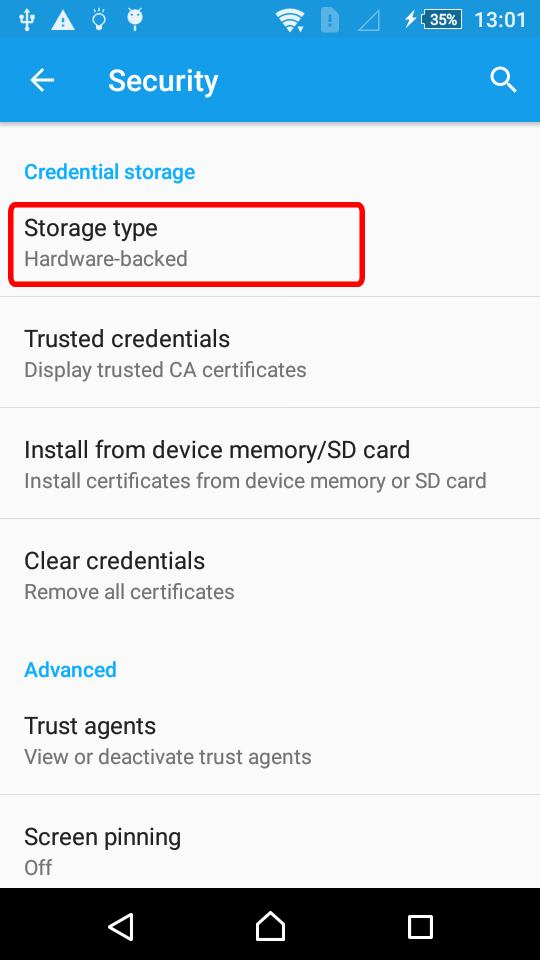
\includegraphics[width=0.45\textwidth]{images/hardwareBacked.png}
\end{figure}
An application can check if the mobile device uses secure hardware for key storage using the Android class \texttt{KeyInfo}. The \texttt{KeyInfo} class contains all available information about a key and a single call to the method \texttt{\allowbreak isInsideSecureHardware()} will determine the storage status. Listing \ref{lst:KeyInfo} provides a sample implementation of this functionality. \texttt{KeyInfo} was added in API 23 and requires Android version 6.0 or newer.


\begin{lstlisting}[caption=Obtaining storage status of keys using KeyInfo., label=lst:KeyInfo,escapechar=å]
public boolean checkStatus(PrivateKey key){
    KeyFactory factory = KeyFactory.getInstance(
        key.getAlgorithm(), "AndroidKeyStore");
    KeyInfo keyInfo;
    try {
         keyInfo = factory.getKeySpec(key, KeyInfo.class);
        å\colorbox{highlight}{return keyInfo.isInsideSecureHardware();}å
    } catch (InvalidKeySpecException e) {
        // Not an Android KeyStore key.
    }
    return false;
}
\end{lstlisting}

\subsection{Generate keys on mobile device}
To generate keys on the mobile device an application must initialize the classes \texttt{KeyGenerator} or \texttt{KeyPairGenerator}. \texttt{KeyGenerator} is used for generating symmetric secret keys and the most notable supported algorithms are AES(up to 256-bit), HmacSHA256 and HmacSHA512. As the name suggest \texttt{KeyPairGenerator} is used for generating key-pairs. Pre API level 23 it was possible to generate DSA key-pairs, but the support was removed in favour for more secure algorithms. The two main supported algorithms are RSA (up to 4096-bit) and Elliptic Curve algorithms (P-224, P-256, p-384 and P-521).

Generating long keys may put some strain on the mobile device and should either be done in an asynchronous thread or during a setup process on first time launch of the application. However this should not be a deciding factor of whether or not the mobile device should generate its own keys as it is a one time process. Listing \ref{lst:keygenAndroid} shows how an application can use \texttt{KeyPairGenerator} to generate a 4096-bit RSA key-pair.

\begin{lstlisting}[caption=Generating RSA key-pair on Android device using KeyPairGenerator, label=lst:keygenAndroid,escapechar=å]
public KeyPair generateKeyPair(){
    KeyPairGenerator kpg = KeyPairGenerator.getInstance("RSA");
    kpg.initialize(4096);
    return kpg.generateKeyPair();
}
\end{lstlisting}

\subsection{Generate keys on server}
\label{sec:generateKeysOnServer}
The Android Keystore system accepts \textit{PKCS\#12} archive files which it then stores on the mobile device. The PKCS\#12 file can contain certificates, keys and key pairs \cite{pkcs12}. After the archive file is manually installed on the device, applications that are authorized are free to use the keys via the Android Keystore system. The consequence of this is that we do not have to rely on the mobile device to generate the secure keys.

The most interesting characteristic of this solution is that a company or a similar entity can have a dedicated server generating these archive files. The server is able to run more security software than a mobile device and can be treated as a secure environment for key generation.

The PKCS\#12 archive file can be protected by a password and should definitely be protected by one to be even considered secure. This does add more overhead to the process of distributing the PKCS\#12 files.

The biggest obstacle when using server generated keys is distribution. You do not want to hand the PKCS\#12 file to the user on a USB stick along with a password on a notepad as you cannot be sure that the USB is destroyed or wiped properly along with the password. The solution to this is hosting the PKCS\#12 file on a website. The only way to access the PKCS\#12 file is through a portal which requires two-factor authentication (or similar) which limits user to only access the PKCS\#12 file they are supposed to reach. The file is then downloaded onto the mobile device and the users can install the file from their device memory (see figure \ref{fig:hardwareBacked}).

This solution does not remove the need for the users to know the password for the PKCS\#12 file and the file will still reside in the device memory. The only solution to this is to have strict security policies where the memory is wiped afterwards as well as removing the accessibility of the PKCS\#12 file on the server (from a users perspective).

One alternative when it comes to distributing the password for the PKCS\#12 file is using a password generated from a seed (salt) located on the smart card. By using this alternative, only user with access to the smart card is able to install the PKCS\#12 file on their mobile device. As an added security mechanism the smart card can lock or delete the seed/password afterwards and only be reset by an administrator. This would give us a certain degree of control over which devices that can have the keys installed.

\subsection{Evaluation and comparison}
In the problem statement we pointed out the binding process being dependent on the security of the keys generated and stored on the mobile device. We know that we are able to store the keys securely on the mobile device as long as hardware-backed storage is enabled and is being used. It is also possible to check if a key is stored on hardware in an Android application. In other words we have a solution to the storage issue: Use a mobile device which supports hardware-backed storage and validate it in the Android application using \texttt{KeyInfo}. The white paper ``Analysis of Secure Key Storage Solutions on Android'' by Tim Cooijmans, Joeri de Ruiter and Erik Poll discusses hardware-backed storage further \cite{KeyStorage}.

Security-wise the key generation on the mobile device and on a server is very similar. If the key generation on the mobile device is done correctly with properly generated secure initialization vectors the process is considered secure. The only realistic attack vector on key generation is that the mobile device is running a custom operating system which has it's own implementation of how key generation is done. To address this scenario it may be necessary to use Google's security framework, SafetyNet, as mentioned in section \ref{sec:attackVectors} when we discussed attack vectors on the binding process.

The biggest benefit of generating the mobile device keys on a remote and secure server is that we can strengthen the insecure elements of the binding process. In the proposed solution of the binding process (section \ref{sec:proposedSolution}) we have to trust that the mobile device is a device that is supposed to perform the binding process. For example if an attacker is able to get his hands on a smart card before it is bound to a mobile device, he may try to start the binding process with his own device. We counteract this with requiring PIN code and the possibility of adding user authentication with the server. If the mobile device keys are pre-generated by a server and installed by a user on the mobile device, we can use these keys to verify that the device is authenticated (as other devices does not have the keys). A consequence of this is that we may be able to simplify some of the steps in the binding process as we can trust the mobile device.

The drawbacks of pre-generating the keys, apart from more overhead, is the distribution process, which can introduce new attack vectors. In section \ref{sec:generateKeysOnServer} we discussed how we could use a web server to distribute the keys. What is also worth mentioning is that this solution requires a web server to be maintained and protected. Such a system also places a lot of trust in the user's hands as he is responsible for deleting the PKCS\#12 file as well as not disclosing the password.

An other distribution solution is to have a trusted administrator install the keys on the mobile device. For some organizations this could be cumbersome as now all users will need to visit the ``headquarters''. This is a direct hindrance to the ``Bring your own device''-idea and can potentially introduce extra costs when it comes to human resourcing. Another key point to keep in mind is what should the protocol be if the organization wishes to update all keys? This would put a lot of stress on the distribution department.

However, we assume already that there is a trusted server involved in the binding process, so the PKCS\#12 file could simply be distributed together with the response package described in section \ref{sec:proposedSolution}. This does imply that we have solved the distribution of the server certificate issue which the PKCS\#12 can solve as it can contain the server certificate.

There is no definitive ``best solution'' to the key generation problem. It all boils down to the question: ``Can you afford the infrastructure needed for server generated keys?'' If the answer to that question is yes then there is a lot to gain by using server generated keys as we have discussed above. Opting for the cheaper solution, generate keys on mobile device, does not equal an non-secure solution, but we do sacrifice some control of the process.

\section{Security policy enforcement}
\label{sec:policies}

\subsection{Definition}
A security policy defines what measures a system needs to follow in order for the system, organization, group, etc. to be secure. Security policies are not necessarily a technological restriction/rule and can exist as a socially enforced rule. Examples of security policies are:
\begin{itemize}
  \item All employees needs to have a background check.
  \item All company doors will be locked after 4 pm.
  \item Password must be changed once a month.
  \item Sensitive data must be encrypted with AES-256.
\end{itemize}

\subsection{Problem description}
Enforcing security policies via a mobile device is not a new concept and there exist multiple third party solutions for enforcing them. One example is Microsoft Exchange ActiveSync which enforces policies such as minimum password length, disable camera and application blocking \cite{exchangePolicies, msExchangeCookBook}. ActiveSync utilizes the fact that a user must connect through Microsoft Exchange Server in order to access company resources and verifies if the mobile device has enforced the policies through the established connection \cite{exchangePoliciesTech}.

The problem in these types of solutions lies in the fact that you cannot trust the mobile device to actually enforce the policies. How does the server know if the mobile device is telling the truth about policy enforcement? What if the mobile device says it requires the user to enter a password, but does not enforce it?

\subsection{Goals}
By using smart cards in the context of policy enforcement we wish to achieve the following:
\begin{itemize}
  \item Policies are enforced.
  \item Not possible to spoof policy enforcement by the mobile device.
  \item Policies cannot be tampered with.
\end{itemize}
Optionally we want to achieve the following:
\begin{itemize}
  \item Policies can be updated.
\end{itemize}

\subsection{Shift responsibility to a trusted party}
One way of making sure that policies are enforced is to give the responsibility of the action to a trusted party. Imagine that company A have a policy which requires their employees to update their password on their personal computers once a month. If the user profiles only exists locally on the computers, company A has no way of checking if the users update their passwords and run the risk of the users saying they have updated the password without doing so. To address this issue, the user profiles are moved to company A's server and the personal computers now do a lookup for the user profiles on the server. In this case, A has control over the user profiles and can check if the passwords are updated.

The limiting factor to a solution like this is that the trusted party might not be able to perform the job. A trusted server might not be able to enforce locking doors after 4pm just as a smart card is not able to perform all jobs we want it to do. A big part of the job is to identify which part of a security policy action we can move to the smart card to enforce the security policy.

\subsection{Proposed solution}
\label{sec:policySolution}

\paragraph{Relevant policies for a smart card}\mbox{}\\
The smart card is limited in what kind of policies it is able to enforce. It cannot enforce policies regarding forcing the mobile device into doing things only the mobile device controls. The smart card can provide vital data needed for performing an action, but it is up to the mobile device to actually perform the action. This effectively rules out policies such as, ``The mobile device must encrypt all files stored locally.'', since we can only provide the keys to do so, but the mobile device has to perform the action. We have to assume that the mobile device, more specifically the running application, wants to perform the action.

The core abilities of a smart card are: generate keys, store keys, encrypt and decrypt small amounts of data, sign data and store variables. We can make the application rely on the keys generated and stored in the smart card and as a result we have full control over the keys. The smart card can as a result enforce policies such as key rotation, key size and key availability (unlock key with PIN). A more general use case is to have the smart card refuse to provide services or information to the application if certain conditions are not met or if one suspect that the device might be compromised.

\paragraph{Installing policies}\mbox{}\\
One disadvantage of using smart cards is that once an applet has been installed it is a static application. It is not possible to add new code to a running applet. What we can do is to program all policies we may wish to utilize and disable them. With this technique we can dynamically turn on and off policies, given that we are able to communicate with the card. The first premise is to install all possible security policies we may need on the smart card before shipping the smart card to the user. The second premise is to translate all policies to a set of parameters which can be combined logically to form rules. If both premises are met we are able to manipulate the parameters and effectively changing the rules.

\paragraph{Enable and update policies}\mbox{}\\
To enable policies or set parameters for the policies we require a protocol to exchange information with the smart card from a server. One of challenges we have is ``How do we ensure that the mobile device relays policy updates to the smart card?''. One solution is to have the smart card lock itself and require a verification package from a trusted server after a number of operations. It is important to note that the smart card have no concept of time and therefore the smart card cannot use time to control lock cycles. A way to ensure that the server is the only party that can provide the verification package, is to utilize keys that are already on the smart card. For example the public key of the server or the symmetric key exchanged a the beginning of the binding protocol. Refer to figure \ref{fig:OH} and figure \ref{fig:NH} for challenge and challenge response.
%is to send a challenge from the smart card which only the server knows the answer to (shared key/secret).

\begin{figure}[h!]
  \captionsetup{justification=centering,margin=1.5cm}
  \caption{Smart card policy challenge.}
  \label{fig:OH}
  \centering
    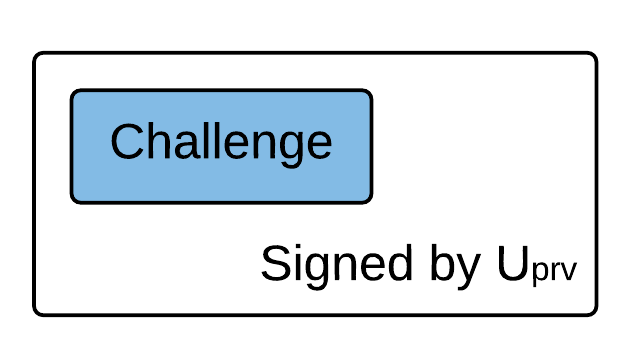
\includegraphics[width=0.65\textwidth]{images/challenge.png}
\end{figure}

\begin{figure}[h!]
  \captionsetup{justification=centering,margin=1.5cm}
  \caption{Smart card policy challenge response.}
  \label{fig:NH}
  \centering
    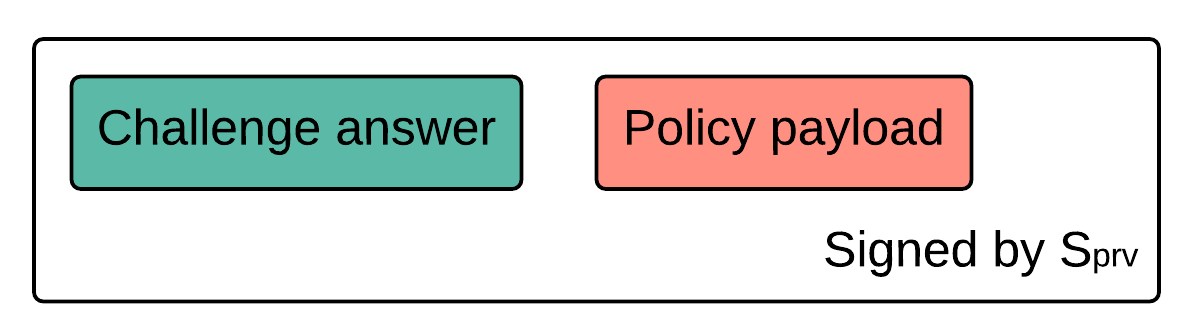
\includegraphics[width=0.75\textwidth]{images/challenge_response.png}
\end{figure}

\newpage

\paragraph{Challenge transaction}\mbox{}\\

U - Users smart card \\
M - Mobile device \\
S - Server, representation of authority \\
OH - Original hash \\
NH - New hash \\
\{Entity\}\textsubscript{prv} - Private key of an entity (U, M, S)\\

First we assume the binding of card and phone from section \ref{sec:bindingcardandphone} was successful. Secondly we assume that the server and smart card has a shared secret: a securely generated 256-bit AES key.

\begin{enumerate}
    \item U generates a challenge which is a long random hash (OH).
    \item U signs OH with U\textsubscript{prv}.
    \item U sends the signed OH package to S via the mobile device.
    \item S computes new hash (NH) using the AES key S and U agreed upon.
    \item S signs NH and the policy update.
    \item S sends the signed NH package (with policy update) to U via the mobile device.
    \item U computes the new hash and compares it to the NH it received.
    \item U applies policy updates.
\end{enumerate}

\begin{figure}[h!]
  \captionsetup{justification=centering,margin=1.5cm}
  \caption{Sequence diagram for smart card policy exchange.}
  \label{fig:SQD_policy}
  \centering
    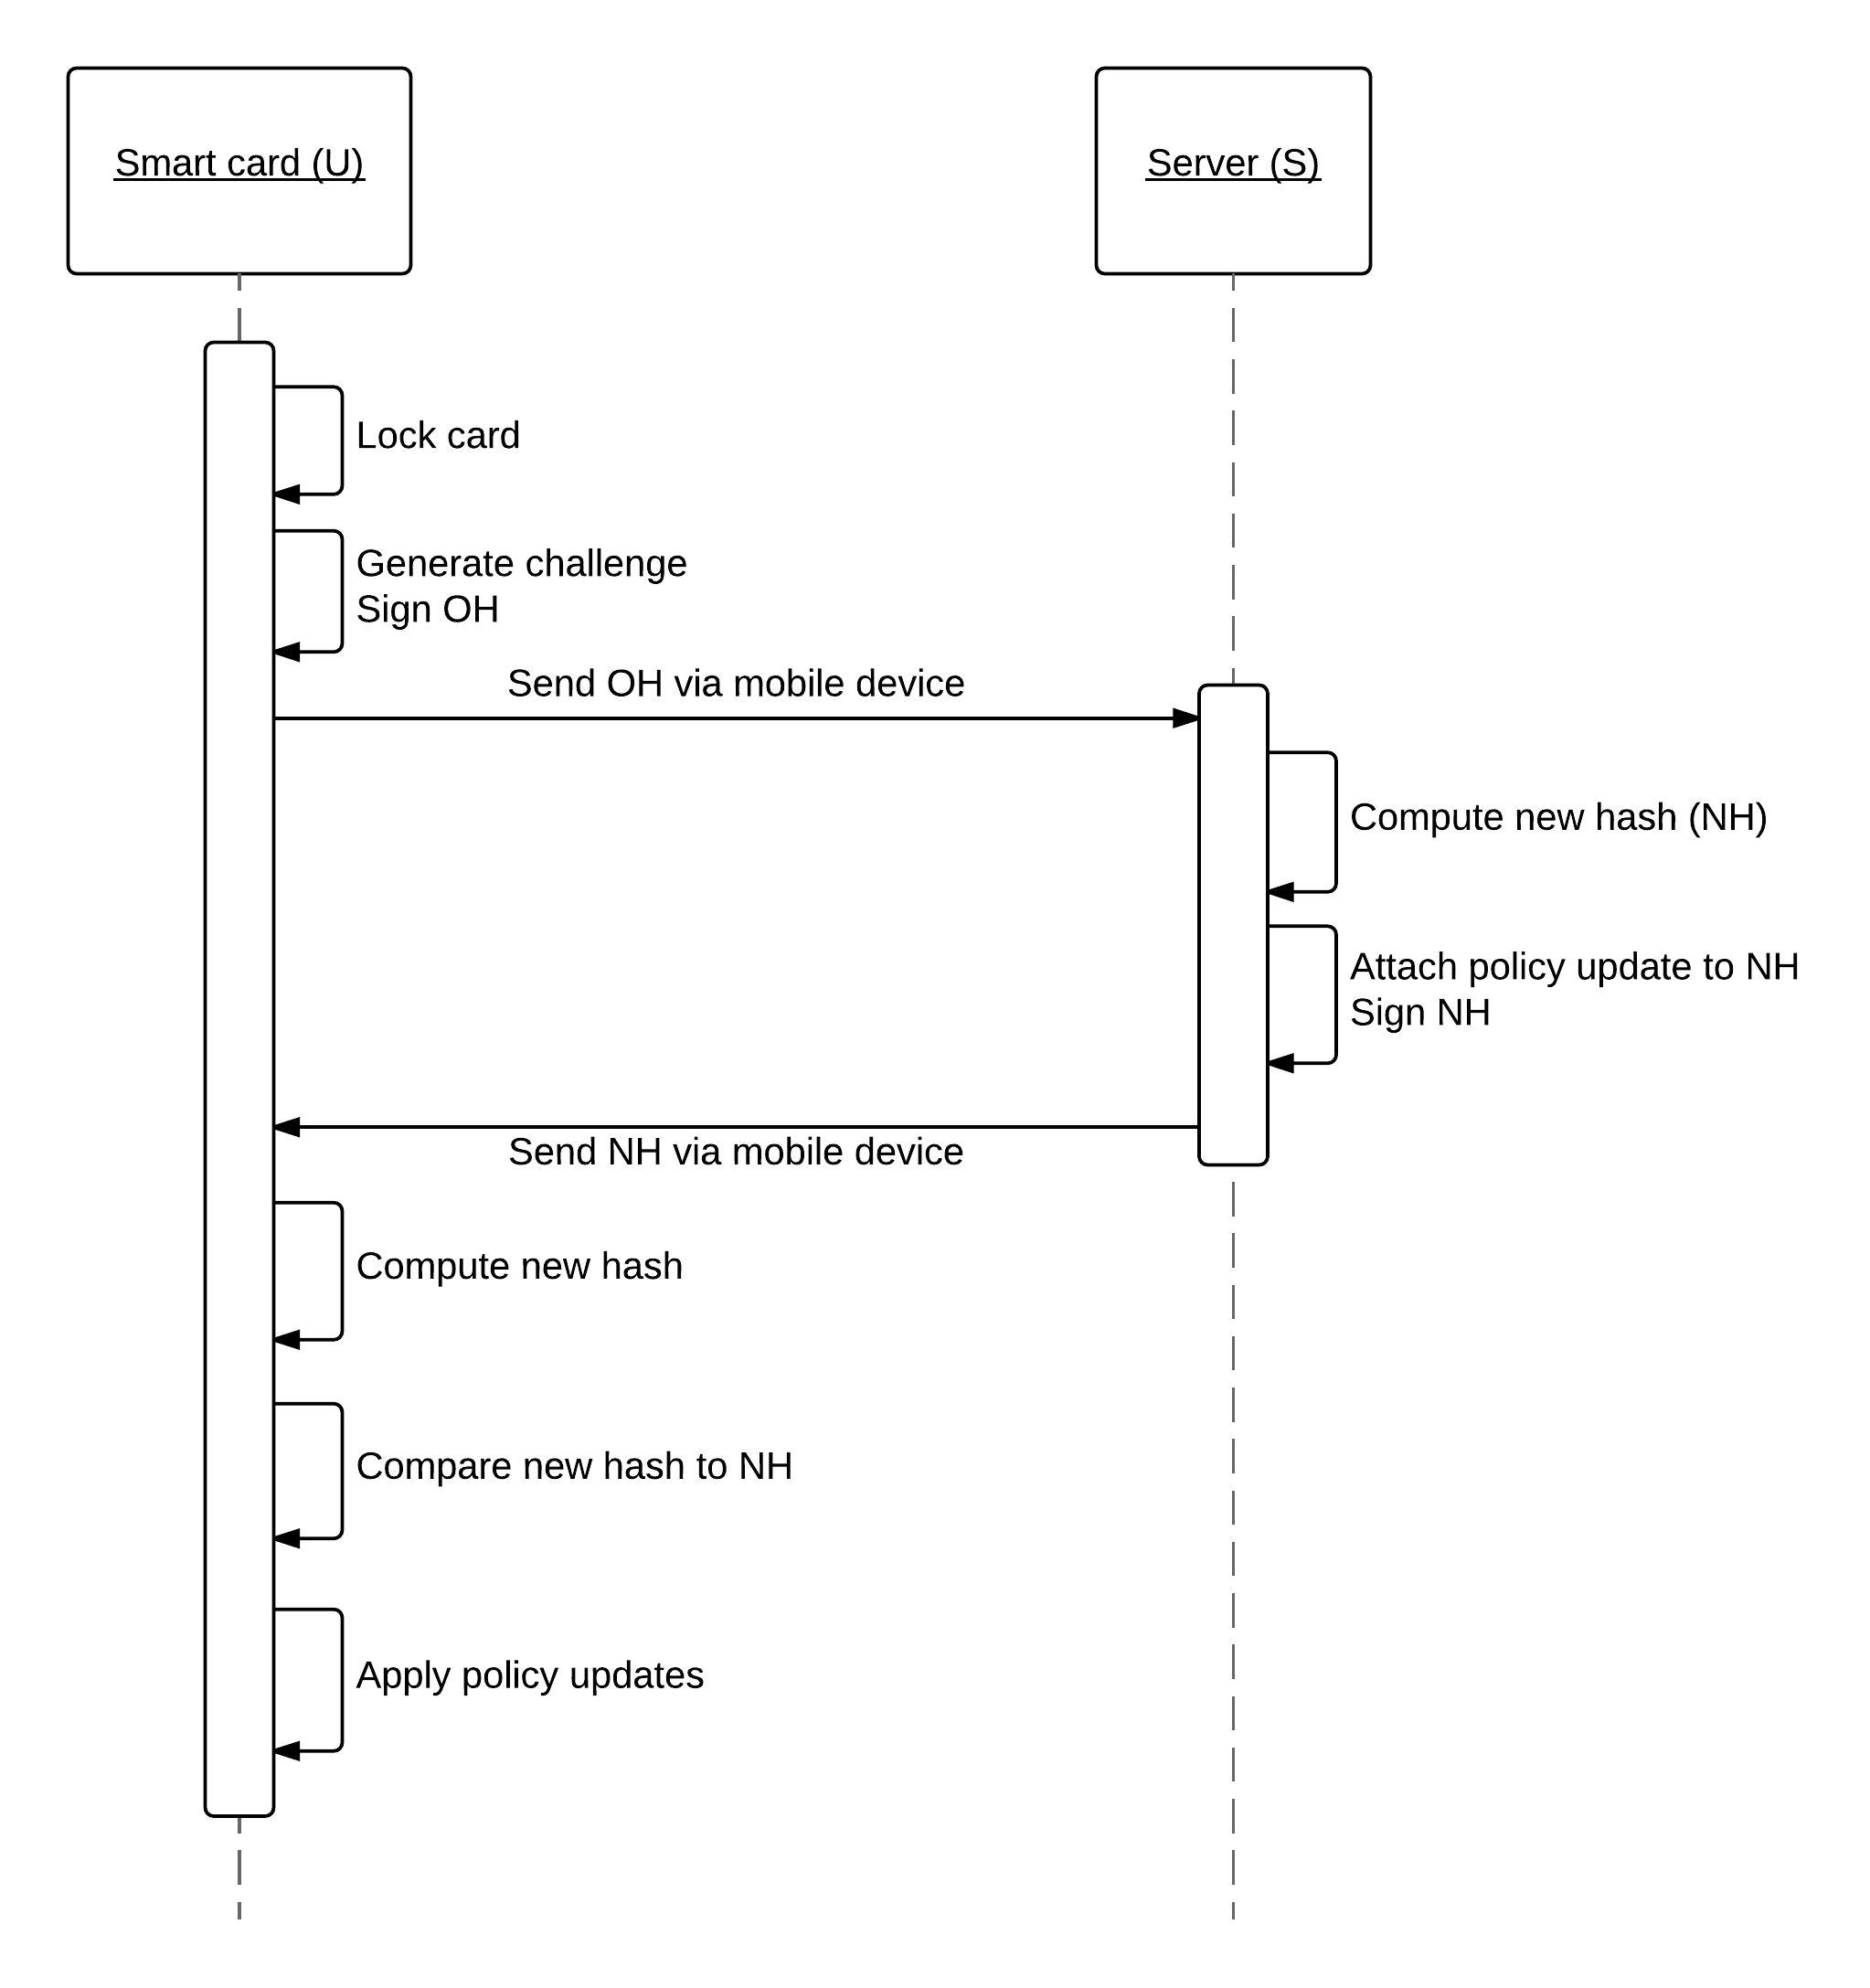
\includegraphics[width=0.95\textwidth]{images/SQD_Policy_Exchange.png}
\end{figure}

\newpage
%The "challenge" consists of a long random hash which is then signed by the smart card and sent to the server via the mobile device (see figure). The server computes the new hash using the AES key the smart card and server agreed upon. The new hash and any policy update is signed by the server and sent to the smart card.

\paragraph{Policy format}\mbox{}\\
When designing the format of the policy package there are two things to keep in mind. It should be human-readable for easy modification and not deviate too far from a machine-readable format as the smart card will need to interpret it. Another requirement to take into consideration is that data being sent to the smart card, must be converted to hex.

We can utilize JSON to make human-readable policies and as an added bonus JSON is readable for most programming languages. Listing \ref{lst:jsonPolicies} shows how this can be structured.
\begin{lstlisting}[language=json,firstnumber=1,caption=Human-readable policies in JSON., label=lst:jsonPolicies,]
{
  "policies": [
    {
      "id": "19",
      "description": "PIN attempts",
      "enabled": "true",
      "attempts": "3"
    },
    {
      "id": "21",
      "description": "Keylength (AES)",
      "enabled": "true",
      "keyLength": "256"
    }
  ]
}
\end{lstlisting}

Recall section \ref{sec:communicationstandard} where we described how a Command APDU must be structured. In the header we can use INS as a flag for ``policy update instruction'', for instance \texttt{09}. Next we have to look at what we technically want to achieve:
\begin{enumerate}
    \item Set boolean variable to true, depending on policy ID and ``enabled'' flag.
    \item Set other variable values.
\end{enumerate}
In the body we will use the payload data field to send information on the policy updates. The incoming data will be in byte format. Mapping bytes to variables could normally be solved using \texttt{HashMap} and map entries with \texttt{<byte, Object>}; the first parameter is the incoming byte command and second parameter being the variable we want to manipulate. \texttt{HashMap} is not a part of the Java Card API and we need to do our own hardcoded manual mapping. The result is a rigid structure for policies.

The individual policies data structure needs to be carefully crafted and specialized, but we should also focus on making it as dynamic as possible. This is best described using an example. To demonstrate how it can be done, we will use listing \ref{lst:jsonPolicies} as example data. The resulting APDU is figure \ref{fig:policyAPDU} and it clearly shows that we have to hardcode how many fields a policy will need.

\begin{figure}[h!]
  \captionsetup{justification=centering,margin=1.5cm}
  \caption{Example policy APDU with two policies}
  \label{fig:policyAPDU}
  \centering
    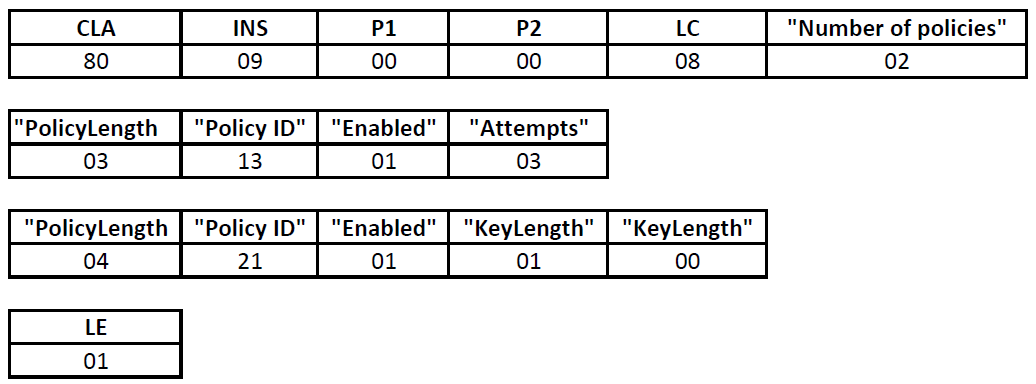
\includegraphics[width=0.95\textwidth]{images/policyAPDU.png}
\end{figure}

When designing the smart card code for interpreting the policy APDU we need a registry of some sort for keeping track of how much of the payload each policy uses. Listing \ref{lst:apduPolicy} uses figure \ref{fig:policyAPDU} as incoming APDU.

\begin{lstlisting}[caption=Pseudo code for interpreting policy APDU with Java Card., label=lst:apduPolicy,escapechar=å]
public class cardApplication extends Applet implements å\allowbreak åExtendedLength{
    ...

    //Policies
    final short offset = 5;
    short counter;

    //Policy 13
    boolean enabled13;
    short attempts;

    //Policy 21
    boolean enabled21;
    short keyLength;

    public void process(APDU apdu) {
    	...
        byte[] buff = apdu.getBuffer();

    	switch(buff[ISO7816.OFFSET_INS]){
            case 0x09:
                counter = 6;
                for(short i = 0; i < buff[offset]; i++){
                    if(buff[counter+1] == 13){
                        enabled13 = (buff[counter + 2] != 0);
                        attempts = buff[counter + 3];
                    }
                    else if(buff[counter+1] == 21){
                        enabled21 = (buff[counter + 2] != 0);
                        keyLength =
                            (short)((buff[counter+3]<<8)
                             | (buff[counter+4]))
                    }
                    counter += (1 + buff[counter]);

                }
                break;


            ...

    	}
    	Send(apdu);
    }

    private void send(APDU apdu) {
    	//Package outgoing buffer
    	//Send response APDU
    }
}
\end{lstlisting}

\subsection{Solution evaluation}
Section \ref{sec:policySolution} described how a smart card can enforce policies and how to manage policies. The solution is complex, intricate, requires a lot of overhead and is very rigid. Despite these drawbacks, using a smart card for policy enforcement could be well worth it. If an organization need a system where they are in full control and that is tamper proof, a smart card solution is viable option.

\subsection{Potential attack vectors}
\paragraph{Known-plaintext attack}\mbox{}\\
The challenge we use is simply two parties creating the same ciphertext from a hash and then comparing them. We then use digital signing to ensure that the challenge-response cannot be intercepted and spoofed. Since we do not encrypt the challenge-response in any way we have to vary of ``known-plaintext attacks'' \cite[~Ch. 2.3.2]{cryptoMath}. To protect against this type of attack the smart card and server must use keys that are long and algorithms that are difficult to brute-force. The final solution should use at least 256-bit long AES keys and as an added measure rotate keys.






%end

  % !TEX root = ../Article.tex
\chapter{Implementation}
In this chapter we will give an overview of the framework we have implemented along with implementation details. After reading this chapter the reader should have a good understanding of how the framework is built up and be able to utilize the framework in an Android application.

% !TEX root = ../../Article.tex
\section{Java Card applet}
The Java Card side of the complete framework includes functionality for performing basic data exchange with the Android application, basic cryptography and operations needed to implement the binding protocol. The goal of the smart card application was to create an autonomous and easy to extend platform for future tests. This resulted in an application split into three parts: initialization, data processing and finalization.

\paragraph{Initialization}\mbox{}\\
As described in section \ref{sec:javacard} all Java Card applications must implement the method \texttt{Install}. \texttt{Install} invokes the constructor of the smart card and this is where all variables that need initialization are initialized. For instance if the smart card application needs to generate keys or random numbers this is where it is done as the constructor will be invoked only once. All buffers that needs to be used should also be initialized here to avoid allocating memory every time the application is activated.

\paragraph{Data processing}\mbox{}\\
In the mandatory \texttt{Process} method (refer to section \ref{sec:javacard}) all data processing takes place. First a built in method in the Java Card API, \texttt{selectingApplet()}, is invoked. This method checks if the incoming APDU is a SELECT APDU and acts accordingly. If the incoming APDU is not a SELECT APDU the incoming APDU is copied to a new buffer for easier data manipulation. Next, we use a switch statement switching over the second byte, INS, to determine which instruction we want to perform. After processing the data and performing the work we want to do (sign data, encrypt, etc.) we copy our response to the outgoing buffer.

\paragraph{Finalization}\mbox{}\\
At the end of the \texttt{Process} invocation we invoke the \texttt{send} method which takes the data in the outgoing buffer, package it for sending and send it as a response APDU.

\paragraph{The result}\mbox{}\\
What we end up with is a test platform where we are only concerned with declaring variables, initializing variables and writing code for the specific test case. Listing \ref{lst:pseudoCard} shows pseudocode for the Java Card application with the extendable areas highlighted.


\begin{lstlisting}[caption=Pseudo code for javacard test application., label=lst:pseudoCard,escapechar=!]
public class cardApplication extends Applet implements ExtendedLength{

    !\colorbox{highlight}{//Variable declarations}!

    private cardApplication() {
    	!\colorbox{highlight}{//Variable initialization}!
    }

    public void process(APDU apdu) {
    	//Process incoming APDU
        if (selectingApplet()) {
			return;
		}
        buff = apdu.getBuffer();

    	switch(buff[ISO7816.OFFSET_INS]){
            case 0x00:
            case 0x01:
            !\colorbox{highlight}{...}!
            case 0xff:
            default:

    	}
    	Send(apdu);
    }

    private void send(APDU apdu) {
    	//Package outgoing buffer
    	//Send response APDU
    }
}
\end{lstlisting}

As seen in listing \ref{lst:pseudoCard} we allow for 256 cases/uses of the smart card, but if we include the use of P1 and P2 from section \ref{sec:communicationstandard} there are in theory 256\textsuperscript{3} = 16777216 possible cases. This does not include the pre-implemented methods which are explained in section \ref{sec:androidApp}. Their counterparts in the smart card application have the following byte values:

\begin{itemize}
    \item byte SEND\_U\_PUB\_MOD = (byte) 0x01;
    \item byte SEND\_U\_PUB\_EXP = (byte) 0x02;
    \item byte SIGN = (byte) 0x03;
    \item byte BINDING = (byte) 0x05;
    \item byte RSACRYPTO = (byte) 0x06;
    \item byte AESCRYPTO = (byte) 0x09;
\end{itemize}

\texttt{RSACRYPTO} and \texttt{AESCRYPTO} uses P1 to differentiates between encrypting and decrypting. \texttt{0x01} for encryption and \texttt{0x02} for decryption.
We will not go into detail on how the individual cases are built up as their functionality should be self-explanatory. Refer to Appendix A for Java Card code.

\subsection{Extending the Java Card application}
When adding more functionality to the Java Card application there are a few things to keep in mind. First of all one should follow the recipe shown in listing \ref{lst:pseudoCard} to minimize clutter and to follow the principles of Java Card programming. Secondly it is important to keep in mind that Java Card does not have standard garbage collection (refer to section \ref{sec:javacard}). A direct consequence is that any extension or extra functionality added to the smart card application may lead to ``Out of Memory'' errors.

Installation time of the smart card application may also be affected by extra functionality. Key generation on the smart card is a relatively expensive process, and one may find that it is not worth adding installation time to the whole application for one function. One approach is to split functionality in multiple applications. We will discuss this approach later in chapter \ref{ch:conclusion}, section \ref{sec:future}.

% !TEX root = ../../Article.tex
\section{Android Application}

\subsection{3rd party libraries}
Gemalto provides a java library, IDGo800, for communicating and utilizing built-in methods with their smart cards.

\begin{aquote}{Gemalto.com \cite{GemaltoIDGo800}}
``IDGo 800 for Mobiles is a cryptographic middleware that supports the Gemalto IDPrime cards and Secure Elements on Mobile platforms: Contact and contactless smart cards, MicroSD cards, UICC-SIM cards, embedded Secure Elements (eSE) and Trusted Execution Environment (TEE).''
\end{aquote}

The part of IDGo800 SDK we are interested in is very small and enables us to send custom APDUs to micro SD smart cards.

We will be using the ``android.nfc'' package in order to communicate with NFC smart cards. This package is included in the standard Android SDK which in turns means that all Android devices with a NFC reader and minimum API level 9 \cite{androidNFCminSDK} can use our library.

\subsection{Application}
\label{sec:androidApp}

In section \ref{sec:designAndroidGoals} we described the goals of the framework. The first goal we will describe the implementation of is ``extendable'' or in other words, being able to send custom APDUs. Explaining how this is implemented will give a better understanding of how the framework is built up and makes it easier to understand the pre-implemented methods.

We used the same approach on the Android application as on the smart card application; an autonomous and easy to extend plattform for tests. This resulted in a new library, ``smartcardlibrary'',  which sole purpose is to transmit APDUs as easily as possible along with some basic functionality.

\paragraph{Custom APDUs}\mbox{}\\
To send custom APDUs to a smart card,\texttt{CommunicationController} must be instantiated and the application must know the application identifier of the smart card application. Further the current activity must implement\\ \texttt{NfCSmartcardControllerInterface} or \texttt{MSDSmartcardControllerInterface} (depending on smart card type) in order to be notified when the transaction is complete. Before continuing one will need to call the methods \texttt{setupNFCController} or \texttt{setupmSDController} depending on the smart card. Listing \ref{lst:NFCLibraryExample} shows an example implementation on how an activity may utilize the library for sending custom commands to a NFC smart card.

\begin{lstlisting}[caption=Java code example showing how to send and receive commands to a NFC smart card., label=lst:NFCLibraryExample,escapechar=å]

public class PayloadActivity extends AppCompatActivity
    implements NFCSmartcardControllerInterface {
    CommunicationController cc = new CommunicationController();
    ...

    private void initNFCCommunication(){


        String AID = "0102030405060708090007";
        String hexMessage = "95404F3FB1";
        String INS = "06";
        String p1 = "00";
        String p2 = "00";
        cc.setupNFCController(this, this);
        cc.initNFCCommunication(AID, INS, p1, p2, hexMessage);
    }

    å@Overrideå
    public void nfcCallback(final String completionStatus){
        if(!completionStatus.equals("OK")){
            return;
        }
        StorageHandler stHandler =
            new StorageHandler(getApplicationContext());
        String response =
            stHandler.readFromFileAppDir(
                FilePaths.tempStorageFileName
            );
    }
}

\end{lstlisting}

In order for the library to perform an asyncronous transaction the library will temporary save the responses from the cards to a file only accessible by the running application. To retrive the data the current activity should use the included \texttt{StorageHandler} class as used in listing \ref{lst:NFCLibraryExample}. The library also provides the class, \texttt{Converter}, for converting between Strings, hex and byte arrays.

\paragraph{Pre-implemented methods}\mbox{}\\
Recall the areas we want to cover from the beginning of the chapter. The functionality we have implemented so far are:

\begin{itemize}
    \item Bind smart card to mobile device.
    \item Encrypt/decrypt data using RSA key on card.
    \item Encrypt/decrypt data using AES key on card.
    \item Get public key of the smart card.
    \item Sign data using the public key of the smart card.
\end{itemize}

To use these functionalities one would only need to create an Android \texttt{Activity}, invoke either \texttt{setupNFCController(...)} or \texttt{setupmSDController(...)} (depending on smart card), and utilize the desired methods. In figure \ref{fig:instantiateflow} we can see how \texttt{CommunicationController} is designed to be the abstraction layer between Android activities and smart cards.


\begin{figure}[h!]
  \caption{Abstraction layer between Android activities and smart cards.}
  \label{fig:instantiateflow}
  \centering
    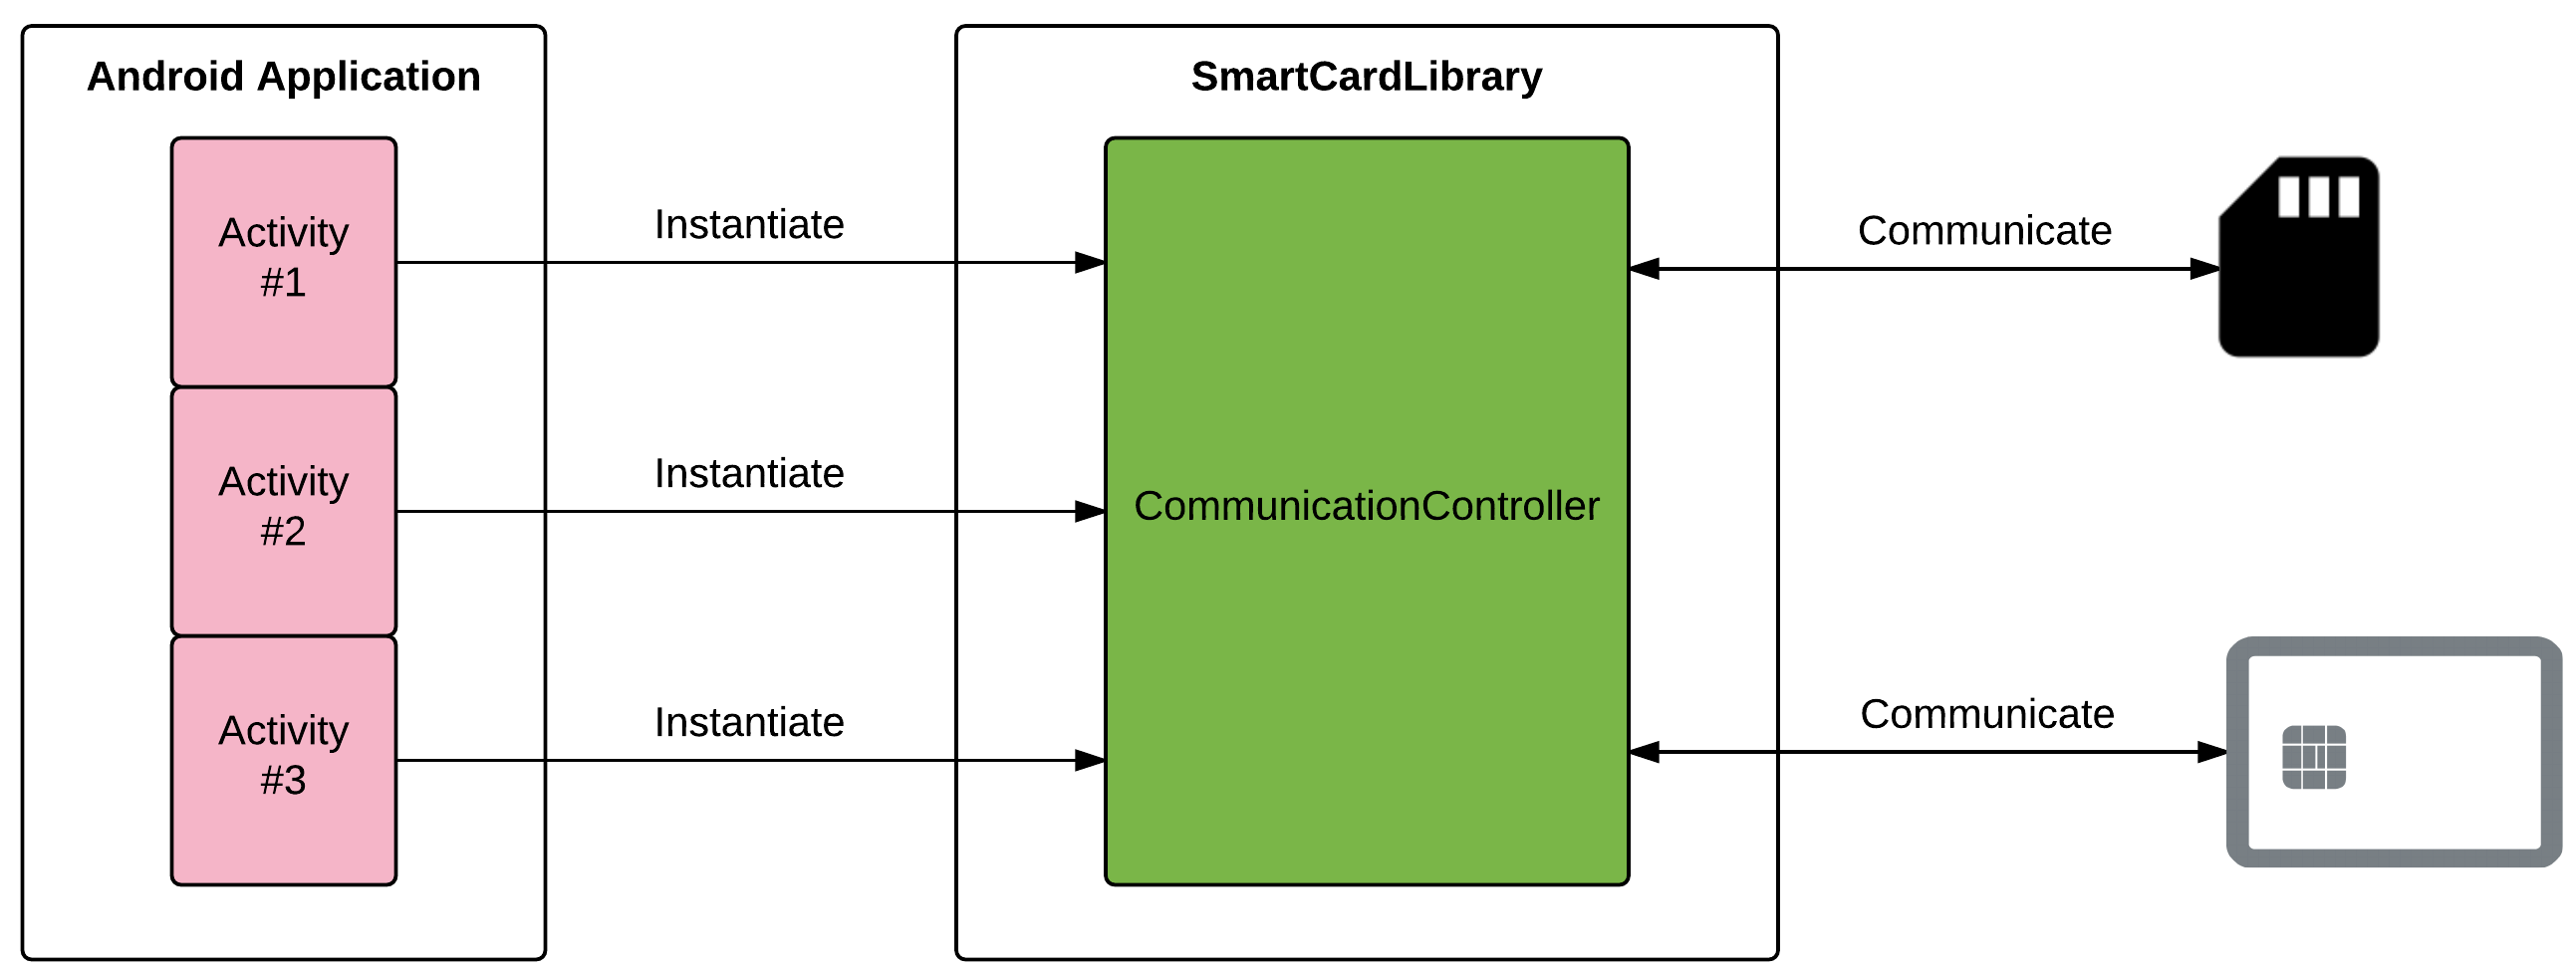
\includegraphics[width=0.95\textwidth]{images/Instantiate_flow.png}
\end{figure}

The methods available are:

\begin{itemize}
    \item public void disableNFC(...)
    \item public void signData(...)
    \item public void cryptoRSA(...)
    \item public void cryptoAES(...)
    \item public void getCardPubMod(...)
    \item public void getCardPubExp(...)
    \item public void bindingStepOne(...)
    \item public void bindingStepTwo(...)
    \item public void bindingStepThree(...)
\end{itemize}

The methods and their functionality should be self-explanatory except for the binding process. The binding process is designed in three steps. First step is to ask the smart card if it requires a PIN-code and how many attempts are left. Second step requires a PIN-code and if this is correct the smart card application will move on to step three. The last step is sending the public key of the mobile device and getting the verification package from section \ref{sec:proposedSolution}. More discussion on this matter in section \ref{sec:bindingcardandphone}.

Listing \ref{lst:NFCSigning} shows how an activity can use the \texttt{CommunicationController} to sign a simple message. The \texttt{signData(...)} method takes 3 parameters: CommunicationType, AID and the hex message to be signed. In the method \texttt{nfcCallback(...)} the developer are free to do whatever they want. Typically it is a good idea to check what the completeionStatus is before trying to fetch the response data. Refer appendix \ref{app:b} for all method signatures.

\begin{lstlisting}[caption=Java code example showing how to send sign a message using a NFC smart card., label=lst:NFCSigning,escapechar=å]

public class SigningActivity extends AppCompatActivity
    implements NFCSmartcardControllerInterface {
    CommunicationController cc = new CommunicationController();
    ...

    private void initNFCCommunication(){


        String AID = "0102030405060708090007";
        String message = "This message must be signed.";
        String hexMessage = Converter.StringToHex(message);
        cc.setupNFCController(this, this);
        cc.signData(CommunicationType.NFC, AID, hexMessage)
    }

    å@Overrideå
    public void nfcCallback(final String completionStatus){
        if(!completionStatus.equals("OK")){
            return;
        }
        StorageHandler stHandler = new StorageHandler(
          getApplicationContext()
          );
        String response = stHandler.readFromFileAppDir(
          FilePaths.tempStorageFileName
          );
    }
}

\end{lstlisting}


Figure \ref{fig:classdiagram_simple} provides a simplefied and technical overview of how the Android side of the library is built up. This diagram also shows which parameters are required for the methods available in \texttt{CommunicationController}. The complete class diagram for the Android library can be found in Appendix \ref{app:c}, figure \ref{fig:classdiagram_extended}.

\begin{figure}[h!]
  \caption{Simplefied class diagram for Android Library.}
  \label{fig:classdiagram_simple}
  \centering
    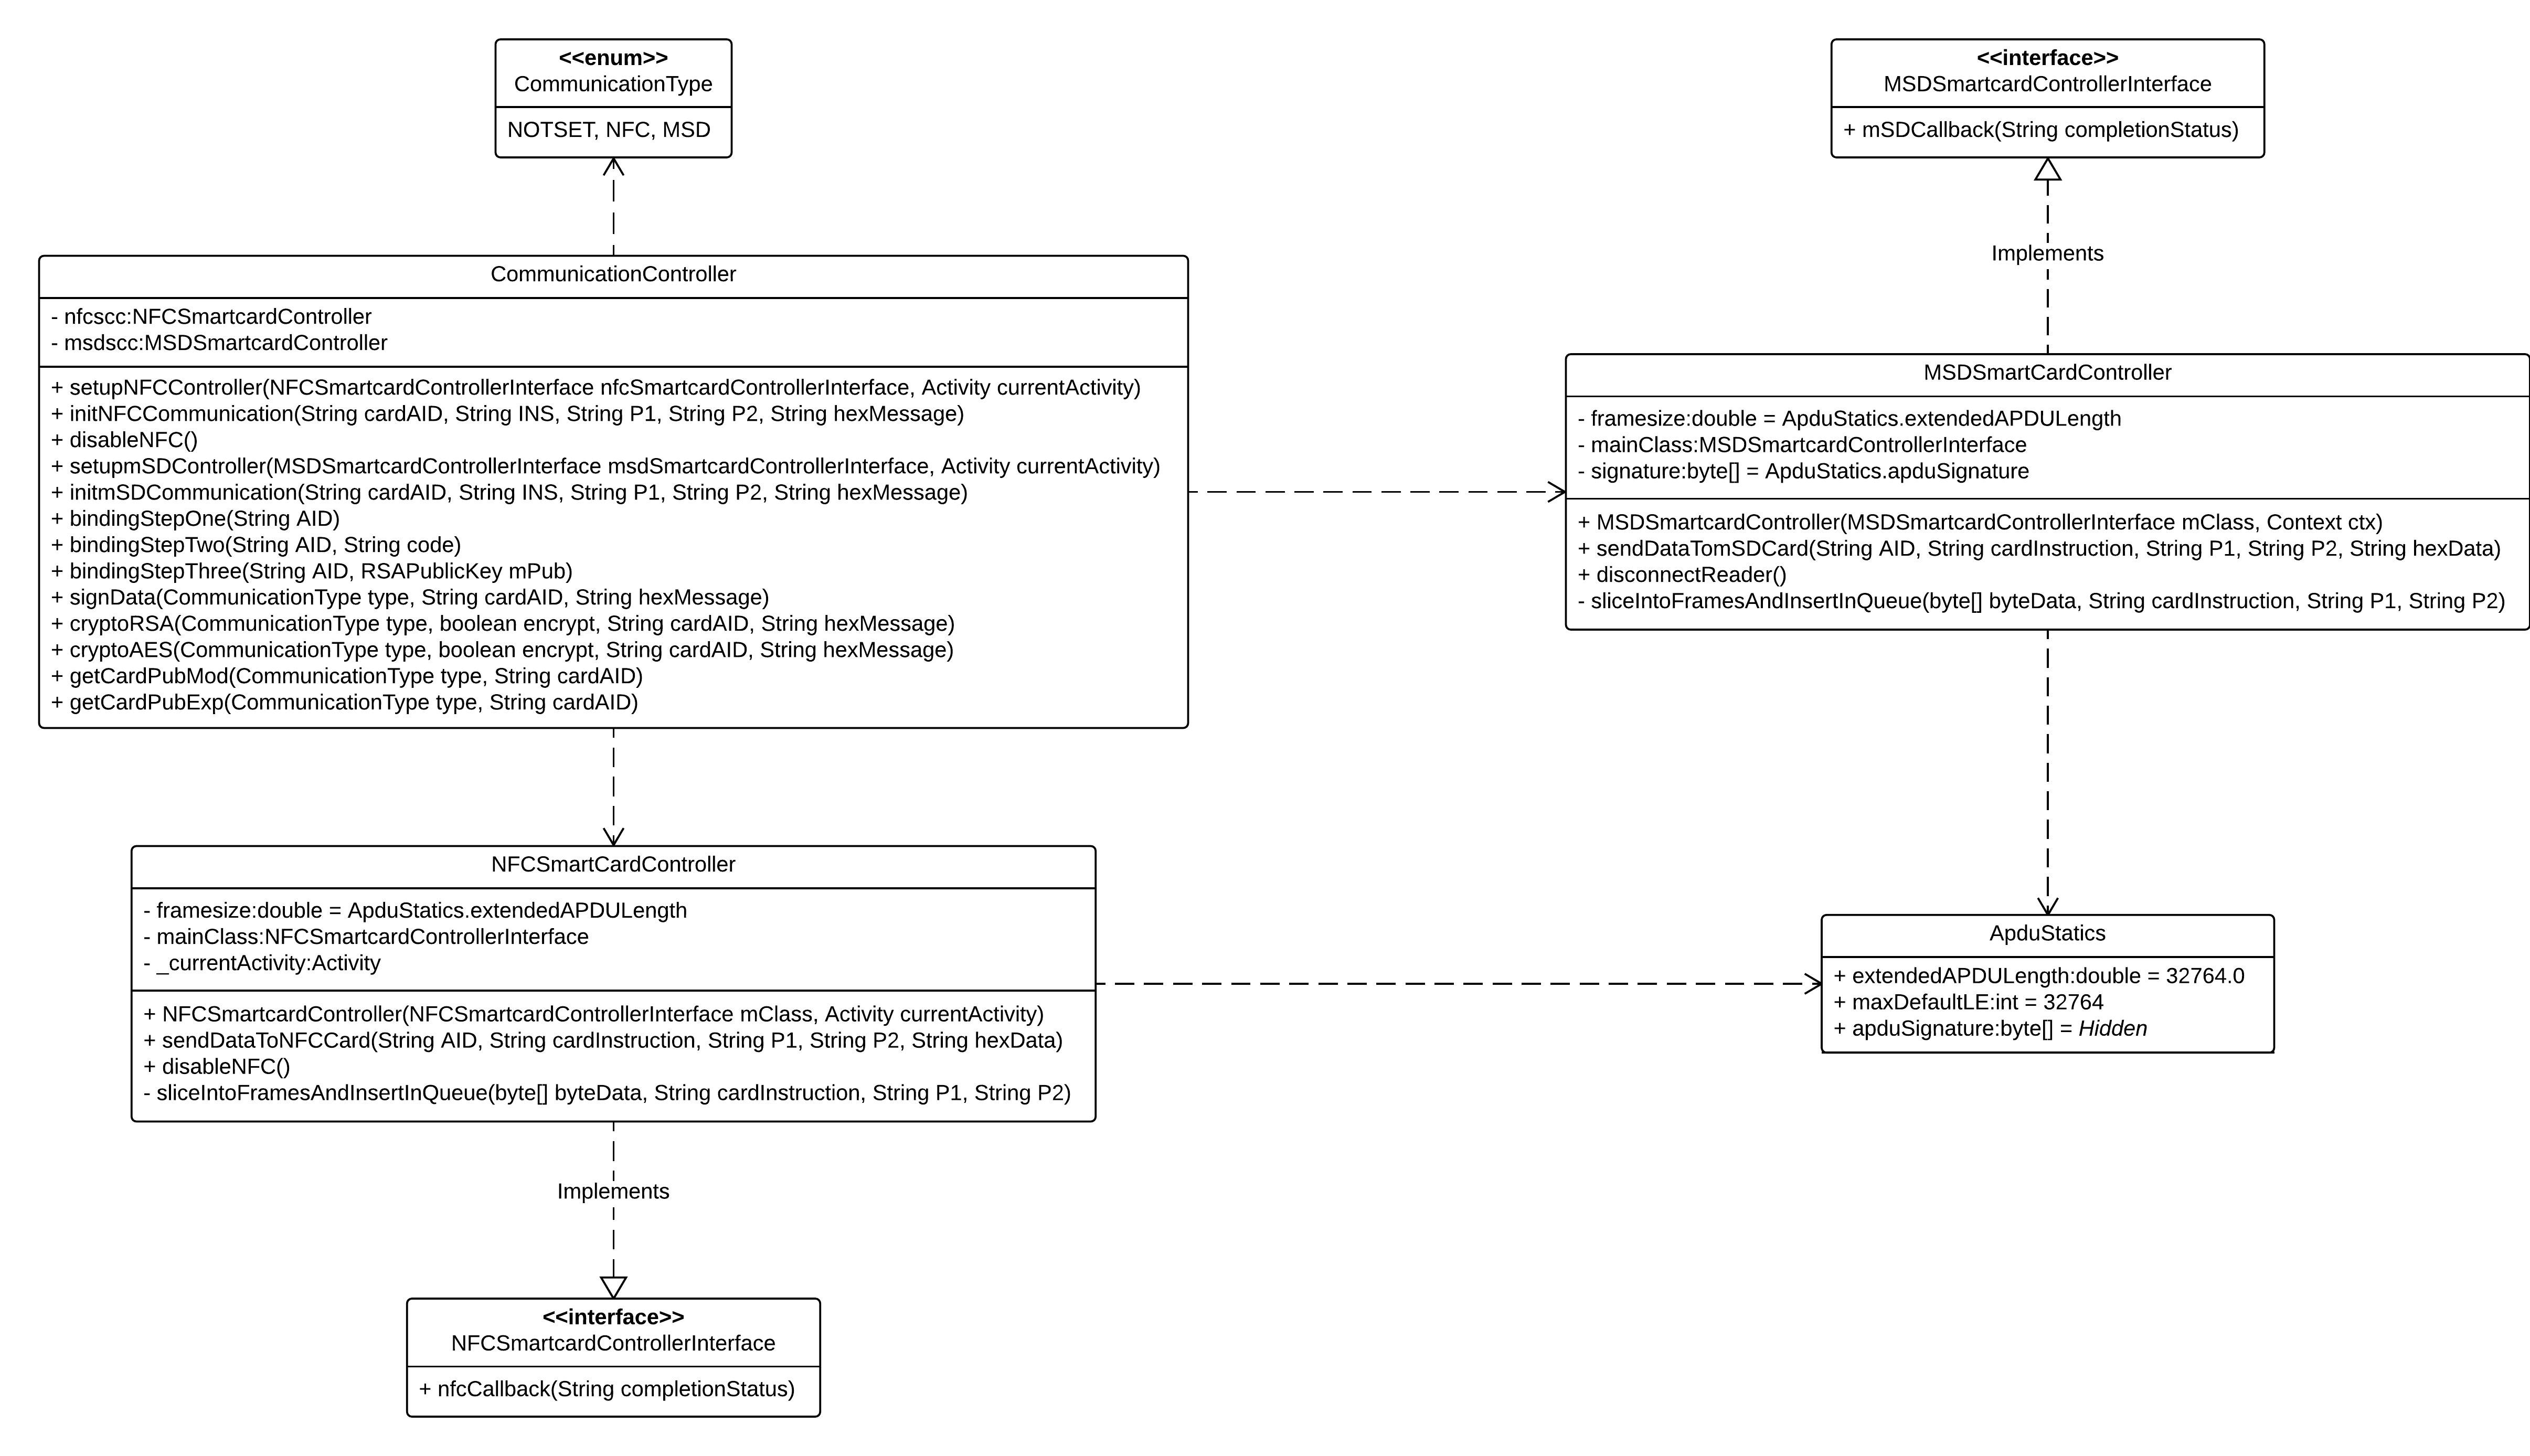
\includegraphics[width=0.95\textwidth]{images/Class_Diagram.png}
\end{figure}
The package diagram, figure \ref{fig:package}, shows how  the packages in the library are structured.

\begin{figure}[h!]
  \caption{Library package diagram.}
  \label{fig:package}
  \centering
    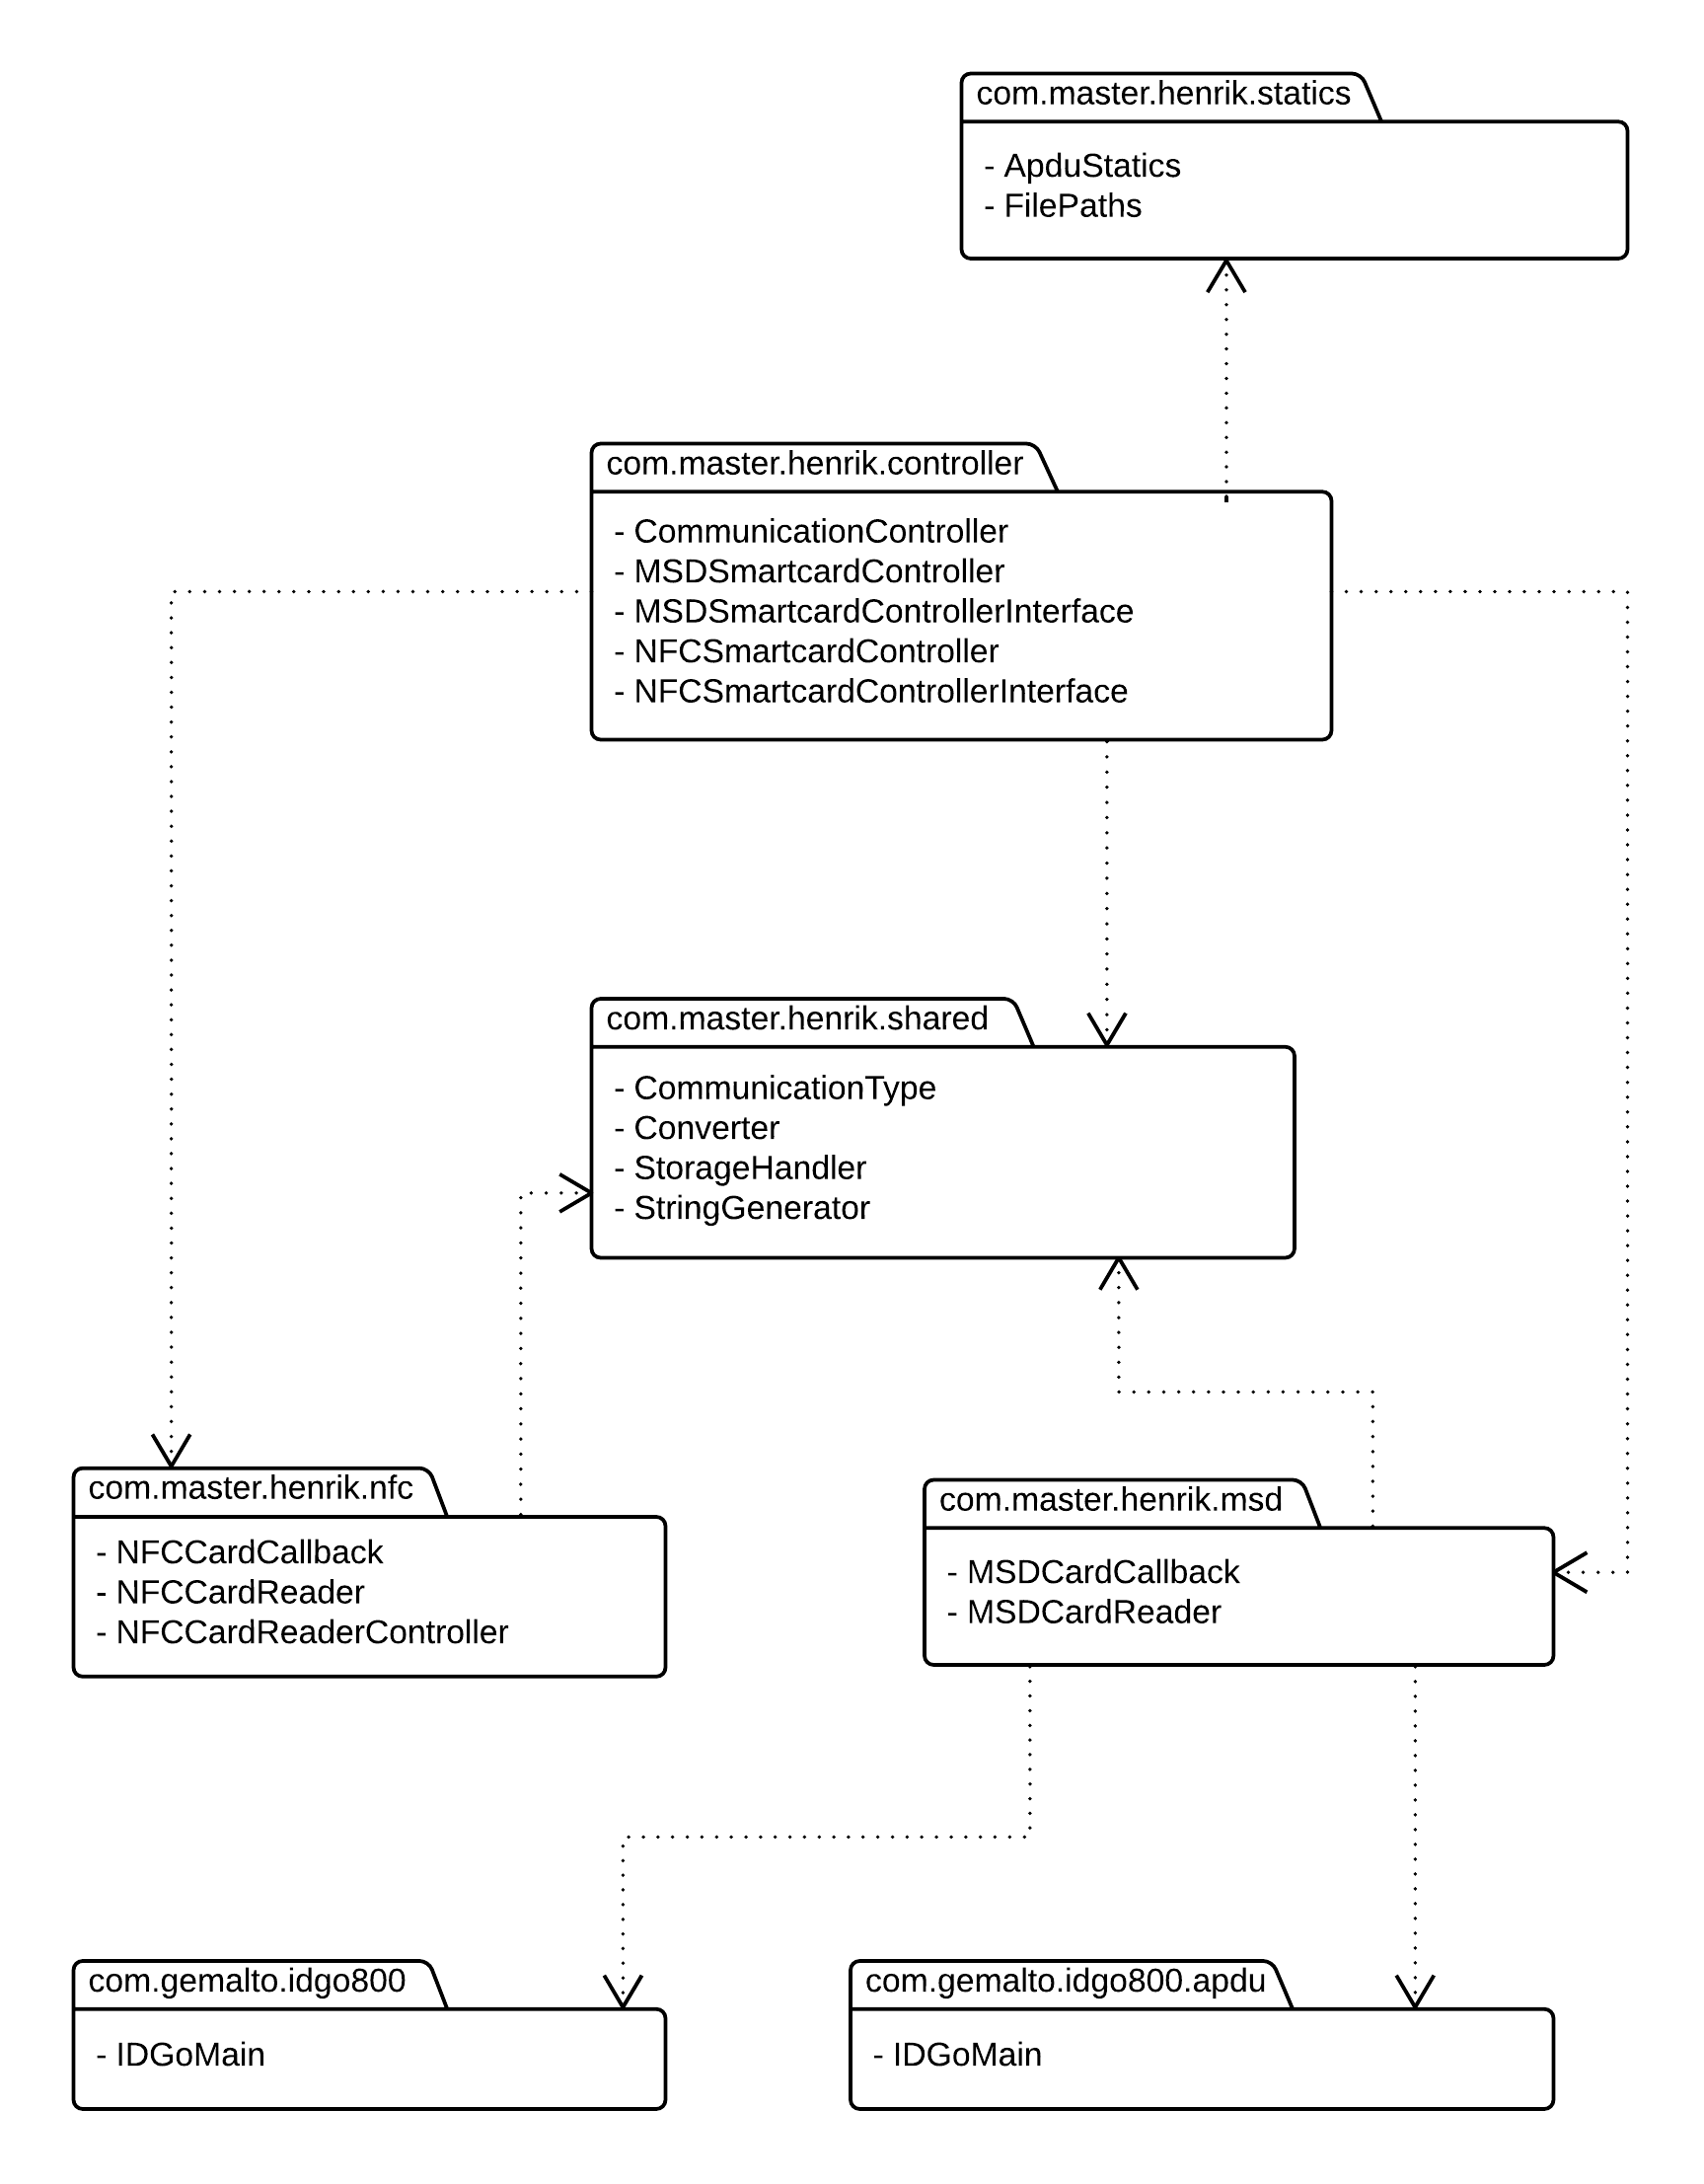
\includegraphics[width=0.95\textwidth]{images/package2.png}
\end{figure}


  % !TEX root = ../Article.tex
\chapter{Test Cases}
% !TEX root = ../Article.tex
\section{Setup}
In order to do research on how smart cards can have an impact on mobile data security and to perform an evaluation on how effective they are we need to have a proper test environment. We define ``proper test environment'' as an environment as close to reality as possible.
\subsection{Equipment}
\label{sec:equipment}

\paragraph{Test device}\mbox{}\\
The device we will be using for deploying the applications and performing tests on is considered to be a mid-range device. The device is a Sony Xperia M2 Aqua smartphone running Android 5.1.1 with the following relevant specifications:
\begin{itemize}
    \item Chipset: Qualcomm MSM8926-2 Snapdragon 400
    \item CPU: Quad-core 1.2 GHz Cortex-A7
    \item RAM: 1 GB
\end{itemize}
More information on the specifications of the phone can be found on  \newline
GSMArena.com \cite{sonym2}.

\paragraph{Java smart card}\mbox{}\\
We will be using two types of smart cards. The first type is a micro SD memory card (IDCore 8030 MicroSD card) as shown in figure \ref{fig:msdcard} produced by Gemalto. The reasoning for using this card for testing is that Gemalto delivers ready-to-use cards along with a framework for communicating with them. The cards we will be using have nothing pre-installed on them and we can freely deploy custom applications to the card. In order to use the provided framework we need a key provided by Gemalto which has a validity period of 120 days.

The second type of card we will be using is a plain hybrid smart card (ref. figure \ref{fig:nfccard}) with no pre-installed software which is also provided by Gemalto along with a standard card reader. In this case we are not reliant on the framework provided by Gemalto as Android has built in support for NFC communication in the standard SDK.

Both types of card are able to run the same application and thus makes it very convenient when comparing their performance against each other.

\iffalse %COMMENT

\subsection{Java card application}\mbox{}\\
The cards we have supports java card 2.2.2 and this is the version we will target. A natural question is "Why don't we target java card 3 and above?". Smart cards used for banking or handling other highly confidential data needs to be evaluated under the Common Criteria \cite{commoncriteria} standards. Potentionally we may handle confidential data and as a result we want smart cards with a Evaluation Assurance Level (EAL) 4 or above. Achieving EAL4 or above is an expensive and long process and the relatively few products have this certification. The micro SD card we have access to are certified with EAL5+, but only supports java card 2.2.2 \cite{gemaltoidgo8030}.

%TODO EAL list

A natural question we need to ask ourselves is: "Do we want Java card 3?"



\paragraph{Development environment}\mbox{}\\
In order to develop applications for the smart cards we will be using Eclipse 3.2 with java development kit version 1.6.45. In order to develop smart card applications more easily we will use the Eclipse-JCDE plugin \cite{eclipseJCDE} which provides a virtual runtime environment along with build tools.

We will be using GlobalPlatformPro (GP) \cite{globalplatform} to deploy and manage applets on the physical smart cards. GP is a command line tool and is compatible with our hybrid Gemalto card with reader as well as the micro SD card.

To test the smart card application that is deployed on the physical cards (without going through an Android application) we will be using pyApduTool \ref{pyapdutool}. pyApduTool is a tool for sending APDUs to a smart card through a card reader or memory card reader and lets us observe how the card behave when receiving and transmitting data.

\paragraph{Goal}\mbox{}\\
The goal of the smart card application was to create an autonomous and easy to extend platform for future tests. This resulted in an application split into three parts.

\paragraph{Initialization}\mbox{}\\
As described in section \ref{sec:javacard} all javacard applications must implement the method \texttt{Install}. \texttt{Install} invokes the constructor of the smart card and this is where all variables that need initialization are initialized. For instance if the smart card application needs to generate keys or random numbers this is where it is done as the constructor will be invoked only once. All buffers that needs to be used should also be initialized here to avoid allocating memory everytime the application is used.

\paragraph{Data processing}\mbox{}\\
In the mandatory \texttt{Process} method (refer to section \ref{sec:javacard}) all data processing takes place. First a built in method in the javacard API, \texttt{selectingApplet()}, is invoked. This method checks if the incoming APDU is a SELECT APDU and acts accordingly. If the incoming APDU is not a SELECT APDU the incoming APDU is copied to a new buffer for easier data manipulation. Next we use a switch statement switching over the second byte, INS, to determine which instruction we want to perform. After processing the data and performing the work we want to do (sign data, encrypt, etc.) we copy our response to the outgoing buffer.

\paragraph{Finalization}\mbox{}\\
At the end of the \texttt{Process} invokation we invoke the \texttt{Send} method which takes the data in the outgoing buffer, package it for sending and send it as a response APDU.

\paragraph{The result}\mbox{}\\
What we end up with is a test plattform where we are only concerned with declaring variables, initializing variables and writing code for the specific test case. Listing \ref{lst:pseudoCard} shows pseudocode for the java card application with the extendable areas highlighted.


\begin{lstlisting}[caption=Pseudo code for javacard test application., label=lst:pseudoCard,escapechar=!]
public class cardApplication extends Applet implements ExtendedLength{

    !\colorbox{highlight}{//Variable declarations}!

    private cardApplication() {
    	!\colorbox{highlight}{//Variable initialization}!
    }

    public void process(APDU apdu) {
    	//Process incoming APDU
        if (selectingApplet()) {
			return;
		}
        buff = apdu.getBuffer();

    	switch(buff[ISO7816.OFFSET_INS]){
            case 0x00:
            case 0x01:
            !\colorbox{highlight}{...}!
            case 0xff:
            default:

    	}
    	Send(apdu);
    }

    private void send(APDU apdu) {
    	//Package outgoing buffer
    	//Send response APDU
    }
}
\end{lstlisting}

\fi %UNCOMMENT

\iffalse %COMMENT

\subsection{Android application}
\paragraph{IDE}\mbox{}\\
Android Studio \cite{androidIDE} is the official IDE for Android application development. Android Studio is based on IntelliJ IDEA \cite{intelliJIDEA} and provides many automated tools for building, packaging and publishing Android applications.
\paragraph{3rd party libraries}\mbox{}\\
As mentioned in section \ref{sec:equipment} Gemalto provides a java library, IDGo800, for using their smart cards.

\begin{aquote}{Gemalto.com \cite{GemaltoIDGo800}}
"IDGo 800 for Mobiles is a cryptographic middleware that supports the Gemalto IDPrime cards and Secure Elements on Mobile platforms: Contact and contactless smart cards, MicroSD cards, UICC-SIM cards, embedded Secure Elements (eSE) and Trusted Execution Environment (TEE)."
\end{aquote}

The part of IDGo800 SDK we are interested in is very small and enables us to send custom APDUs to micro SD smart cards.

We will be using the "android.nfc" package in order to communicate with NFC smart cards. This package is included in the standard Android SDK which in turns means that all Android devices with a NFC reader and minimum API level 9 \cite{androidNFCminSDK} can use our library.

\paragraph{Application}\mbox{}\\
We used the same approach on the Android application as on the smart card application; an autonomous and easy to extend plattform for tests. This resulted in a new library, "smartcardlibrary",  which sole purpose is to transmit APDUs as easily as possible.

Smartcardlibrary has two main functions:
\begin{enumerate}
    \item{Communicate with NFC card}
    \item{Communicate with mSD card}
\end{enumerate}

To send APDUs to a smart card,\texttt{NFCSmartcardController} or\\ \texttt{MSDSmartcardController} (depending on smart card type) must be instantiated and the application must know the application identifier of the smart card application. Further the current activity must implement\\ \texttt{NfCSmartcardControllerInterface} or \texttt{MSDSmartcardControllerInterface} (depending on smart card type) in order to be notified when the transaction is complete. Listing \ref{lst:NFCLibraryExample} shows an example implementation on how an activity may utilize the library for NFC smart cards.

\begin{lstlisting}[caption=Java code example showing how to send and receive commands to a NFC smart card., label=lst:NFCLibraryExample,escapechar=å]

public class PayloadActivity extends AppCompatActivity implements NFCSmartcardControllerInterface {
    NFCSmartcardController nfcscc;
    ...

    private void initNFCCommunication(){
        if(nfcscc == null) {
            nfcscc = new NFCSmartcardController(this, this);
        }

        String AID = "0102030405060708090007";
        String hexMessage = "95404F3FB1";
        String cmd = "06";
        String p1 = "00";
        String p2 = "00";

        nfcscc.sendPayloadDataToNFCCard(AID, cmd, p1, p2, hexMessage);
    }

    å@Overrideå
    public void nfcCallback(final String completionStatus){
        if(!completionStatus.equals("OK")){
            return;
        }
        StorageHandler stHandler = new StorageHandler(getApplicationContext());
        String response = stHandler.readFromFileAppDir(FilePaths.tempStorageFileName);
    }
}

\end{lstlisting}

In order for the library to perform an asyncronous transaction the library will temporary save the responses from the cards to a file only accessible by the running application. To retrive the data the current activity should use the included \texttt{StorageHandler} class as used in listing \ref{lst:NFCLibraryExample}. The library also provides the class, \texttt{Converter}, for converting between Strings, hex and byte arrays.

Figure \ref{fig:package} shows how the library is structured and the entry point for applications is through the packages:

\begin{itemize}
    \item com.master.henrik.controller
    \item com.master.henrik.statics
    \item com.master.henrik.shared
\end{itemize}



\begin{figure}[h!]
  \caption{Library package diagram.}
  \label{fig:package}
  \centering
    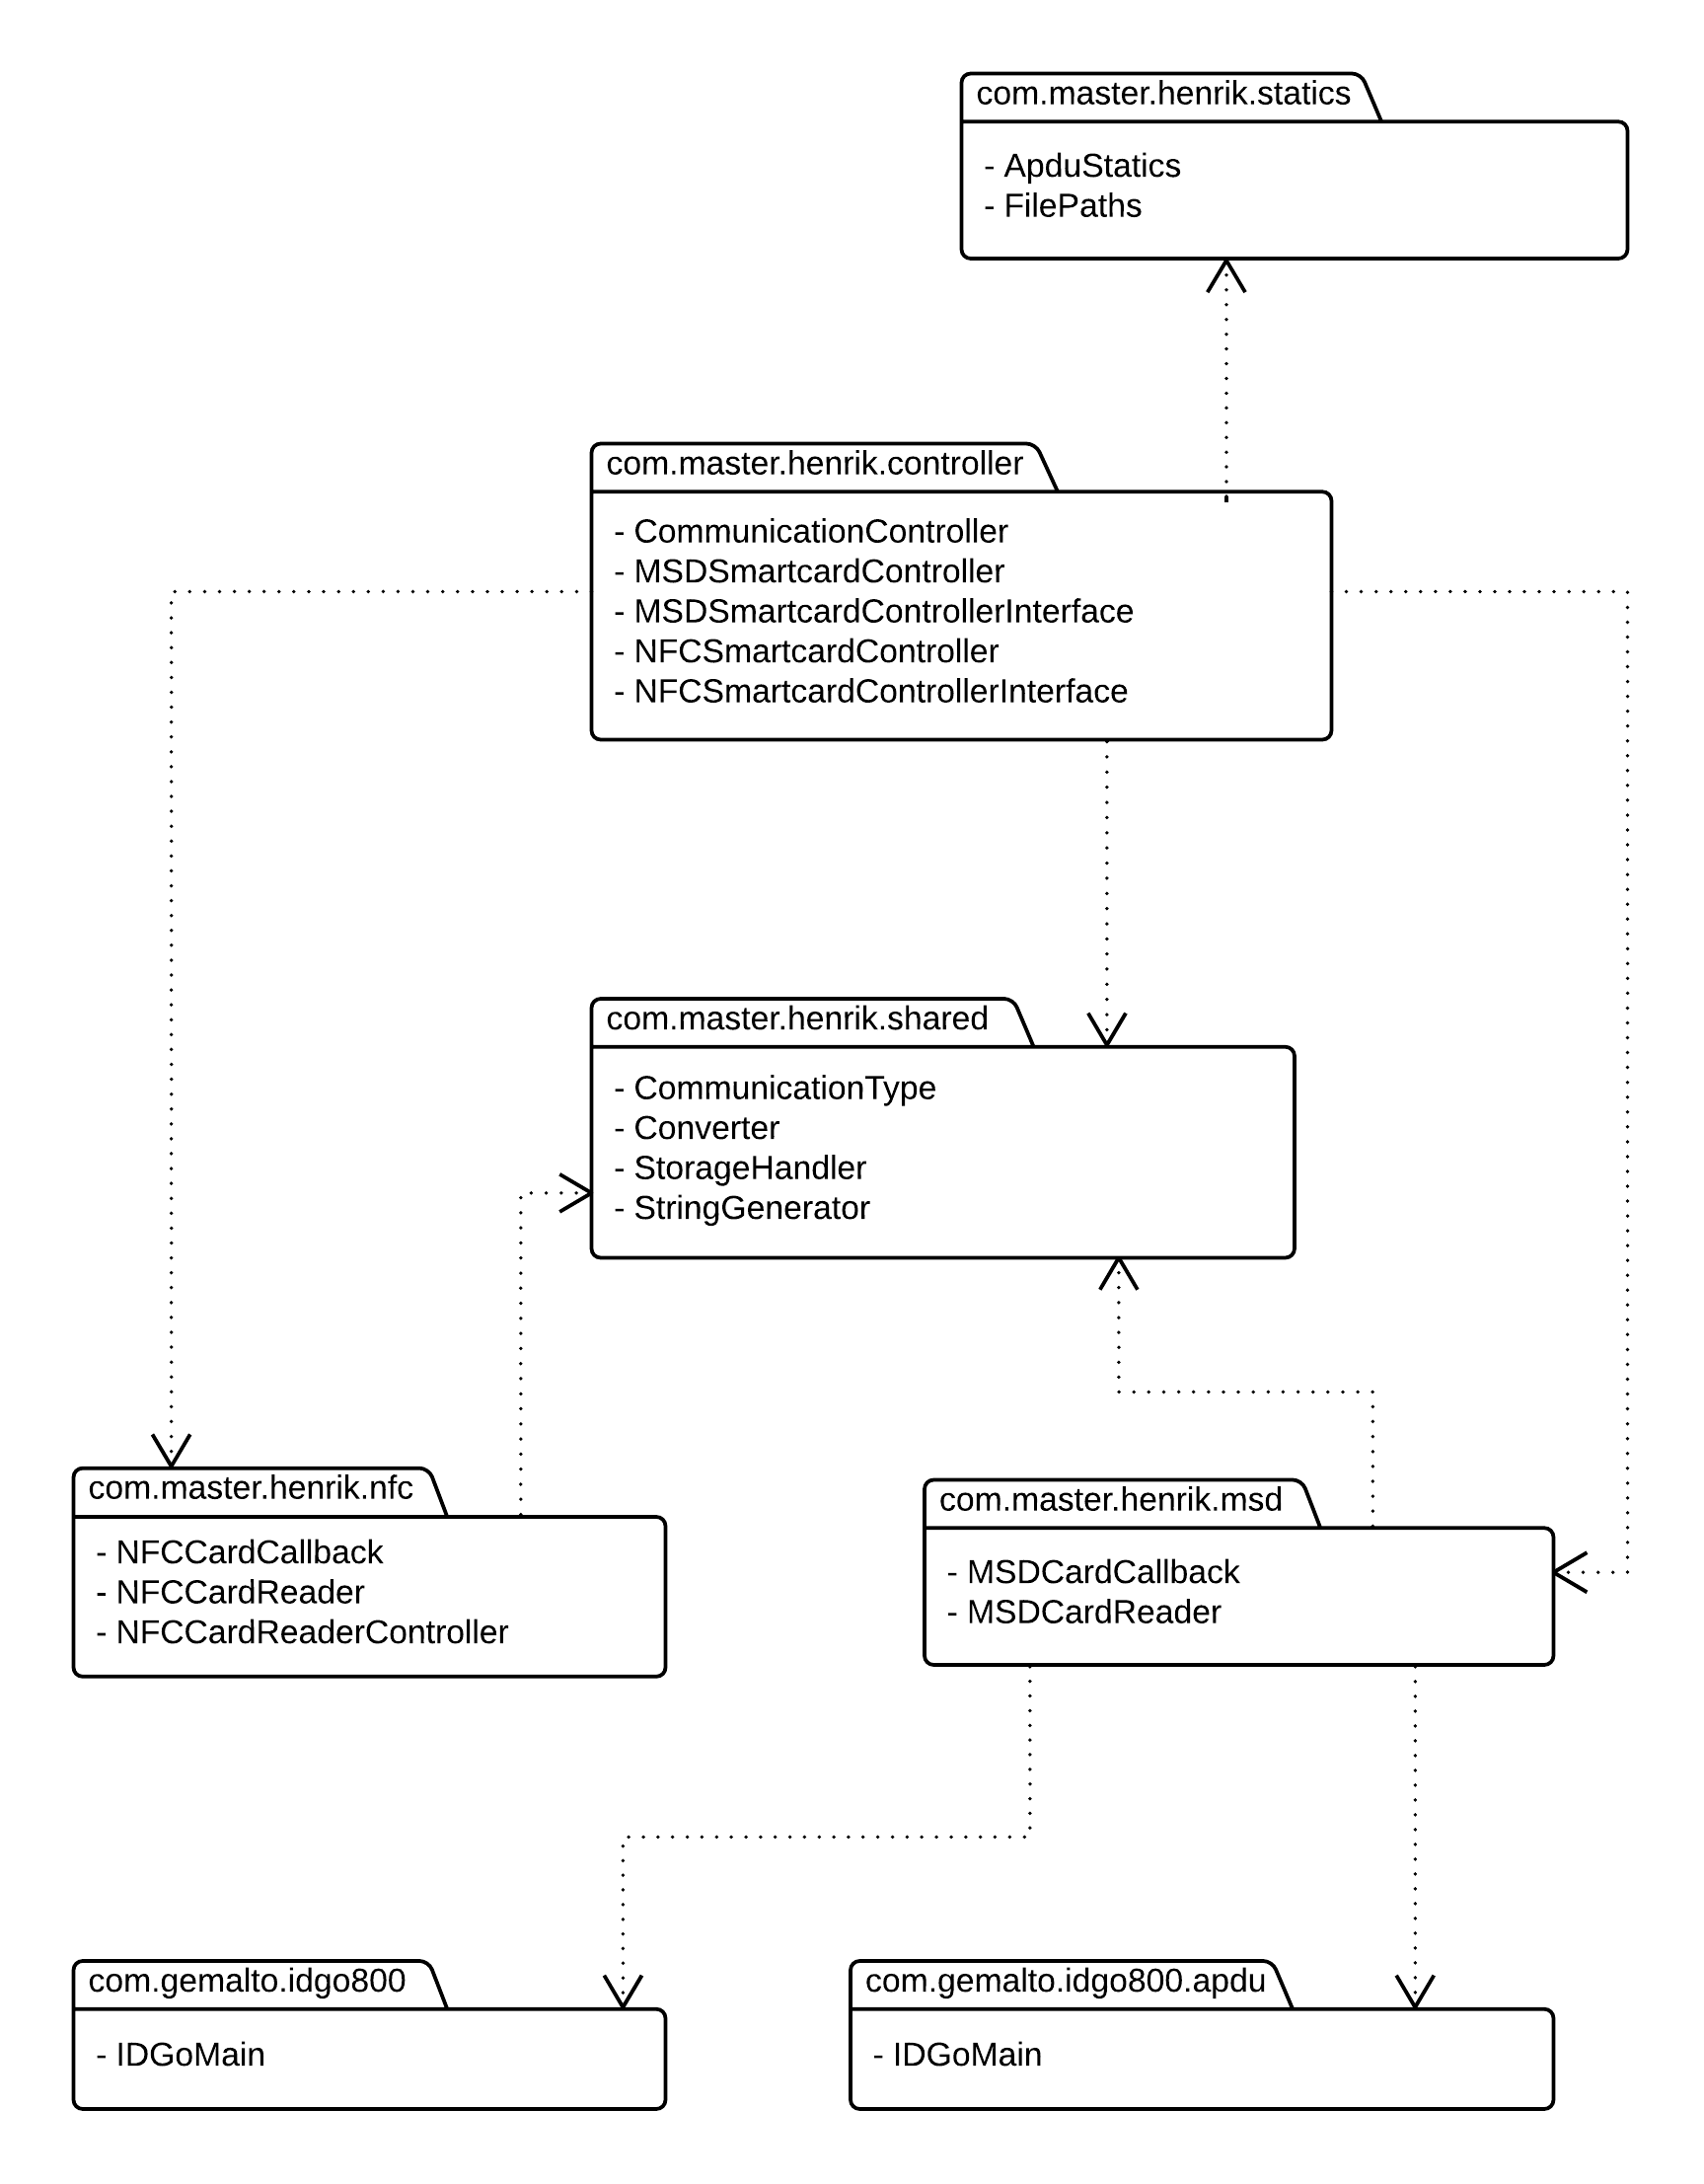
\includegraphics[width=0.95\textwidth]{images/package2.png}
\end{figure}

\fi %UNCOMMENT

\subsection{Limitations}
\label{sec:limitationsMSD}
When we started testing the implementation it became evident that the micro SD smart card we had did not support extended APDU. As a result we are not able to perform tests that involve micro SD cards and extended APDU.

% !TEX root = ../../Article.tex
\section{Data Transfer Speed}
\subsection{Description and Motivation}
Transfer speed is a very vital for part of the smart card interaction. If the smart card application or the transportation layer is incapable of handling large amounts of the data we will need to take that into account when examining the usability of smart cards. In order to test and eliminate as many variables as possible the smart card is programmed to receive data, copy the incoming data to the buffer and send the exact same data in return. Figure \ref{fig:nfcDataflowTest} describes this process using an NFC card as a platform for the Java Card Applet.

\begin{figure}[h!]
  \caption{Data flow of data transfer speed test for NFC.}
  \label{fig:nfcDataflowTest}
  \centering
    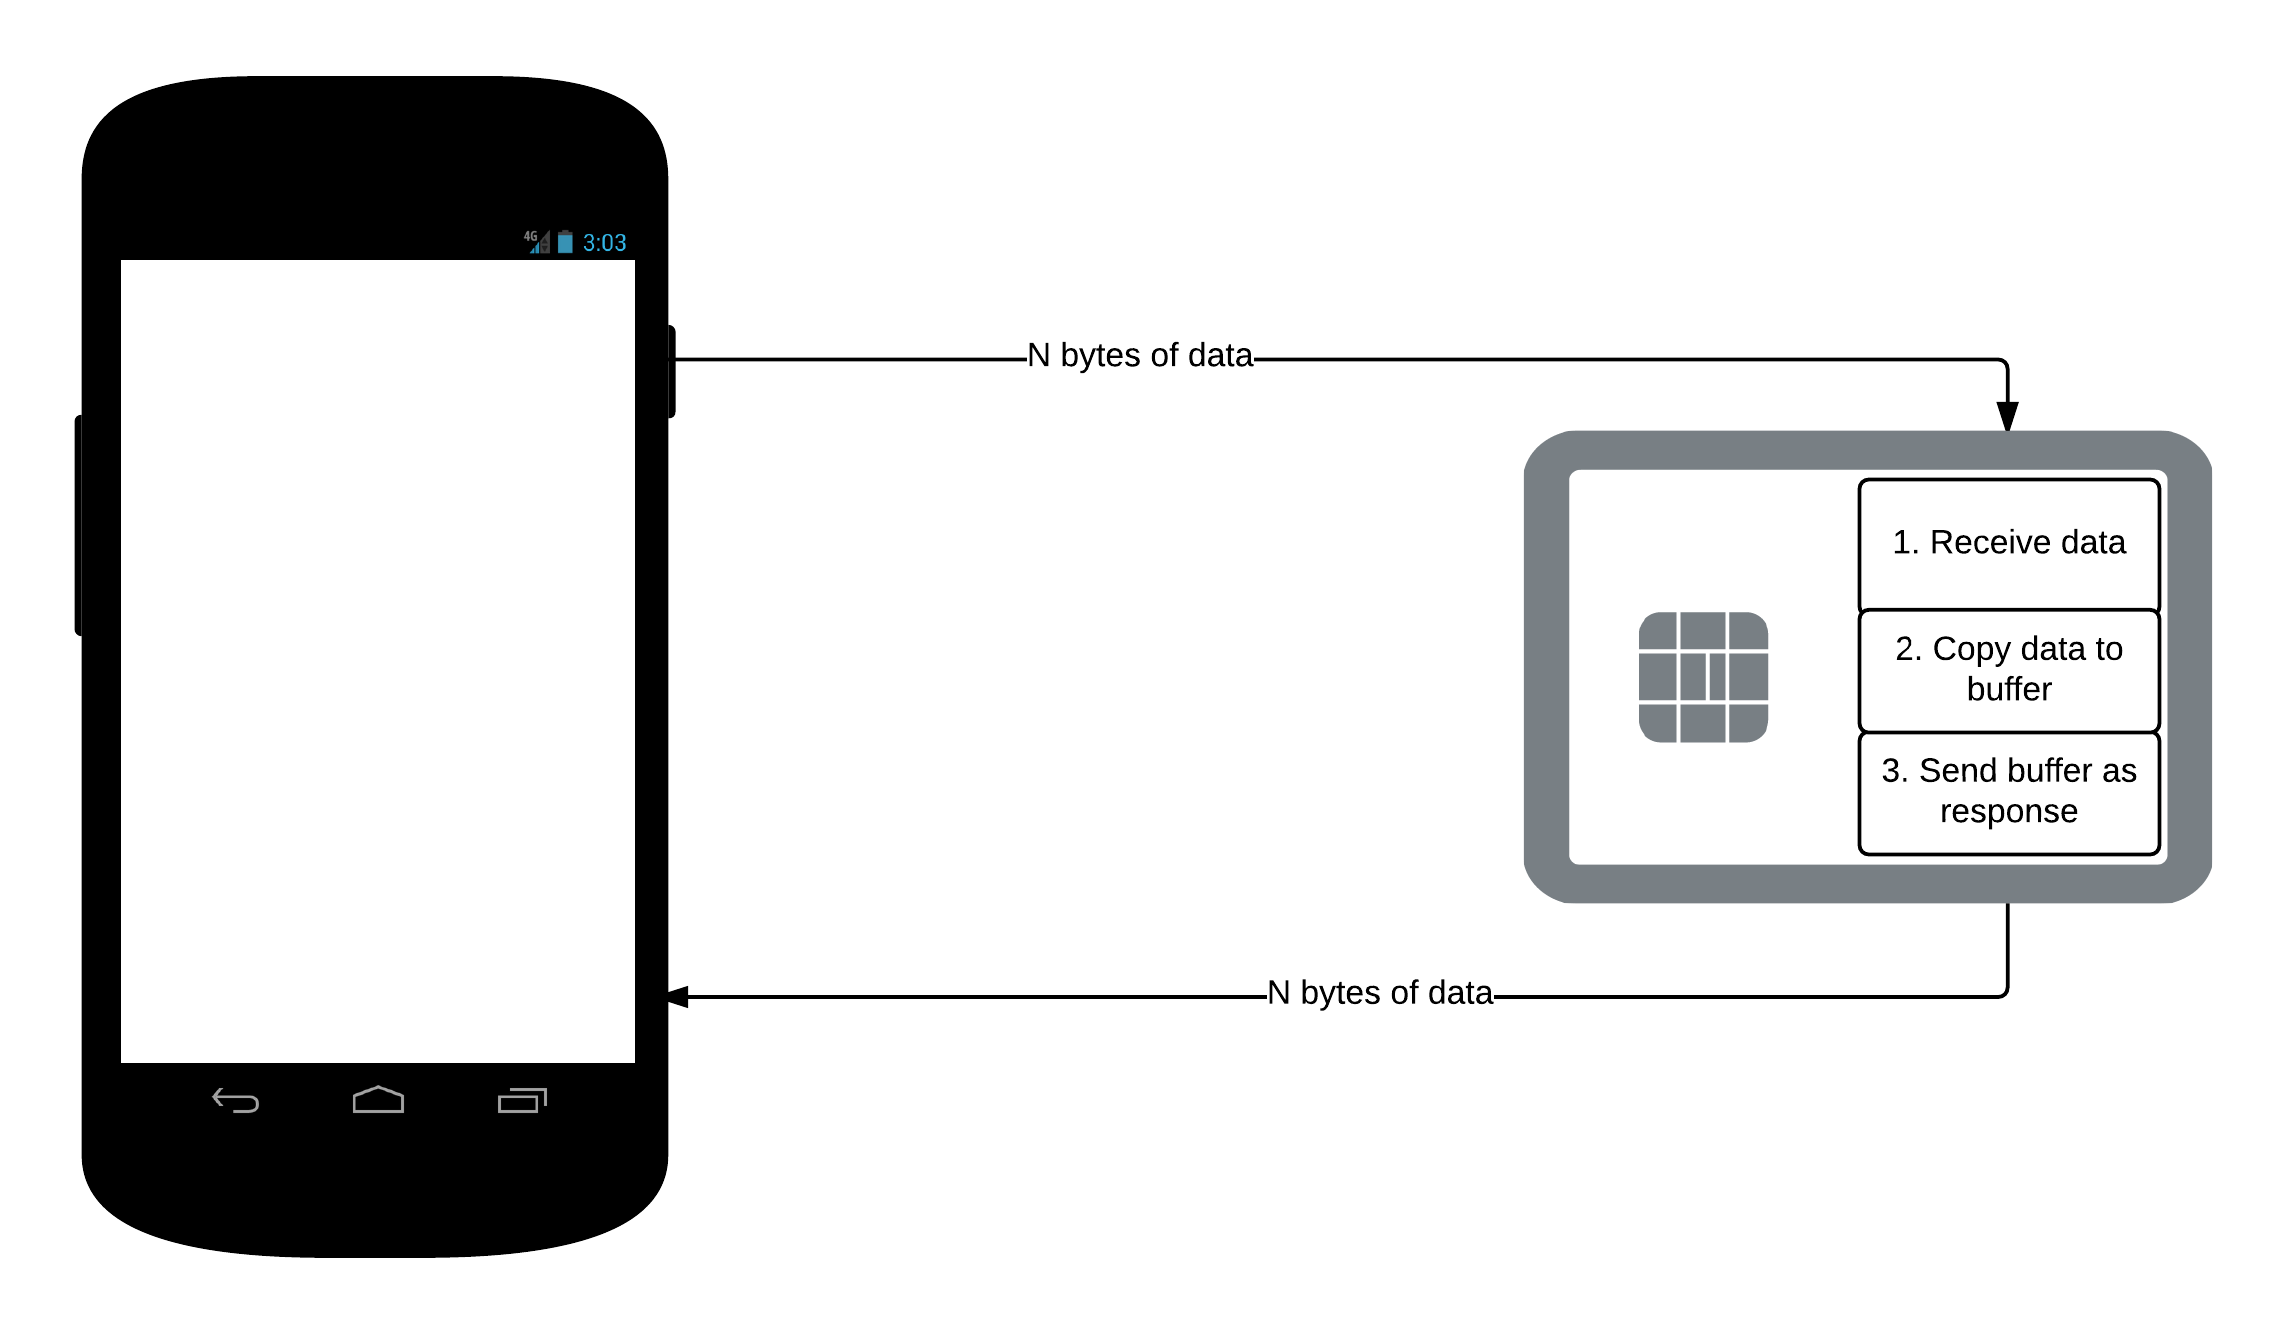
\includegraphics[width=0.95\textwidth]{images/NFCTransferTest.png}
\end{figure}

\subsection{Tests and Results}
\paragraph{NFC}\mbox{}\\
\begin{table}[h!]
\caption{Table of NFC transfer speed test.}
\label{tbl:nfcspeed}
\centering

    \begin{tabular}{ | l | r | r | r |}
        \hline
        \thead{Data size (byte)}
        & \thead{T1}
        & \thead{T2}
        & \thead{T3} \\ \hline

        10000 & 3,8s & 4,1s & 3,6s \\ \hline
        100000 & 41,3s & 35,0s & 24,7s \\ \hline
        1000000 & 602,1s & 361,3s & 235,1s \\ \hline

    \end{tabular}

\end{table}

%\vspace{1cm}
\begin{figure}[h!]

    \caption{Graphical representation of table \ref{tbl:nfcspeed}.}
    \label{fig:nfcgraph}
    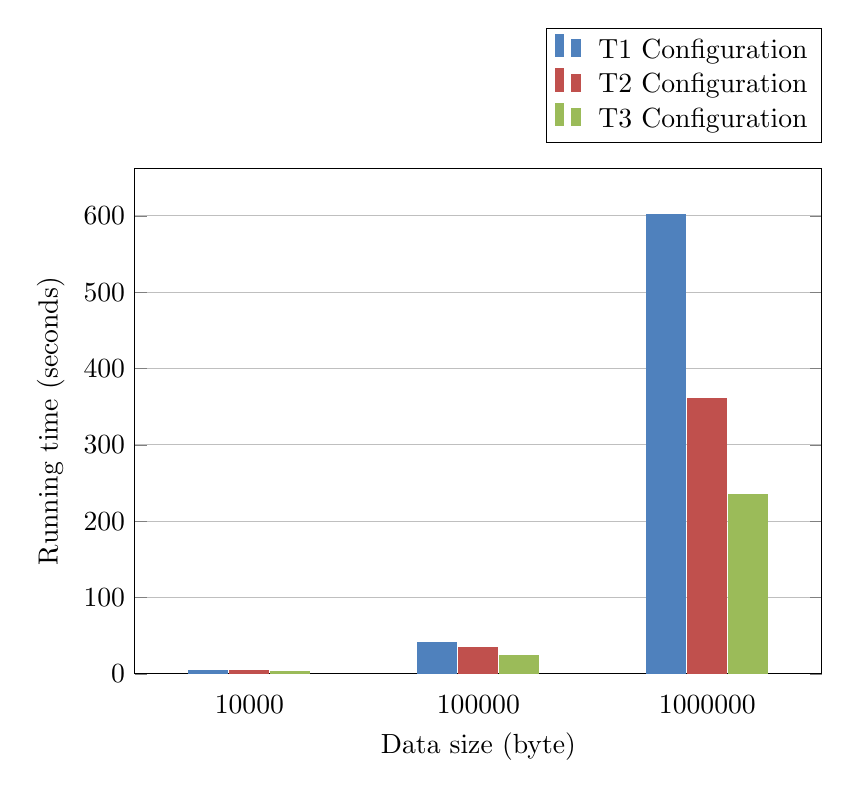
\begin{tikzpicture}
        \centering
            \begin{axis}[
                width  = 0.85*\textwidth,
                height = 8cm,
                major x tick style = transparent,
                ybar=2*\pgflinewidth,
                bar width=14pt,
                ymajorgrids = true,
                ylabel = {Running time (seconds)},
                xlabel = {Data size (byte)},
                symbolic x coords={10000, 100000, 1000000},
                xtick = data,
                scaled y ticks = false,
                enlarge x limits=0.25,
                ymin=0,
                legend cell align=left,
                legend style={
                        at={(1,1.05)},
                        anchor=south east,
                        column sep=1ex
                }
            ]
                \addplot[style={bblue,fill=bblue,mark=none}]
                    coordinates {(10000, 3.89) (100000, 41.29) (1000000, 602)};

                \addplot[style={rred,fill=rred,mark=none}]
                     coordinates {(10000, 4) (100000, 35) (1000000, 361)};

                \addplot[style={ggreen,fill=ggreen,mark=none}]
                     coordinates {(10000, 3.6) (100000, 24) (1000000, 235)};

                \legend{T1 Configuration,T2 Configuration,T3 Configuration}


            \end{axis}
    \end{tikzpicture}
\end{figure}


\newpage
\paragraph{Micro SD}\mbox{}\\
T1 configuration, from NFC was dropped when testing transfers speed for micro SD as it became clear from previous tests on NFC that T1 is vastly inferior to T2 and T3. A non-asyncronous (not using streams) Android application is not representative of the "real-world" and we decided on not pursuing further test results using this configuration.

T2 configuration consist of the Android application sending data to the smart card application using frames of size 255 byte until all data is sent. Simultaneously the responses are written to an internal file using FileOutputStream (provided by the standard Java library).

We were not able to test T3 configuration as explained in section \ref{sec:limitationsMSD}.

\begin{table}[h!]
\caption{Table of micro SD transfer speed test.}
\label{tbl:msdspeed}
\centering

    \begin{tabular}{ | l | r | r |}
        \hline
        \thead{Data size (byte)}
        & \thead{T2}
        & \thead{T3} \\ \hline

        10000  & 3,18s & N/A s \\ \hline
        100000 & 16,14s & N/A s \\ \hline
        1000000 & 142s & N/A s \\ \hline

    \end{tabular}

\end{table}


\newpage
\subsection{Conclusion}
From table \ref{tbl:nfcspeed} and figure \ref{fig:nfcgraph} we can learn that we are able to optimize the data transfer and processing speed between the Android application and the NFC card. It is also clear that when we are transmitting low amounts of data there is virtually no difference between the configurations; T1, T2 and T3. The differences are more prominent when the data amounts increase. Even though we achieved an improvement of approximately 60 \% from T1 to T3 when sending 1 MB of data, the process is still time consuming.

If we compare the test results for T2 configuration on the NFC card and micro SD card we can clearly see an improvement on the micro SD card. The micro SD card had a ~60 \%  better running time over the NFC card when sending 1 MB of data. Although we were not able to test configuration T3 on the micro SD card, results point in the direction of micro SD cards having better performance than NFC cards. We are not able to confirm this and thus cannot be treated as a fact.

Even though we are able to optimize and improve data transfer speeds, we are still very far from transferring and processing large amounts of data quickly. We have to take this into account when evaluating areas of use for the smart card. Transfer and processing speed rules out many areas concerning large amounts of data, such as full data encryption.


% !TEX root = ../../Article.tex
\section{Symmetric-key Cryptography}
\label{sec:symmetricTest}
\subsection{Description and Motivation}
We want to discover the encryption abilities on the smart card and decide if it is feasible to let the smart card handle the encryption of confidential data. From the smart card documentation we know that we are able to use AES to encrypt data, but we do not know how long it will take to encrypt the data. We will need to perform a run time tests with different amounts of data in order to determine the performance of the smart card.

\subsection{Test setup}
The framework we are using is designed around extended APDU and the test platform we have designed in Java Card utilizes extended APDU. As a result we are not able to use the micro SD cards (as described in section \ref{sec:limitationsMSD}) and we will be using the NFC smart cards.

The encryption algorithm we will use is AES cipher algorithm with block chaining (CBC). The version of Java Card that we are using along with our smart cards limits us to using 128 bits keys and no padding. More specifically the only working AES algorithm from javacard is \texttt{ALG\_AES\_BLOCK\_128\_CBC\_NOPAD}, even though the Java Card documentation for \texttt{Cipher} supports more algorithms \cite{javacardCipher}. Others have encountered the same discrepancy \cite{javacardCipherFail} suggesting that only three of the twelve supported algorithms works, but there exists no official information on the issue.

\texttt{ALG\_AES\_BLOCK\_128\_CBC\_NOPAD} is as the name suggest an algorithm with no padding. The block size the AES algorithm expects is 16 byte and as a result we will need to pad the data ourselves on the mobile device.

\subsection{Results}
% !TEX root = ../Article.tex

\begin{table}[h!]
\caption{Table of AES encryption speed test.}
\label{tbl:AESSpeed}
\centering

    \begin{tabular}{ | l | r |}
        \hline
        \thead{Data size (byte)}
        & \thead{Elapsed time} \\ \hline

        10000  & 20,18s \\ \hline
        32000  & 61,81s \\ \hline
        100000 & 183,78s \\ \hline
        1000000 & 1835,49s \\ \hline

    \end{tabular}

\end{table}

\begin{figure}[h!]

    \caption{Graphical representation of table \ref{tbl:AESSpeed}.}
    \label{fig:nfcgraph}
    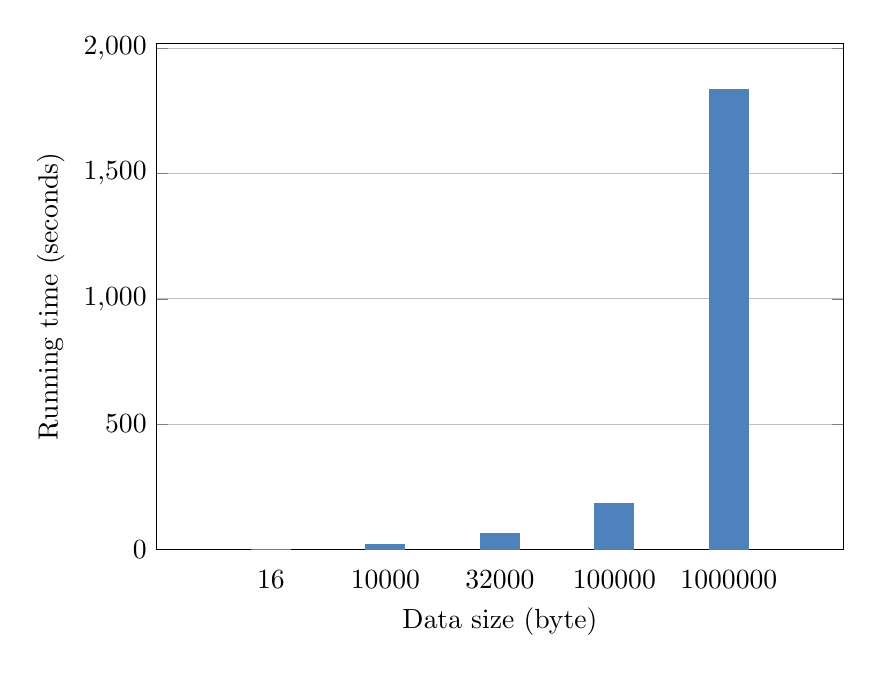
\begin{tikzpicture}
        \centering
            \begin{axis}[
                width  = 0.85*\textwidth,
                height = 8cm,
                major x tick style = transparent,
                ybar=2*\pgflinewidth,
                bar width=14pt,
                ymajorgrids = true,
                ylabel = {Running time (seconds)},
                xlabel = {Data size (byte)},
                symbolic x coords={16, 10000, 32000, 100000, 1000000},
                xtick = data,
                scaled y ticks = false,
                enlarge x limits=0.25,
                ymin=0,
                legend cell align=left,
                legend style={
                        at={(1,1.05)},
                        anchor=south east,
                        column sep=1ex
                }
            ]
                \addplot[style={bblue,fill=bblue,mark=none}]
                    coordinates {(16, 0.15) (10000, 20.62) (32000, 61) (100000, 183) (1000000, 1835)};
            \end{axis}
    \end{tikzpicture}
\end{figure}

\subsection{Conclusion}
From the test results we can learn that encrypting data on the NFC smart card takes a lot of time. Encrypting 1MB of data uses approximately 30 minutes, which from a real world perspective is an unacceptable amount of time. Using the NFC smart card for full encryption of user data is in other words not achievable and we will need to look for other options for encryption.

Encrypting 16 bytes of data uses 0,15 seconds. A use for the encryption capabilities on the smart card may be to encrypt small amounts of data such as GPS coordinates. GPS coordinates can be represented by only 16 bytes (depending on accuracy). One could also imagine that we will only need to encrypt parts of a document, and as long as we keep the data size small we can let the smart card do the encryption.


\section{Public-key Cryptography}
\subsection{Description and Motivation}
\subsection{Tests and Results}
\subsection{Conclusion}

  % !TEX root = ../Article.tex
\chapter{Conclusion}
\label{ch:conclusion}

\section{Research questions}
\begin{itemize}
  \item \textit{``What are the limitiations of smart cards in the context of hardware?''}\\
  There hardware limitations of smart cards are very dependent on which smart card you are using. Generally smart cards are limited when it comes to computing power and this has a huge effect on how resource intensive operations you are able to perform on the smart card. Secure cryptography are very resource intensive and our test results show that encrypting large amounts of data is unfeasible, both for public-key cryptography (RSA) and symmetric-key cryptography (AES). We performed tests regarding transfer speed and they show that the throughput of input/output are limited and that we often run the risk of running out of memory with large amounts of data.
  \item \textit{``What are the limitiations of smart cards applications?''}\\
  We opted for using JavaCard as our programming language. Our version of JavaCard does not support advanced datatypes. This combined with the fact that all data being sent to/from the smart card is byte values creates a rigid environment with hardcoded values. JavaCard does not support standard garbage collection and thus applications needs to be extra careful when allocating memory.
  \item \textit{``What are the types of use cases we are able to solve and strengthen the security of using smart cards?''}\\
  Even though smart cards have some areas with limitations we are able to identify use cases where smart cards can be applicable. In use cases involving cryptography a smart card can store the keys securely aswell as encrypt/decrypt small amounts of data. Due to the fact that smart cards are tamper proof, meaning that you are not able to extract data (keys), we are confident that smart cards can alleviate threats such as stolen mobile devices and insecure communication channels.\mbox{}\\\\  We believe that smart cards can add an extra layer of security for areas that are already solved. In this thesis we described and analyzed a solution where we used smart cards as a basis for policy enforcement. Our comprehension is that this type of solution in conjuction with traditional policy enforcement systems will take security to a new level.
\end{itemize}

\section{Experience}
After working with smart cards for roughly one year we have made quite a few experiences that are worth sharing.

\paragraph{Getting started with smart card programming}\mbox{}\\
Getting started with smart card programming can be difficult. After a few years with object-oriented programming most programmers will start to get comfortable using ``quality of life'' classes such as \texttt{ArrayList} and \texttt{Enum}. That world gets turned up-side down when moving to Java Card. One is  thrown back to an older Java version and as a programmer you will need to rethink how you solve problems and structure solutions. Most notable is the fact that all incoming data is in the form of a \texttt{byte} array that must be mapped to the correct datatypes. Missing functionality such as standard Java garbage collection and standard data types (\texttt{int}, \texttt{double}, etc.), makes Java Card programming cumbersome and requires time to adapt to.

\paragraph{Debugging smart card applications}\mbox{}\\
Debugging smart card applications differs from standard debugging. Normally when debugging you are able to insert breakpoint, inspect variables and monitor resource usage. The nature of smart cards is to be a secure and closed environment and thus it is hard to monitor how an application behaves. The debugging method we have available is: deploy the application, send data to it and see what the response is. If the response does not match expected output the best way to debug is creating manual breakpoints, i.e., add a line of code returning the value of variables and try to figure out where the error might be. Sometimes the smart card encounter runtime exceptions and sends a 2 byte response that is mapped to an error message \cite{javacardErrors}.

This type of debugging environment is exhausting and is requires a lot of resources. Often we spent time trying to pinpoint an error only to later found out that the error code we got had nothing to with the actual problem. This was especially noteable with errors regarding memory usage. One of the best advices concerning smart card debugging is: ``Test often with a big array of test data.''.

\paragraph{JavaCard documentation}\mbox{}\\
The documentation available is very technical. This is not by any means a bad thing, but it does require developers to understand smart cards fully before using the documentation. When comparing Android and JavaCard documentation, it is very apparent that Google has put a lot of effort into having an educational approach to the concepts before diving into the technical aspects. In the JavaCard documentation there are very few examples of usage, and we spent a lot of time trying to figure out how to properly use classes and methods.

The gap between software and hardware is very apparent in the JavaCard documentation. We often encountered functionality that was supposed to work, but did not work on our smart cards. The result of this was that when we encountered bugs, we did not know if it was a programming mistake or simply not supported by our smart cards. The best example of this was when we tried to use the \texttt{Cipher} class with algorithms that proved to not work on our smart cards (section \ref{sec:symmetricTest}).

\paragraph{Deploying smart card applications}\mbox{}\\
Deploying smart card applications to a smart card is a time consuming task. This became very apparent when working with micro SD smart cards. Deploying a new version to micro SD required us to: remove mSD from mobile device, insert mSD into computer, run install script, wait on install script to finish, insert mSD into mobile device. Following this procedure once in a while is not a big inconvenience, but in context of debugging it become very tideous to spend 1,5 minutes switching around the mSD card and waiting for the install script.

\section{Future work}
\label{sec:future}
The research we have presented in this thesis are a good starting point for developing custom security applications on the Android platform in conjunction with smart cards. The test cases we have looked into point to that micro SD cards have better performance than NFC cards, but our micro SD cards did not support extended APDUs and thus we cannot confirm that micro SD are better than NFC cards. More work on micro SD cards must be performed in order to confirm these suspicions.

We encountered numerous bugs and limitations when working with smart cards which we did not initially predict, and as a result the Android library and the smart card application is not as polished and refined as we had hoped it would be. This includes adding more pre-implemented functionality, refactoring code to be more readable and optimize code to achieve better performance. Additionally we believe it would be beneficial to look at the possibility of not being dependent on the Gemalto framework for micro SD card communication \cite[\textit{SEEK for Android}]{SEEK}.

Our evaluations of the proposed solutions are based on protocol analysis and proof of concept. It would be beneficial to perform penetration tests on the outlined solutions to confirm that: \textit{a)} We are able to implement all parts of the solution. \textit{b)} We can show that the solution is methodically tested against known attacks in today's society.


  % !TEX root = ../Article.tex
\newpage
\appendix
% !TEX root = ../../Article.tex
\chapter{Java Card code}
\label{app:A}
\begin{lstlisting}[caption=SecureCard.java.,breaklines=true,breakatwhitespace=false, label=lst:SecureCard,escapechar=!]
package henrik;

import javacard.framework.APDU;
import javacard.framework.Applet;
import javacard.framework.ISO7816;
import javacard.framework.ISOException;
import javacard.framework.OwnerPIN;
import javacard.framework.Util;
import javacard.security.CryptoException;
import javacard.security.KeyBuilder;
import javacard.security.KeyPair;
import javacard.security.RSAPrivateKey;
import javacard.security.RSAPublicKey;
import javacard.security.Signature;
import javacard.security.AESKey;
import javacardx.apdu.ExtendedLength;
import javacardx.crypto.*;
import javacard.security.*;
import javacard.framework.JCSystem;

public class SecureCard extends Applet implements ExtendedLength{
	//Try to allocate all variable here and do not create new ones
	//The Public/Private key pair that this card will use
	private KeyPair keys;
	private KeyPair sKeys; //PLACEHOLDER
	//Signature object to sign with card private key
	private Signature sig;
	//Card Public key
	private RSAPublicKey uPub;
    //Card Private key
	private RSAPrivateKey uPrv;
    //	To store data to be sent beck to host application
	byte[] output = new byte[32767];
	//for temporary storing data before copying into output
	byte[] buff2 = new byte[2];
	//For bigger data
	byte[] bigArray;
	//To store the size of the output buffer
	short size;
	//Length of signature or other short values
	short len;
	//Size of modulus and signature
	final short keysize=64;

	//Predefined Commands
	private final byte SEND_U_PUB_MOD=(byte) 0x01;
	private final byte SEND_U_PUB_EXP=(byte) 0x02;
	private final byte SIGN=(byte) 0x03;
	private final byte BINDING=(byte) 0x05;
	private final byte RSACRYPTO=(byte) 0x06;
	private final byte REFLECT=(byte) 0x08;
	private final byte AESCRYPTO=(byte) 0x09;



	//Cryptography
	Cipher cipherRSA;
	Cipher cipherAES;
	byte[] cryptoBuffer;// = new byte[32767];

	AESKey aesKey;
	RandomData randomData;
	byte[] rnd;


	short policy13Offset = 6;


	//Binding
	byte pinIsPresentFlag;
	OwnerPIN pincode;
	final byte PIN_TRY_LIMIT = 0x03;
	final byte PIN_SIZE = 0x04;
	final byte INCOMING_PIN_OFFSET = 0x00;
	byte[] h0Buffer = new byte[15000];
	RSAPublicKey mPub;
	RSAPublicKey sPub; //PLACEHOLDER


	private SecureCard() {
		//Instantiate all object the applet will ever need
		try{

			//Binding
			pinIsPresentFlag = 0x00;
			pincode = new OwnerPIN(PIN_TRY_LIMIT, PIN_SIZE);

			byte[] pincombination = {0x01, 0x03, 0x03, 0x07};
			pincode.update(pincombination, (short) 0, (byte) 0x04);




			keys = new KeyPair(KeyPair.ALG_RSA, KeyBuilder.LENGTH_RSA_512);
			sKeys = new KeyPair(KeyPair.ALG_RSA, KeyBuilder.LENGTH_RSA_2048);
			//keys = new KeyPair(KeyPair.ALG_RSA, KeyBuilder.LENGTH_RSA_2048);

			//Set signature algorithm
			sig = Signature.getInstance(Signature.ALG_RSA_SHA_PKCS1, false);

			sKeys.genKeyPair();
			sPub = (RSAPublicKey) sKeys.getPublic();

			mPub = (RSAPublicKey) KeyBuilder.buildKey(KeyBuilder.TYPE_RSA_PUBLIC, (short) 512, false);

			//Generate the card keys
			keys.genKeyPair();
			//Get the public key
			uPub = (RSAPublicKey) keys.getPublic();

			//Get the private key
			uPrv = (RSAPrivateKey) keys.getPrivate();
			//Initialize the signature object with card private key
			sig.init(uPrv, Signature.MODE_SIGN);

			//Crypto RSA
			cipherRSA = Cipher.getInstance(Cipher.ALG_RSA_PKCS1, false);

			//Crypto AES


			cipherAES = Cipher.getInstance(Cipher.ALG_AES_BLOCK_128_CBC_NOPAD, false);
			aesKey = (AESKey) KeyBuilder.buildKey(KeyBuilder.TYPE_AES, KeyBuilder.LENGTH_AES_128, false);
			randomData = RandomData.getInstance(RandomData.ALG_PSEUDO_RANDOM);
			rnd = JCSystem.makeTransientByteArray((short)16, JCSystem.CLEAR_ON_RESET);
			randomData.generateData(rnd, (short)0, (short)rnd.length);
			aesKey.setKey(rnd, (short) 0);





			}catch(CryptoException ex){
				ISOException.throwIt((short)(ex.getReason()) );
			}catch(SecurityException ex){
				ISOException.throwIt((short)(0x6F10) );
			}catch(Exception ex){
				ISOException.throwIt((short)(0x6F20));
			}



	}

	public static void install(byte[] bArray, short bOffset, byte bLength) {
		// GP-compliant JavaCard applet registration

		new SecureCard().register();
	}

	public void process(APDU apdu) {
		// Good practice: Return 9000 on SELECT
		if (selectingApplet()) {
			return;
		}

		byte[] buff = apdu.getBuffer();
		short dataOffset = (short) 7; //Hardcoded as it cannot be done dynamically (not working properly)


		//Switch on the instruction code INS
		switch (buff[ISO7816.OFFSET_INS]) {
		case SEND_U_PUB_MOD:
			//Retrieve the modulus, store it in the output byte array and set the output length
			size = uPub.getModulus(output, (short) 0);
		    break;
		case SEND_U_PUB_EXP:
			//Retrieve the public exponent, store it in the output byte array and set the output length
			size = uPub.getExponent(output, (short) 0);
			break;
		case SIGN:
			short bytesReadSign = apdu.setIncomingAndReceive();
			size = apdu.getIncomingLength();
			short echoOffsetSign = (short)0;
			while(bytesReadSign > 0){
				Util.arrayCopyNonAtomic(buff, dataOffset, h0Buffer, echoOffsetSign, bytesReadSign);
				echoOffsetSign += bytesReadSign;
				bytesReadSign = apdu.receiveBytes(dataOffset);
			}
			size = sig.sign(h0Buffer, (short) 0, bytesReadSign, output, (short) 0);
			break;
		case (byte) BINDING:
			byte p1 = buff[ISO7816.OFFSET_P1];

			//First transaction
			if(p1 == (byte) 0x01){
				output[0] = 0x05; //Type of transaction
				if(pincode.isValidated()){
					output[1] = 0x01;
				}
				else{
					output[1] = 0x00;
				}

				output[2] = pincode.getTriesRemaining(); //PINIsOKFlag
				size = (short) 3;
			}

			//Second transaction
			else if(p1 == (byte) 0x02){

				//SAFE COPY TO NEW BUFFER
				short bytesRead = apdu.setIncomingAndReceive();
				size = apdu.getIncomingLength();
				short echoOffset = (short)0;
				while(bytesRead > 0){
					Util.arrayCopyNonAtomic(buff, dataOffset, h0Buffer, echoOffset, bytesRead);
					echoOffset += bytesRead;
		            bytesRead = apdu.receiveBytes(dataOffset);
				}

				pincode.check(h0Buffer, (short) 0, PIN_SIZE);
				output[0] = 0x05; //Type of transaction

				if(pincode.isValidated()){
					output[1] = 0x09;
					output[2] = 0x00;
					size = (short) 3;

				}
				else{
					output[1] = 0x00;
					output[2] = pincode.getTriesRemaining();
					size = (short) 3;
				}
			}

			else if(p1 == (byte) 0x03){
//				SAFE COPY TO NEW BUFFER
				short bytesRead = apdu.setIncomingAndReceive();
				short incomingLength = apdu.getIncomingLength();
				short echoOffset = (short)0;
				while(bytesRead > 0){
					Util.arrayCopyNonAtomic(buff, dataOffset, h0Buffer, echoOffset, bytesRead);
					echoOffset += bytesRead;
		            bytesRead = apdu.receiveBytes(dataOffset);
				}

				short modLength = Util.makeShort((byte)0x00, h0Buffer[0]);
				short expLenghtPos = (short) ((short) modLength + (short) 1);
				short expLength = Util.makeShort((byte)0x00, h0Buffer[expLenghtPos]);
				short expStartPos = (short) (modLength + 2);

				boolean mPubIsOK = false;

				try{
					mPub.setModulus(h0Buffer, (short) 1, modLength);
					mPub.setExponent(h0Buffer, expStartPos, expLength);
					mPubIsOK = true;
				}
				catch(CryptoException ex){
					output[0] = (byte) ex.getReason();
					output[1] = (byte) 0x02;
					size = 2;
					break;
				}
				catch(Exception ex){
					output[0] = (byte) 0x08;
					output[1] = (byte) 0x08;
					size = 2;
					break;
				}

				if(mPubIsOK && pincode.isValidated()){
					short totalsize = (short) (( (short) ( (short) mPub.getSize() + (short) uPub.getSize() + (short)  aesKey.getSize()) / (short) 8) + 10); //10 in header DANGEROUS
					byte[] packet = new byte[totalsize];
					short outputSize = 0;

					//AESKEY
					aesKey.getKey(packet, (short) 0);
					short AESKeyLength = (short) (aesKey.getSize()/8);
					//mPub
					Util.arrayCopyNonAtomic(h0Buffer, (short) 0, packet, AESKeyLength, (short) incomingLength);
					short AESmPubLenght = (short) (incomingLength + AESKeyLength);
					outputSize = AESmPubLenght;

					byte[] tempUPubArr = new byte[incomingLength];

					//uPub - modulus
					short tempLength = uPub.getModulus(tempUPubArr, (short)0);
					packet[outputSize] = (byte)tempLength;
					outputSize += 1;
					Util.arrayCopyNonAtomic(tempUPubArr, (short) 0, packet, (short) (AESmPubLenght+1), tempLength);
					outputSize += tempLength;

					//uPub - exponent
					tempLength = uPub.getExponent(tempUPubArr, (short) 0);
					packet[outputSize] = (byte)tempLength;
					outputSize +=1;
					Util.arrayCopyNonAtomic(tempUPubArr, (short) 0, packet, (short) (outputSize), tempLength);
					outputSize += tempLength;

					//Signing
					short signatureSize = sig.sign(packet, (short) 0, totalsize, h0Buffer, (short) 0);
					short h0UnencryptedLength = (short) (signatureSize + outputSize);

					//Create unencrypted package
					byte[] h0Unencrypted = new byte[h0UnencryptedLength];
					Util.arrayCopyNonAtomic(h0Buffer, (short) 0, h0Unencrypted, (short) 0, signatureSize);
					Util.arrayCopyNonAtomic(packet, (short) 0, h0Unencrypted, signatureSize, totalsize);

					//Encrypt with sPub
					cipherRSA.init(sPub, Cipher.MODE_ENCRYPT);

					try{

						size = cipherRSA.doFinal(
					               h0Unencrypted,
					               (short) 0,
					               h0UnencryptedLength,
					               output,
					               (short)0);


					}
					catch(CryptoException ex){
						output[0] = 0x09;
						output[1] = (byte) ex.getReason();
						size = 2;
					}
				}
				else{
					output[0] = 0x09;
					output[1] = 0x09;
				}

			}
			else if(p1 == (byte) 0x09){
				pincode.resetAndUnblock();
				output[0] = 0x05;
				output[1] = 0x05;
				size = (short) 2;
			}



			break;
		case (byte) RSACRYPTO:
			byte p1RSA = buff[ISO7816.OFFSET_P1];
			if(p1RSA == (byte) 0x01){
				cipherRSA.init(uPub, Cipher.MODE_ENCRYPT);
			}
			else if(p1RSA == (byte) 0x02){
				cipherRSA.init(uPrv, Cipher.MODE_DECRYPT);
			}

			short bytesReadRSA = apdu.setIncomingAndReceive();
			size = apdu.getIncomingLength();
			short echoOffsetRSA = (short)0;
			while(bytesReadRSA > 0){
				Util.arrayCopyNonAtomic(buff, dataOffset, cryptoBuffer, echoOffsetRSA, bytesReadRSA);
				echoOffsetRSA += bytesReadRSA;
				bytesReadRSA = apdu.receiveBytes(dataOffset);
			}


			size = cipherRSA.doFinal(
		               cryptoBuffer,
		               (short) 0,
		               size,
		               output,
		               (short)0);
			break;

		case (byte) REFLECT:

			short bytesRead = apdu.setIncomingAndReceive();
			//size = bytesRead;
			size = apdu.getIncomingLength();
			short echoOffset = (short)0;
			while(bytesRead > 0){
				Util.arrayCopyNonAtomic(buff, dataOffset, output, echoOffset, bytesRead);
				echoOffset += bytesRead;
	            bytesRead = apdu.receiveBytes(dataOffset);
			}
			break;

		case (byte) AESCRYPTO:
			byte p1AES = buff[ISO7816.OFFSET_P1];
			if(p1AES == (byte) 0x01){
				cipherAES.init(aesKey, Cipher.MODE_ENCRYPT);
			}
			else if(p1AES == (byte) 0x02){
				cipherAES.init(aesKey, Cipher.MODE_DECRYPT);
			}


			short bytesReadECAES = apdu.setIncomingAndReceive();
			size = apdu.getIncomingLength();
			short echoOffsetECAES = (short)0;
			while(bytesReadECAES > 0){
				Util.arrayCopyNonAtomic(buff, dataOffset, cryptoBuffer, echoOffsetECAES, bytesReadECAES);
				echoOffsetECAES += bytesReadECAES;
				bytesReadECAES = apdu.receiveBytes(dataOffset);
			}

			try{
			size = cipherAES.doFinal(
					cryptoBuffer,
		               (short) 0,
		               (short) size,
		               output,
		               (short)0);
			}
			catch(CryptoException ex){
				size = 2;
				output[0] = (byte) ex.getReason();
				output[1] = 0x02;
			}

			break;

		default:
			// good practice: If you don't know the INStruction, say so:
			ISOException.throwIt(ISO7816.SW_INS_NOT_SUPPORTED);
		}

		send(apdu);
	}

	//Common method that sets the size of the output to the global variable size and sends the content of the global variable output
	private void send(APDU apdu) {
		apdu.setOutgoing();
		apdu.setOutgoingLength(size);
		apdu.sendBytesLong(output, (short) 0, size);
		cleanBuffers();
	}

	private void cleanBuffers(){
		h0Buffer = new byte[32767];
		output = new byte[32767];
	}
}
\end{lstlisting}

% !TEX root = ../../Article.tex
\chapter{Android Library}
\label{app:b}

% !TEX root = ../../Article.tex
\chapter{Diagrams}
\label{app:c}

\begin{figure}[h!]
  \caption{Class diagram for Android Library.}
  \label{fig:classdiagram_extended}
  \centering
    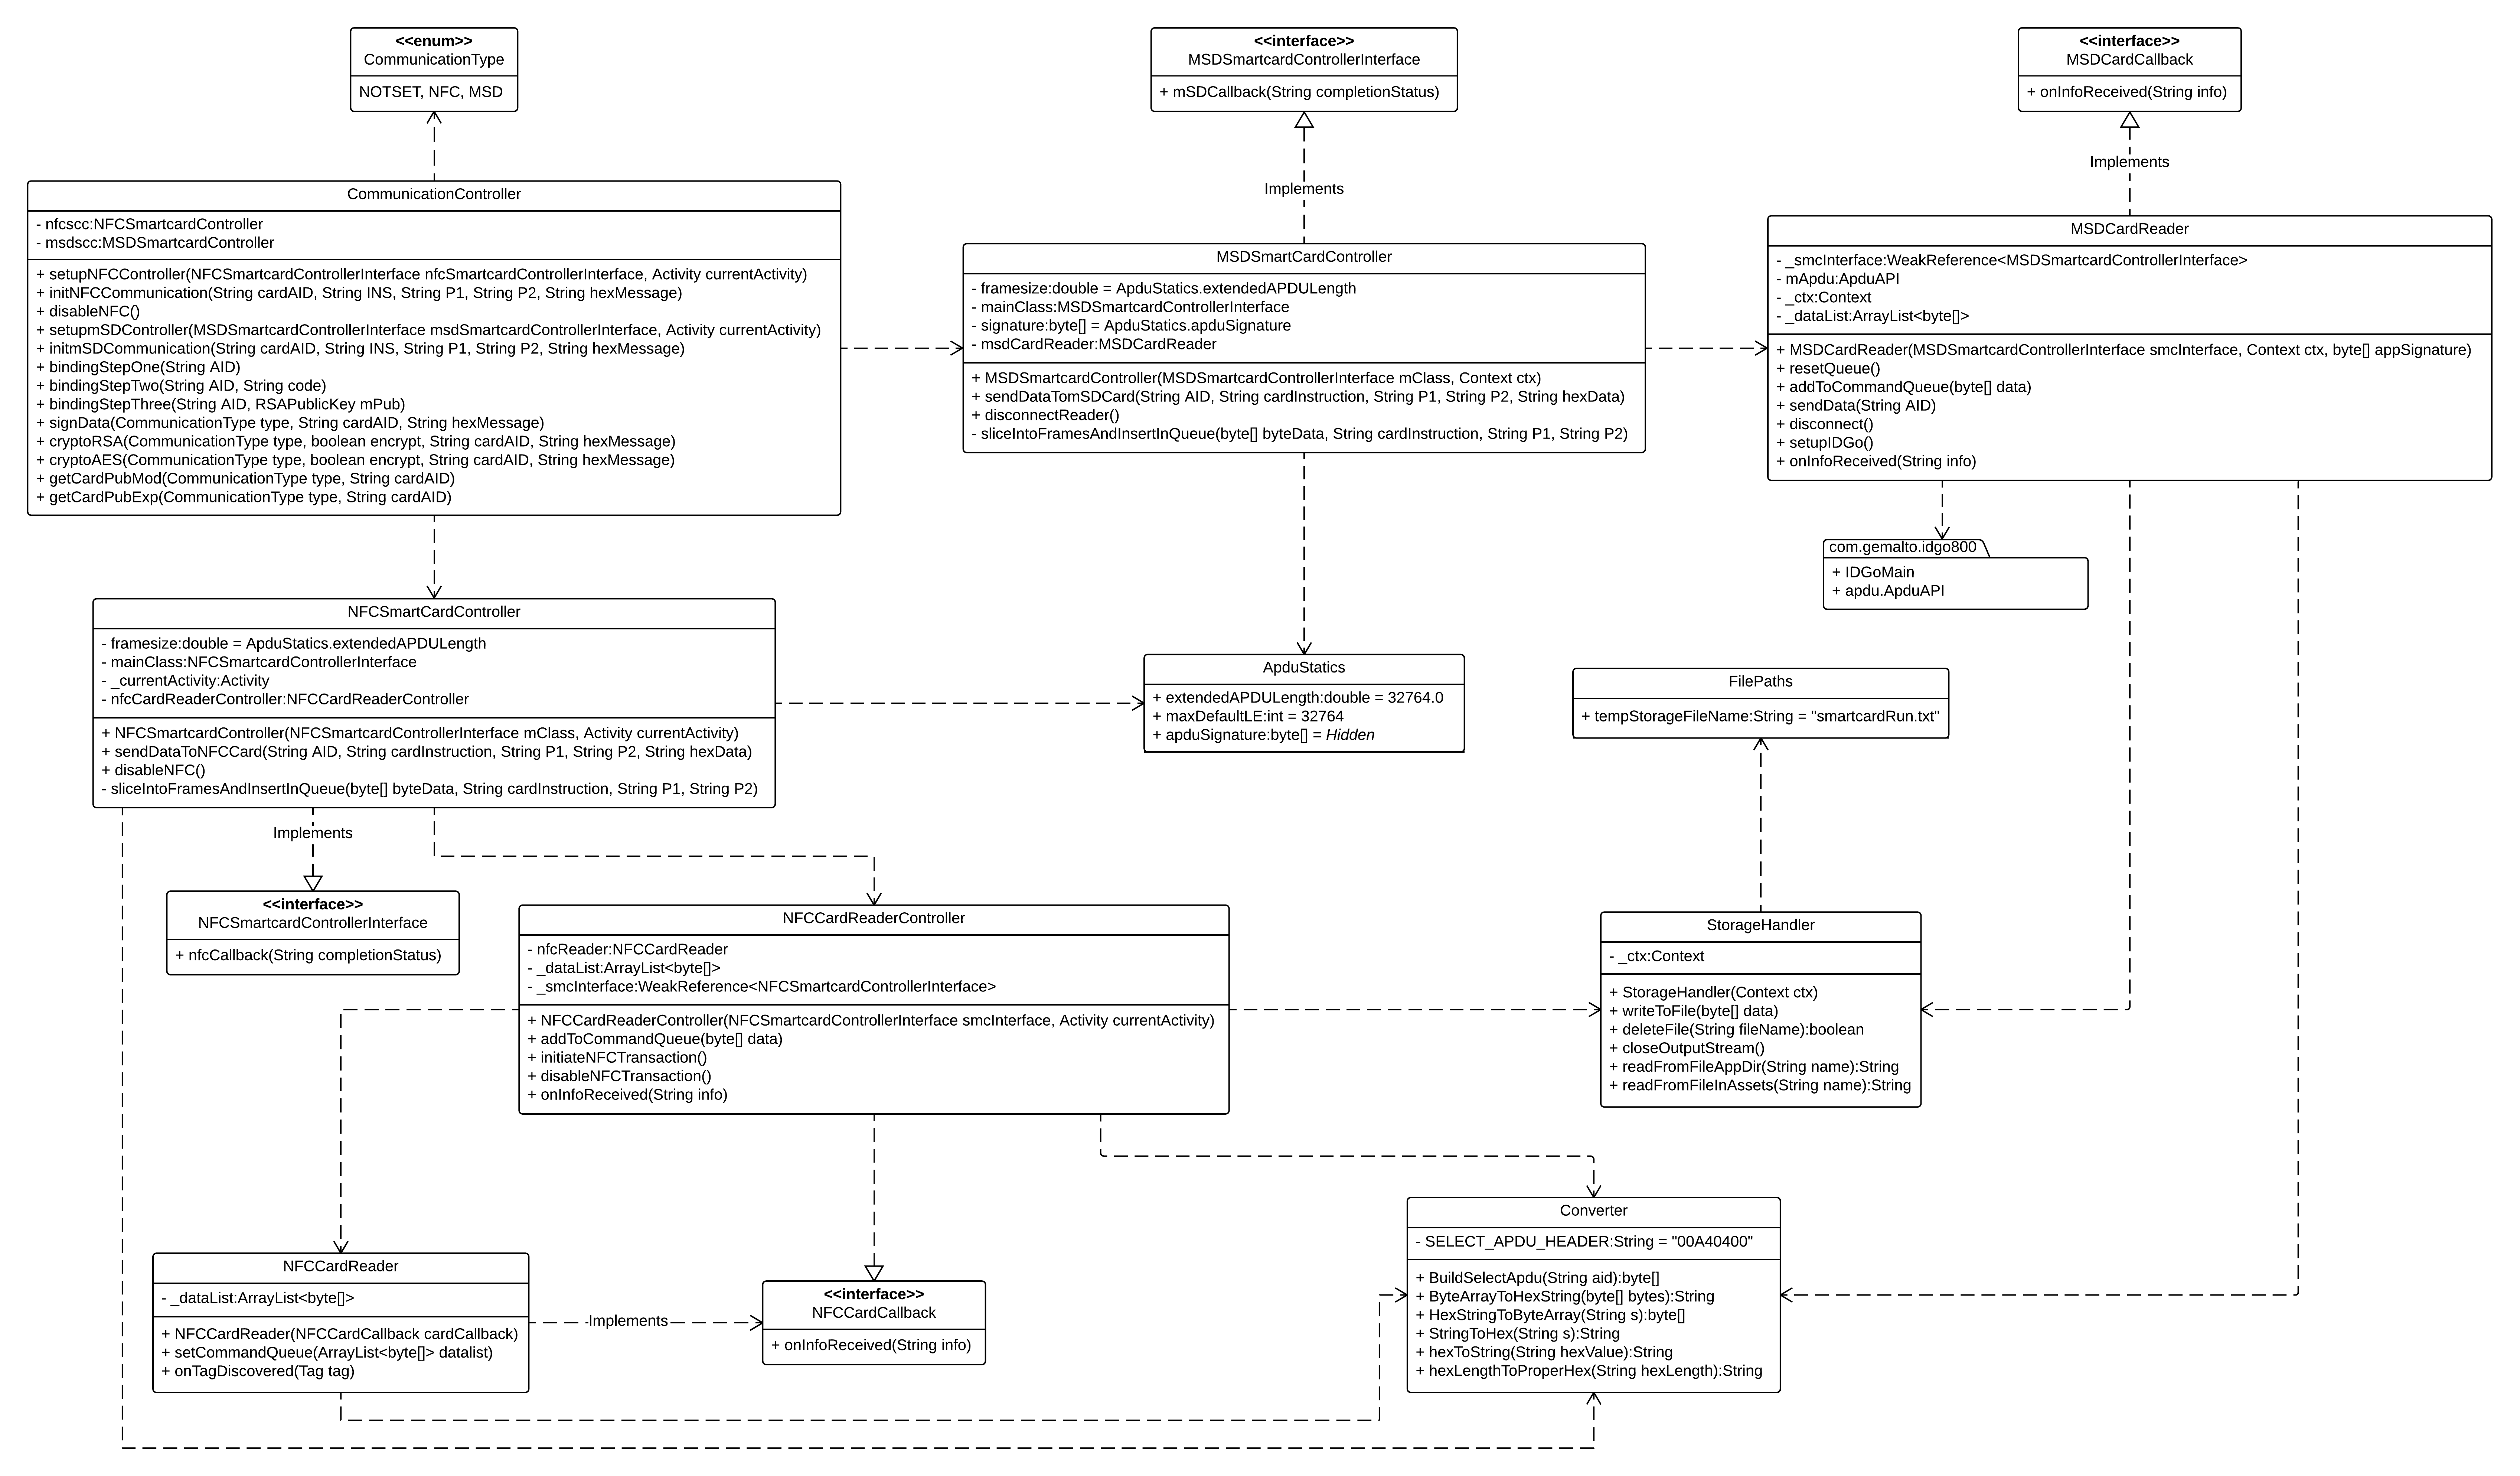
\includegraphics[width=0.95\textwidth]{images/Class_Diagram_Extended_Desc.png}
\end{figure}

% !TEX root = ../../Article.tex
\chapter{Framework installation}
\label{app:D}
\section{Smart card development environment}
Setup guide for developing smart card applications using Eclipse 3.2.
\begin{enumerate}
  \item Unzip ``Smart\_card.zip''
  \item Install Java Development Kit 6u45. Use ``jdk-6u45-windows-i586.exe'' for 32-bit Windows. Other operating system versions can be found at: \sloppy \url{http://www.oracle.com/technetwork/java/javase/downloads/java-archive-downloads-javase6-419409.html#jdk-6u45-oth-JPR}
  \item Copy the contents of ``java\_card\_kit-2\_2\_2-windows'' to a directory of your choice.
  \item Copy the contents of ``eclipse-SDK-3.2.2-win32'' to a directory of your choice.
  \item Copy the contents from ``eclipse-jcde-0.2\\plugins'' into the plugin folder for Eclipse from previous step.
  \item Start Eclipse using the batch script ``RUN\_ME.bat''.
  \item In the toolbar select ``Java Card \textrightarrow Preferences'' and make sure the Java Card Development Kit path points to where the kit was installed. Refer to figure \ref{fig:javacardkit}.
  \item In the toolbar select ``JCWDE \textrightarrow Preferences'' and make sure the Java Card Development Kit path points to where the kit was installed. Refer to figure \ref{fig:javacardkit}.

\end{enumerate}

\begin{figure}[h!]
  \caption{Configuring Java Card kit 2.2.2 for Eclipse.}
  \label{fig:javacardkit}
  \centering
    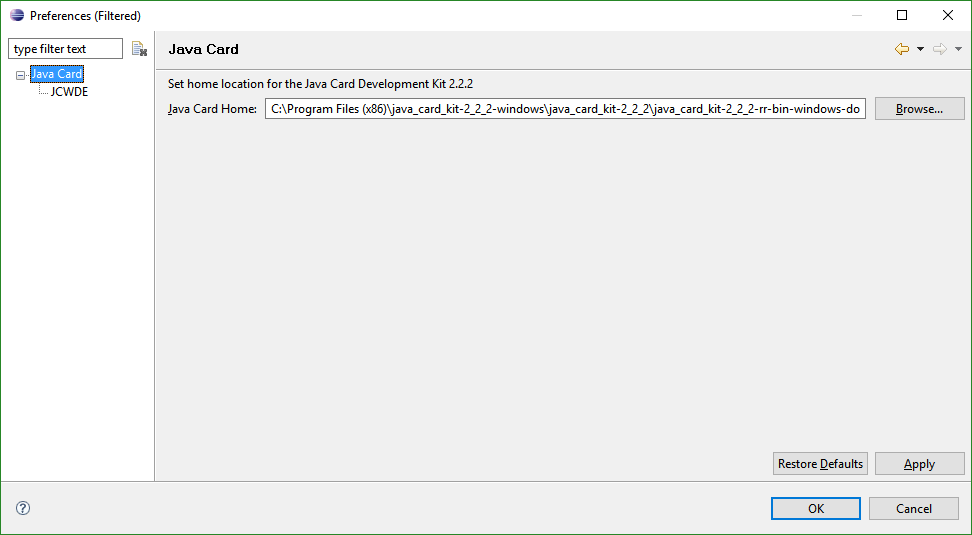
\includegraphics[width=0.95\textwidth]{images/eclipse_javacard.png}
\end{figure}

\section{Smart card deployment}
Setup guide for deploying smart card applications using GlobalPlatformPro (GP).
\begin{enumerate}
  \item Copy the contents of ``Smart\_card\_deployment'' to a directory of your choice.
  \item Configure ``runMe.bat'' and point to the correct .cap file.
  \item Run ``runMe.bat'' to delete and install your smart card application.
\end{enumerate}

\section{Smart card testing}
Setup guide for testing smart card applications using PyAPDUTool.
\begin{enumerate}
  \item Copy the contents of ``Smart\_card\_test\_tools'' to a directory of your choice.
  \item Run the tools.
\end{enumerate}

\section{Android development environment}
Setup guide for developing Android applications with our smart card library using Android Studio.
\begin{enumerate}
  \item Download the newest version of Android Studio from \sloppy \url{http://developer.android.com/sdk/index.html}
  \item Install Android SDK 6.0 using the Android SDK Manager.
  \item Add the libraries ``gPKIKeyStore'' and ``smartcardLibrary'' to your Android application. \sloppy \url{http://developer.android.com/sdk/installing/create-project.html#ReferencingLibraryModule}
  \item Fix any potential path issues.
\end{enumerate}




  \addcontentsline{toc}{section}{References}
  \printbibliography

\end{document}
